\documentclass[a4paper,10pt]{book}
\usepackage{lmodern}
\usepackage[centertags]{amsmath}
\usepackage{amscd}
\usepackage{amsthm}
\usepackage{amssymb}
\usepackage{enumerate}
\usepackage{multicol}
\usepackage[english,catalan,spanish]{babel}
\usepackage[all]{xy}
\usepackage{color}
\usepackage{tikz}
\usepackage{indentfirst}
\usepackage[utf8]{inputenc}
\usepackage[T1]{fontenc}
\linespread{1.1}
\setlength{\parskip}{10pt}
\usepackage[twoside,bindingoffset=1cm]{geometry}
\usepackage[x11names, dvipsnames, table]{xcolor}
\definecolor{ubblue}{HTML}{0059A2}
\usepackage[colorlinks=true, linkcolor=black, citecolor=ubblue, urlcolor=ubblue]{hyperref}
\usepackage{cleveref}
\usepackage[protrusion=true,expansion=true]{microtype}
\usepackage{cite}
\usepackage{booktabs}
\usepackage{IEEEtrantools}
\usepackage{subcaption}
\usepackage{enumitem}
\setlist[itemize]{itemsep=4pt, parsep=2pt, topsep=2pt, leftmargin=*}
\setlist[enumerate]{itemsep=4pt, parsep=2pt, topsep=2pt, leftmargin=*}
\usepackage{chronology}
\usepackage{longtable}
\usepackage{dirtree}
\usepackage{tabularx}
\usepackage{caption}
\captionsetup[table]{labelfont=bf}


%%%%%%%%%%%%%%%%%%%%%%%%%%%%%%%%%%%%%%%%%%%%%%%%%%%%%%%%%%%%%%%%%%%%%%%%%%%
%%%% local definitions for this paper
%%%%%%%%%%%%%%%%%%%%%%%%%%%%%%%%%%%%%%%%%%%%%%%%%%%%%%%%%%%%%%%%%%%%%%%%%%%






%%%%%%%%%%%%%%%%%%%%%% aix{\`o} pels headings %%%%%%%%%%%%%%%%%%%%%%%%
\usepackage{fancyhdr}
\pagestyle{fancy}
\renewcommand{\chaptermark}[1]{\markboth{#1}{}}
\renewcommand{\sectionmark}[1]{\markright{\thesection\ #1}}
\fancyhf{} \fancyhead[LE,RO]{\bfseries\thepage}
\fancyhead[LO]{\bfseries\rightmark} \fancyhead[RE]{\bfseries\leftmark}

\def\paginaenblanc{\newpage%
\thispagestyle{empty}%
\vspace*{2cm}%
\newpage%
\thispagestyle{empty}%
}


%%%%%%%%%%%%%%%%%%%%%%%%%%%%%%%%%%%%%%%%%%%%%%%%%%%%%%%%%%%%%%%%%%%%%%%%%
% aux commands
%%%%%%%%%%%%%%%%%%%%%%%%%%%%%%%%%%%%%%%%%%%%%%%%%%%%%%%%%%%%%%%%%%%%%%%%%
%==========================================================================
% macros to support private authors' notes
%==========================================================================
\newif\ifprivate
\privatetrue
\def\xbar{\vskip0.09in\hrule\vskip0.06in}
\def\private#1{\ifprivate \xbar {\em #1} \xbar
\else \fi}
\def\huh{\ifprivate ??? \marginpar{\Huge ???}
\else \fi}
\def\???{\ifprivate {\bf {???}} \marginpar{\begin{center}{\Huge {\bf ?}}\end{center}}
\else \fi}
%\def\???{\ifprivate {\bf {???}} \marginpar{{\Huge {\bf ?}}}
%\else \fi}
\marginparsep1mm
\def\nota#1{\ifprivate  $\clubsuit$ \marginpar{\parbox[t]{2.4cm}{\begin{center}\tiny #1\end{center}}}
\else \fi}
\def\comment#1{\ifprivate \marginpar{\parbox[t]{2.4cm}{\begin{center}\tiny #1\end{center}}}
\else \fi}
%\def\nota#1{\ifprivate  $\clubsuit$ \marginpar{\parbox[t]{1.8cm}{\tiny #1}}
%\else \fi}
\def\privateeject{\ifprivate\eject\fi}
%\def\???{{\bf {???}} \marginpar{{\Huge {\bf ?}}} }
%%%%%%%%%%%%%%%%%%%%%%%%%%%%%%%%%%%%%%%%%%%%%%%%%%%%%%%%%%%%%%%%%%%%%%%%%%

%%%%%%%%%%%%%% definicions cap{\'\i}tol ""%%%%%%%%
%%%%%%%%%%%%%%%%%%%%%%%%%%%%%%%%%%
\def\av{\underline{a}}

\def\Zr{\mathbb Z^r} \def\Nr{\mathbb N^r}
\def\xv{\underline{x}}
\def\yv{\underline{y}}
\def\zv{\underline{z}}

\newcommand{\Proj}{\operatorname{Proj}}
\newcommand{\Spec}{\operatorname{Spec}}


\def\HiRIM#1{H^i_{\mathcal M}(#1)}

\newcommand{\im}{\operatorname{Im}}
\renewcommand{\ker}{\operatorname{Ker}}
\newcommand{\grade}{\operatorname{grade}}
\newcommand{\Ext}{\operatorname{Ext}}
\newcommand{\Hom}{\operatorname{Hom}}
\newcommand{\m}{\mathfrak m}
\newcommand{\n}{\mathfrak n}
\newcommand{\M}{\mathfrak m}
%\newcommand{\cL}{{\mathcal L}}
\newcommand{\cP}{{\mathcal P}}
\newcommand{\cE}{{\mathcal E}}
\newcommand {\ZZ}{\mathbb{Z}}
\newcommand{\cS}{{\mathcal S}}
\newcommand {\PP}{\mathbb{P}}

\def\p{\mathfrak{p}}
\def\q{\mathfrak{q}}
\DeclareMathOperator{\de}{deg}

\DeclareMathOperator{\Hl}{H}
 \DeclareMathOperator{\h}{h}

%%%%%%%%%%%%%%%%%%%%%%%%%%%%%%%%%%%%%%%%%%%%%%%%%%%%%%%%%%%%%%%%%%%%%%%%%
%%%%%%%%%%%%%%%%%%%%%%%%%%%%%%%%%%%%%%%%%%%%%%%%%%%%%%%%%%%%%%%%%%%%%%%%%
%%%%%%%%%%%%%%%%%%%%%%%%%%%%%%%%%%%%%%%%%%%%%%%%%%%%%%%%%%%%%%%%%%%%%%%%%
%%%%%%%%%%%%%%%%%%%%%%%%%%%%%%%%%%%%%%%%%%%%%%%%%%%%%%%%%%%%%%%%%%%%%%%%%
%%%%%%%%%%%%%%%%%%%%%%%%%%%%%%%%%%%%%%%%%%%%%%%%%%%%%%%%%%%%%%%%%%%%%%%%%
%%%%%%%%%%%%%%%%%%%%%%%%%%%%%%%%%%%%%%%%%%%%%%%%%%%%%%%%%%%%%%%%%%%%%%%%%
%%%%%%%%%%%%%%%%%%%%%%%%%%%%%%%%%%%%%%%%%%%%%%%%%%%%%%%%%%%%%%%%%%%%%%%%%
%%%%%%%%%%%%%%%%%%%%%%%%%%%%%%%%%%%%%%%%%%%%%%%%%%%%%%%%%%%%%%%%%%%%%%%%
%%%%%%%%%%%%%%%%%%%%%%%%%%%%%%%%%%%%%%%%%%%%%%%%%%%%%%%%%%%%%%%%%%%%%%%%
\begin{document}
\pagestyle{empty}
\bstctlcite{IEEEexample:BSTcontrol}
\begin{titlepage}
	\begin{center}
		\begin{figure}[htb]
			\begin{center}
				
\includegraphics[width=6cm]{assets/ub_color.pdf}
			\end{center}
		\end{figure}
				
		\def\worktitle{Evaluación de Modelos Basados en Transformadores para la Clasificación de Subtipos Moleculares del Carcinoma Ductal Invasivo de Mama Mediante Mamografía}
				
		\textbf{\LARGE Treball final de grau} \\
		\vspace*{.5cm}
		\textbf{\LARGE GRAU D'ENGINYERIA INFORM\`{A}TICA } \\
		\vspace*{.5cm}
		\textbf{\LARGE Facultat de Matem\`atiques i Inform\`atica\\ Universitat de Barcelona} \\
		\vspace*{1.0cm}
		\rule{16cm}{0.1mm}\\
		\begin{Huge}
			\textbf{Evaluación de Modelos Basados en Transformers para la Clasificación de Subtipos Moleculares del Carcinoma Ductal Invasivo} \\
		\end{Huge}
		\rule{16cm}{0.1mm}\\
				
		\vspace{1cm}
				
		\begin{flushright}
						
						
			\vspace*{2.5cm}
						
			\hfill
						
			\renewcommand{\arraystretch}{1.5}
			\begin{tabular}{ll}
				\textbf{\small Autor:}       & \textbf{\small David Bland\'on T\'orrez }                             \\
				\textbf{\small Director:}    & \textbf{\small Dr. Oliver D\'iaz Montesdeoca }                        \\
				\textbf{\small Realitzat a:} & \textbf{\small  Departament de Matem\`{a}tiques i  Inform\`{a}tica  } \\
				\textbf{\small Barcelona,}   & \textbf{\small \today }                                               
			\end{tabular}
						
		\end{flushright}
				
	\end{center}
		
\end{titlepage}


%%%%%%%%%%%%%%%%%%%%%%%%%%%%%%%%%%%%%%%%%%%%%%%%%%%%%%%%%%%%%%%%%%%%%%%%%
\newpage
\selectlanguage{spanish}
\noindent \textbf{\large Resumen}

El cáncer de mama sigue siendo la neoplasia maligna más prevalente y una de las principales causas de mortalidad en mujeres a nivel mundial. La caracterización molecular temprana y precisa es crucial para el pronóstico y la selección de tratamientos. La subtipificación molecular, tradicionalmente basada en biopsias tisulares invasivas y análisis inmunohistoquímicos, permite terapias personalizadas, pero resulta costosa, consume tiempo y no siempre es viable. Las alternativas no invasivas que aprovechan imágenes médicas, particularmente la mamografía, han ganado interés investigativo para la clasificación molecular.

Este estudio evalúa el potencial de modelos de aprendizaje profundo basados en Transformers para clasificar subtipos moleculares de carcinoma ductal invasivo utilizando exclusivamente imágenes mamográficas del conjunto de datos público CMMD (The Chinese Mammography Database). Comparamos sistemáticamente tres arquitecturas Transformer de vanguardia: Vision Transformer (ViT), Swin Transformer (Swin) y Multi-Axis Vision Transformer (MaxViT), frente a una red neuronal convolucional (CNN) tradicional, ResNet-101. La metodología experimental aborda desafíos clave como el desbalance de clases mediante funciones de pérdida ponderadas, sobremuestreo, aumentación de datos y estrategias robustas de validación cruzada.

Los resultados indican que los modelos basados en Transformers superan consistentemente a la CNN de referencia. ViT logró el mayor AUC promedio (0.635 ± 0.016) y precisión balanceada (0.385 ± 0.042) en los conjuntos de prueba, frente a ResNet-101 (AUC: 0.563 ± 0.03; precisión balanceada: 0.322 ± 0.062). El análisis estadístico confirma diferencias significativas (p < 0.05), respaldando la hipótesis de que los mecanismos de autoatención en Transformers modelan mejor las relaciones espaciales globales en mamografías.

A pesar de estos avances, el rendimiento general sigue estando por debajo de los umbrales clínicamente aceptables, subrayando la dificultad inherente de la subtipificación molecular no invasiva basada únicamente en imágenes y la necesidad de investigar con conjuntos de datos más amplios o integración multimodal. No obstante, este trabajo demuestra el potencial de los enfoques basados en Transformers para caracterizar el cáncer de mama de manera accesible y no invasiva, estableciendo un referente sólido para futuros avances en imágenes médicas impulsadas por IA.

\newpage
\selectlanguage{english}
\noindent \textbf{\large Abstract}

Breast cancer remains the most prevalent malignancy and a leading cause of mortality in women worldwide. Early and accurate molecular characterization is critical for prognosis and treatment selection. Molecular subtyping, traditionally guided by invasive tissue biopsies and immunohistochemical analysis, enables personalized therapies but is costly, time-consuming, and not universally feasible. Non-invasive alternatives leveraging medical imaging, particularly mammography, have gained research interest for molecular classification.

This study evaluates the potential of Transformer-based DL models to classify molecular subtypes of invasive ductal carcinoma using mammographic images exclusively from the public CMMD (The Chinese Mammography Database)  dataset. A systematical analysis was conducted to compare three state-of-the-art Transformer architectures, Vision Transformer (ViT), Swin Transformer (Swin), and Multi-Axis Vision Transformer (MaxViT), against a traditional CNN model, ResNet-101. The experimental methodology addresses key challenges such as class imbalance through weighted loss functions, oversampling, data augmentation, and robust cross-validation strategies.

Results demonstrate that transformer-based models consistently outperform the CNN baseline. ViT achieved the highest average AUC (0.635 ± 0.016) and balanced accuracy (0.385 ± 0.042) on test sets, compared to ResNet-101 (AUC: 0.563 ± 0.03; balanced accuracy: 0.322 ± 0.062). Statistical analysis confirmed significant performance differences (p < 0.05), supporting the hypothesis that transformer self-attention mechanisms better model global spatial relationships in mammograms.

Despite these advances, overall performance remains below clinically acceptable thresholds, highlighting the inherent difficulty of non-invasive molecular subtyping based solely on imaging and the need for larger datasets or multimodal integration. Nevertheless, this work demonstrates the potential of transformer-based approaches for accessible, non-invasive breast cancer characterization, establishing a robust foundation for future AI-driven advancements in medical imaging.

\newpage
\selectlanguage{catalan}
\noindent \textbf{\large Resum}

El càncer de mama continua sent la neoplàsia maligna més prevalent i una de les principals causes de mortalitat en dones a nivell mundial. La caracterització molecular precoç i precisa és crucial per al pronòstic i la selecció de tractaments. La subtipificació molecular, tradicionalment basada en biòpsies tissulars invasives i anàlisi immunoistoquímics, permet teràpies personalitzades, però resulta costosa, consumeix temps i no sempre és viable. Les alternatives no invasives que aprofiten imatges mèdiques, particularment la mamografia, han guanyat interès investigador per a la classificació molecular.

Aquest estudi avalua el potencial de models d'aprenentatge profund (DL) basats en Transformers per classificar subtipus moleculars de carcinoma ductal invasiu utilitzant exclusivament imatges mamogràfiques del conjunt de dades públic CMMD. Comparem sistemàticament tres arquitectures Transformer d'avantguarda: Vision Transformer (ViT), Swin Transformer (Swin) i Multi-Axis Vision Transformer (MaxViT), front a una xarxa neuronal convolucional (CNN) tradicional, ResNet-101. La metodologia experimental aborda reptes clau com el desequilibri de classes mitjançant funcions de pèrdua ponderades, sobremostreig, augmentació de dades i estratègies robustes de validació creuada.

Els resultats indiquen que els models basats en Transformers superen consistentment la CNN de referència. ViT va assolir el major AUC mitjà (0,635 ± 0,016) i precisió balancejada (0,385 ± 0,042) en els conjunts de prova, front a ResNet-101 (AUC: 0,563 ± 0,03; precisió balancejada: 0,322 ± 0,062). L'anàlisi estadística confirma diferències significatives (p < 0,05), recolzant la hipòtesi que els mecanismes d'autoatenció en Transformers modelen millor les relacions espacials globals en mamografies.

Malgrat aquests avenços, el rendiment global segueix estant per sota dels llindars clínicament acceptables, subratllant la dificultat inherent de la subtipificació molecular no invasiva basada únicament en imatges i la necessitat d'investigar amb conjunts de dades més amplis o integració multimodal. No obstant això, aquest treball demostra el potencial dels enfocaments basats en Transformers per caracteritzar el càncer de mama de manera accessible i no invasiva, establint un referent sòlid per a futurs avenços en imatges mèdiques impulsades per IA.

\newpage
\selectlanguage{english}
\noindent \textbf{\large Agradecimientos}

En primer lugar, deseo expresar mi más profundo agradecimiento al Dr. Oliver Díaz Montesdeoca por su guía, paciencia y apoyo incondicional a lo largo de este proceso. Sus valiosos consejos y mentoría han sido fundamentales para la realización de este trabajo.

Dedico este logro a mi familia, a quienes están con nosotros y a quienes ya no están, especialmente a mis padres y hermanos. Gracias por vuestro amor incondicional, por creer en mí y por ser siempre mi mayor inspiración; sin vosotros no sería la persona que soy hoy.

También extiendo mi gratitud a mi segunda familia, Martha y Adriana, por su constante ánimo y por cuidarme en cada etapa de este camino.

Igualmente, agradezco a mis amigos Jose, Sergio, Teo y Jordi, por hacer de la universidad un lugar más agradable y por su incomparable compañía.

Y, sobre todo, gracias a Mabel, por ser la energía y la luz de mi vida. \textit{Todo esto es por ti}.

\selectlanguage{spanish}
\pagenumbering{roman} \setcounter{page}{0}
\let\cleardoublepage\clearpage
\tableofcontents
\newpage \thispagestyle{empty}
%%%%%%%%%%%%%%%%%%%%%%%%%%%%%%%%%%%%%%%%%%%%%%%%%%%%%%%%%%%%%%%%%%%%%%%%%

\listoffigures
\listoftables


%%%%%%%%%%%%%%%%%%%%% aix{\`o} pels headings %%%%%%%%%%%%%%%%%%%%%%%%
\pagestyle{fancy}
\markboth{Introduction}{Introducción}
\newpage \thispagestyle{empty}


%%%%%%%%%%%%%%%%%%%%%%%%%%%%%%%%%%%%%%%%%%%%%%%%%%%%%%%%%%%%%%%%%%%%%%%%%
\mainmatter
\chapter{Introducción}
\section{Contexto del problema}

El cáncer de mama es una de las principales causas de mortalidad entre las mujeres y el tipo de cáncer más común en esta población. Se estima que, en promedio, una de cada veinte mujeres en todo el mundo será diagnosticada con cáncer de mama a lo largo de su vida \cite{kim_global_2025}. Proyecciones recientes sugieren que, si la tendencia actual continúa, para el año 2050 habrá aproximadamente 3,2 millones de nuevos casos y 1,1 millones de muertes por esta enfermedad, con un impacto particularmente significativo en países con bajos índices de desarrollo humano (IDH) \cite{kim_global_2025}.

En este contexto, el diagnóstico precoz y las herramientas de imagen diagnóstica desempeñan un papel fundamental en la mejora del pronóstico y la supervivencia de las pacientes \cite{wang_early_2017}. Sin embargo, el cáncer de mama es una enfermedad heterogénea\footnote{Diversidad celular presente dentro de un tumor (heterogeneidad intratumoral) o entre diferentes tumores en un mismo individuo (heterogeneidad intertumoral).} que puede clasificarse en varios subtipos según características clínicas y, especialmente, moleculares. Las Directrices del Consenso Internacional de St. Gallen de 2013 \cite{goldhirsch_personalizing_2013} definieron cuatro subtipos principales basados en los receptores hormonales (estrógeno y progesterona) y el marcador de proliferación Ki67: Luminal A, Luminal B, HER2 positivo (HER2-enriquecido) y Triple Negativo (véase la Figura \ref{fig:subtypes}). Esta clasificación tiene implicaciones clínicas directas, ya que el pronóstico, la respuesta terapéutica y las opciones de tratamiento están en gran medida determinados por el subtipo molecular del tumor.

Actualmente, la caracterización molecular del tumor se realiza principalmente mediante biopsia tisular, un procedimiento invasivo y costoso que puede requerir repetición, lo que potencialmente retrasa el inicio del tratamiento e incrementa la carga clínica, física y emocional sobre las pacientes. Por ello, existe una necesidad creciente de desarrollar métodos no invasivos, accesibles y eficientes para la clasificación fiable de los subtipos moleculares. En este sentido, la mamografía por rayos X destaca como la modalidad de imagen de referencia, ya que es una técnica no invasiva, de bajo coste y ampliamente utilizada para el cribado y diagnóstico del cáncer de mama, debido a su eficacia demostrada en la práctica clínica.

\begin{figure}
\center
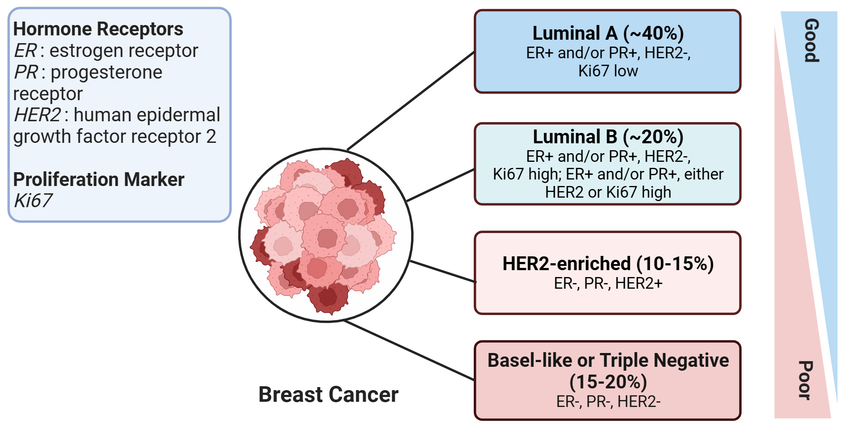
\includegraphics[width=0.8\linewidth]{reports/assets/subtypes.png} 
\caption[Clasificación de subtipos moleculares del cáncer de mama.]{Clasificación de subtipos moleculares del cáncer de mama, mostrando proporciones aproximadas (\%) entre todos los casos. Los subtipos están ordenados por severidad del pronóstico, con mejores resultados en la parte superior y pronósticos progresivamente peores hacia la base \cite{harnessing_2024}.} \label{fig:subtypes} 
\end{figure}

En los últimos años, los avances en inteligencia artificial (IA), junto con la creciente disponibilidad de datos y recursos computacionales más potentes, han impulsado el desarrollo de modelos de aprendizaje profundo (deep learning, DL) para clasificación, detección y predicción de pronóstico en cáncer de mama, así como aplicaciones en otras enfermedades. Varios estudios han demostrado que estos sistemas pueden igualar o incluso superar el rendimiento de expertos humanos o sistemas CAD\footnote{Diagnóstico Asistido por Computadora (Computer-Aided Diagnosis)} en estas tareas \cite{mckinney_international_2020,pattanaik_breast_2022,meenalochini_deep_2024,hussain_performance_2025}, destacando el potencial de esta tecnología para mejorar la práctica clínica y los resultados en pacientes.

Investigaciones recientes han explorado la clasificación de subtipos moleculares del cáncer de mama a partir de imágenes mamográficas. Por ejemplo, Mota et al. (2024) \cite{mota_breast_2024} abordaron este reto, logrando un área bajo la curva (AUC)\footnote{Métrica utilizada en aprendizaje automático para evaluar el rendimiento de modelos de clasificación.} multiclase del 60,62\% mediante una arquitectura ResNet-101. De manera similar, Rabah et al. (2025) \cite{ben_rabah_multimodal_2025} obtuvieron un AUC del 61,3\% con un modelo Xception en configuraciones unimodales\footnote{Uso de un único tipo de dato como entrada (imágenes, texto, vídeo, etc.).} y desarrollaron un enfoque multimodal que integra metadatos clínicos, alcanzando un 88,87\% de AUC. Si bien los enfoques unimodales muestran un rendimiento modesto que permanece por debajo de umbrales clínicamente aceptables (~80\% AUC), estos estudios resaltan el potencial diagnóstico de las imágenes mamográficas y subrayan la importancia de continuar investigando para mejorar la precisión y utilidad clínica de estos model

Este estudio propone un enfoque unimodal basado exclusivamente en inferencias a partir de mamografías de la base de datos pública CMMD (The Chinese Mammography Database) \cite{cai_online_2023}, comparando el rendimiento de arquitecturas Transformer de última generación —incluyendo Vision Transformer (ViT), Swin Transformer (Swin) y Multi-Axis Vision Transformer (MaxViT)— frente a una línea base tradicional con ResNet-101. Aunque los modelos multimodales suelen lograr resultados superiores al integrar datos clínicos complementarios, un enfoque unimodal centrado únicamente en imágenes mamográficas ofrece ventajas prácticas significativas, especialmente en entornos con recursos limitados o cuando no hay estandarización de datos clínicos. Estudios recientes demuestran que los modelos basados en Transformers superan a las redes neuronales convolucionales (CNN) en precisión y robustez para tareas de clasificación de imágenes médicas, gracias a sus mecanismos de autoatención que capturan relaciones espaciales globales en las imágenes \cite{mauricio_comparing_2023}. Basándonos en estas ventajas arquitectónicas, planteamos la hipótesis de que las arquitecturas Transformer lograrán un rendimiento superior en la clasificación de subtipos moleculares, incluso bajo un enfoque unimodal.

En última instancia, este trabajo busca contribuir al desarrollo de herramientas diagnósticas no invasivas mediante la evaluación sistemática de modelos basados en transformers, avanzando hacia una caracterización molecular automatizada, accesible y eficiente del cáncer de mama. Este enfoque resulta particularmente valioso en escenarios clínicos donde la biopsia tisular no es inmediatamente viable, pudiendo mejorar la equidad diagnóstica y reducir el tiempo de inicio del tratamiento.


\section{Planificación}

\subsection{Objetivos}

El \textbf{objetivo principal} de este estudio es comparar sistemáticamente arquitecturas basadas en Transformers frente a una línea base CNN para clasificación de subtipos moleculares mediante mamografías, estableciendo benchmarks de rendimiento para la caracterización no invasiva del cáncer de mama.

Para alcanzar este objetivo principal, se proponen los siguientes \textbf{objetivos secundarios}:

\begin{enumerate}
\item \textbf{Realizar una revisión bibliográfica exhaustiva} de enfoques de IA para clasificación de subtipos moleculares en cáncer de mama, analizando investigaciones actuales y métricas de rendimiento.
\item \textbf{Identificar y abordar desafíos del dataset} mediante estrategias de preprocesado apropiadas, incluyendo mitigación del desbalance de clases mediante funciones de pérdida ponderadas, técnicas de muestreo balanceado y métodos de aumento de datos.
\item \textbf{Desarrollar e implementar} un marco robusto de validación cruzada estratificada de k particiones para entrenar y evaluar arquitecturas Vision Transformer (ViT, Swin y MaxViT) en imágenes mamográficas.
\item \textbf{Establecer un análisis comparativo de rendimiento} frente a la línea base ResNet-101 y resultados de referencia de la literatura, utilizando métricas estandarizadas (Exactitud, AUC, F1-Score, Precisión, Sensibilidad, Cohen-Kappa).
\item \textbf{Realizar validación estadística} de las diferencias en rendimiento mediante pruebas estadísticas para garantizar significancia y confiabilidad de los resultados.
\item \textbf{Efectuar un análisis comparativo} con literatura reciente para identificar avances e implicaciones prácticas de los hallazgos.
\item \textbf{Aplicar análisis de interpretabilidad} mediante técnicas Grad-CAM y visualización de atención para identificar características mamográficas más relevantes en la discriminación de subtipos moleculares.
\item \textbf{Sintetizar hallazgos y proporcionar recomendaciones} para futuras líneas de investigación y consideraciones de implementación clínica.
\end{enumerate}

\subsection{Tareas a Desarrollar}

Para abordar los objetivos previamente mencionados del proyecto, se han identificado varias tareas, como se describe a continuación.

\textbf{Estado del Arte}

\begin{enumerate}
\item \textbf{Contexto médico}: Revisar la literatura científica actual sobre el cáncer de mama para contextualizar su relevancia clínica y epidemiológica.
\item \textbf{Intuición del problema}: Analizar la importancia de la caracterización molecular en el cáncer de mama, destacando sus ventajas, limitaciones y desafíos actuales.
\item \textbf{Trabajos previos}: Examinar los avances recientes en inteligencia artificial y aprendizaje profundo para la caracterización y diagnóstico del cáncer de mama, comparando enfoques y resultados reportados en la literatura.
\end{enumerate}

\textbf{Implementación}

\begin{enumerate}
\item \textbf{Recolección de datos}: Adquirir imágenes y familiarizarse con la estructura, organización y metadatos proporcionados del conjunto de datos.
\item \textbf{Análisis y preprocesamiento de datos}: Analizar la distribución de clases, la consistencia de los datos y realizar el preprocesamiento de imágenes.
\item \textbf{Codificación del proyecto}: Desarrollar el código para realizar experimentos, entrenar y evaluar los diferentes modelos.
\item \textbf{Análisis de resultados}: Evaluar e interpretar los resultados para extraer conclusiones y proponer trabajos futuros.
\end{enumerate}

\textbf{Preparación del Informe}

\begin{enumerate}
\item \textbf{Redacción del informe}: Documentar todos los procedimientos, incluyendo metodología, materiales, resultados y conclusiones.
\item \textbf{Revisiones}: Incorporar el feedback del asesor y refinar hasta alcanzar una calidad aceptable.
\item \textbf{Entrega y presentación}: Entregar la tesis y preparar un resumen de los hallazgos clave para la presentación ante el comité.
\end{enumerate}

\subsection{Planificación}

La planificación del proyecto se representa en el diagrama de Gantt que se muestra a continuación (Figura \ref{fig:roadmap}), donde se detallan las tareas previamente definidas a lo largo de los 4 meses del proyecto (Semestre de Primavera).

\begin{figure}[h!]
\centering
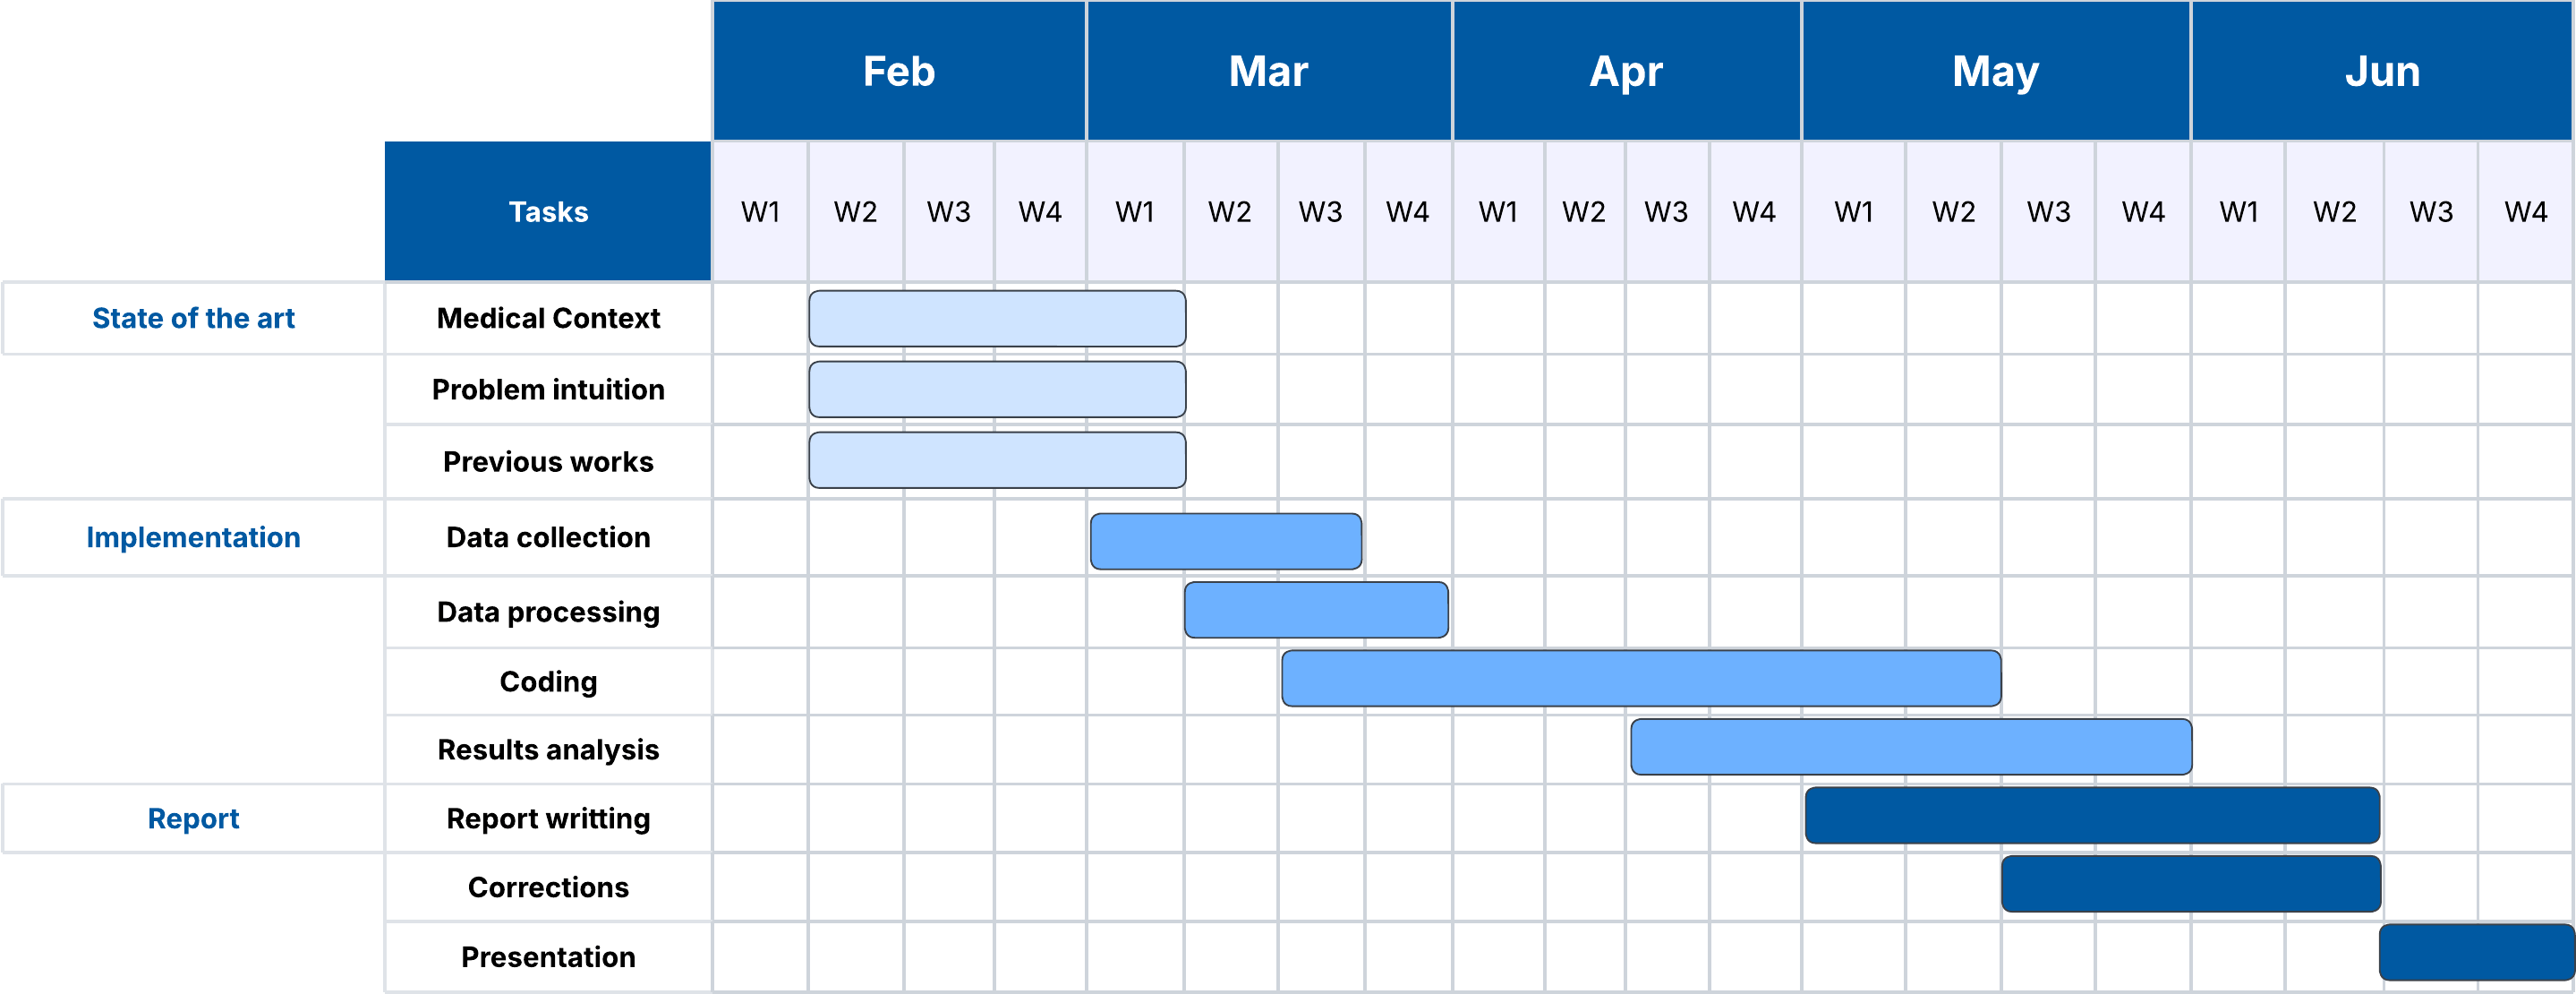
\includegraphics[width=1\linewidth]{reports//assets/RoadmapV3.png}
\caption[Diagrama de Gantt de planificación]{Diagrama de Gantt.}
\label{fig:roadmap}
\end{figure}



%%%%%%%%%%%%%%%%%%%%%%%%%%%%%%%%%%%%%%%%%%%%%%%%%%%%%%%%%%%%%%%%%%%%%%%%%

\chapter{Antecedentes}

\section{Cáncer de mama}

El cáncer de mama es una neoplasia maligna\footnote{Crecimiento anormal y descontrolado de células que da lugar a una masa o tumor, llamado benigno si crece lentamente y permanece localizado, o maligno si es invasivo y de crecimiento rápido.} que se origina en el tejido glandular de la mama, principalmente en los conductos y lobulillos, donde ciertas células sufren mutaciones genéticas que alteran el control de su crecimiento.

Estas alteraciones permiten que las células se multipliquen sin control, formando masas tumorales que pueden infiltrar los tejidos adyacentes e incluso diseminarse a órganos distantes a través del sistema linfático y el torrente sanguíneo. En ausencia de un diagnóstico temprano y un tratamiento oportuno, esta diseminación, también conocida como metástasis, puede comprometer gravemente la supervivencia del paciente. La figura \ref{fig:breast-cancer-anatomy} ilustra la estructura anatómica de la mama, mostrando cómo se desarrollan los tumores dentro del tejido mamario normal.

\begin{figure}[h]
	\centering
	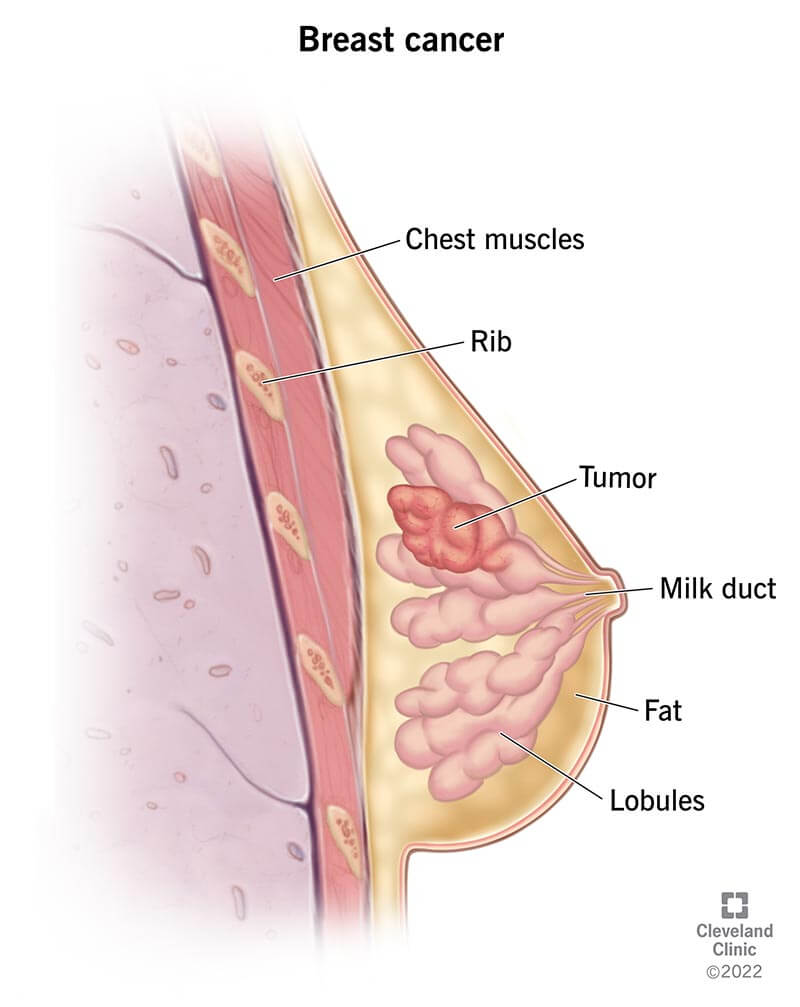
\includegraphics[width=0.3\linewidth]{reports//assets/bc.jpg}
	\caption[Anatomía del cáncer de mama]{Anatomía del cáncer de mama \cite{cleveland_clinic_breast_2023}.}
	\label{fig:breast-cancer-anatomy}
\end{figure}

\subsection{Epidemiología}

A nivel mundial, es la neoplasia más frecuente entre las mujeres y la principal causa de mortalidad relacionada con el cáncer en esta población. En 2022, se estimaron aproximadamente 2,3 millones de nuevos casos, con 670.000 muertes por esta enfermedad, según la Organización Mundial de la Salud (OMS) \cite{who_breast_2024}. En España, el cáncer de mama representa casi el 30\% de todos los casos de cáncer, y las proyecciones de la Sociedad Española de Oncología Médica (SEOM) estiman alrededor de 37.400 nuevos casos en 2025 \cite{seom_cancer_nodate}.

\subsection{Clasificación clínica}

La mayoría de los cánceres de mama son carcinomas, que son tumores malignos que se originan en los conductos o lobulillos de la mama. Estos carcinomas constituyen más del 95\% de todos los casos de cáncer de mama \cite{makki_diversity_2015, noauthor_types_nodate}. Desde una perspectiva clínica, estos tumores pueden clasificarse según varios criterios, entre los que destacan los siguientes:

\textbf{Según su grado de invasión}
\begin{itemize}
\item \textbf{Carcinoma in situ}: Tumor en el que las células anormales están confinadas dentro de los conductos mamarios y no han atravesado la barrera natural que las separa del resto del tejido mamario. Aunque no es invasivo, se considera una lesión precursora y de alto riesgo.
\item \textbf{Carcinoma invasivo}: Tumor que ha atravesado los conductos o lobulillos de la mama e invadido el tejido mamario circundante. Puede diseminarse a los ganglios linfáticos o a sitios distantes.
\end{itemize}

\textbf{Según el origen histológico}
\begin{itemize}
\item \textbf{Carcinoma ductal}: Se origina en los conductos galactóforos\footnote{Conductos que transportan la leche desde las glándulas mamarias hasta el pezón.} y es el subtipo más común.
\item \textbf{Carcinoma lobulillar}: Se origina en los lobulillos mamarios y tiende a mostrar un patrón de diseminación más difuso.
\end{itemize}

Las figuras \ref{fig:histological_types_one} y \ref{fig:histological_types_two} muestran las diferencias entre el carcinoma ductal y el lobulillar, tanto in situ como invasivos.

\begin{figure}[h!]
	\centering
	\begin{subfigure}[c]{0.48\textwidth}
		\centering
		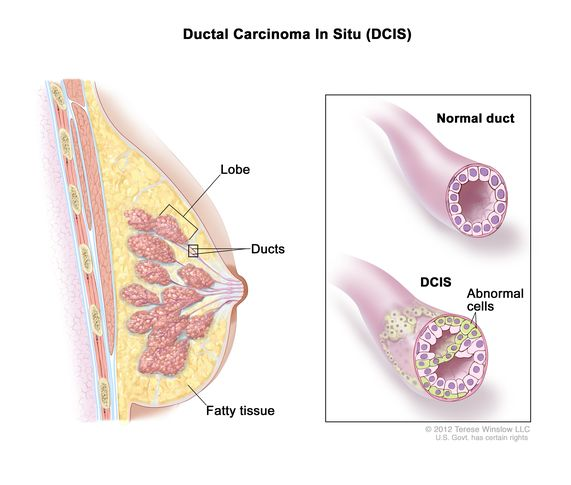
\includegraphics[width=\textwidth]{reports/assets/dcis.jpg}
		\caption{Carcinoma ductal in situ}
		\label{fig:dcis}
	\end{subfigure}
	\begin{subfigure}[c]{0.48\textwidth}
		\centering
		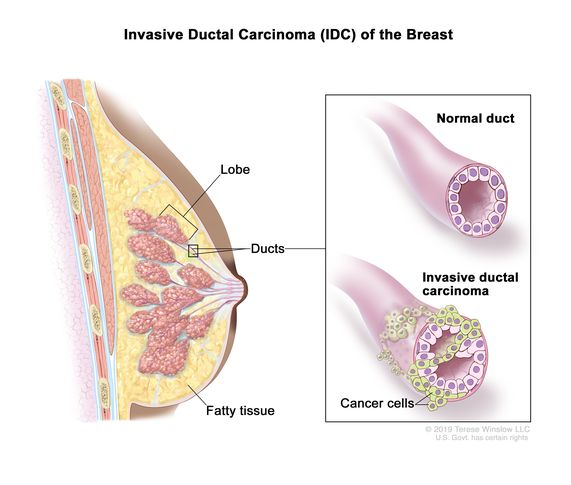
\includegraphics[width=\textwidth]{reports/assets/idc.jpg}
		\caption{Carcinoma ductal invasivo}
		\label{fig:idc}
	\end{subfigure}
	\caption[Comparación DCIS vs. IDC]{Comparación anatómica entre carcinoma ductal in situ (DCIS) y carcinoma ductal invasivo (IDC). (a) El DCIS muestra células anormales confinadas dentro de la estructura del conducto galactóforo, mientras que (b) el IDC demuestra células cancerosas que han atravesado la pared del conducto e invadido el tejido mamario circundante \cite{noauthor_nci_2011}.}
	\label{fig:histological_types_one}
\end{figure}

\begin{figure}[h!]
	\centering
	\begin{subfigure}[c]{0.48\textwidth}
		\centering
		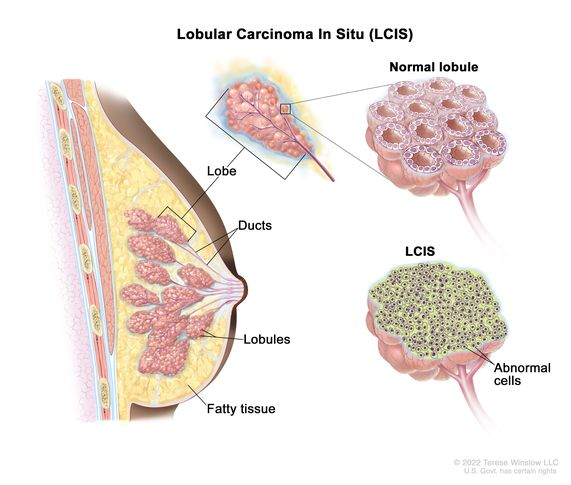
\includegraphics[width=\textwidth]{reports/assets/lcis.jpg}
		\caption{Carcinoma lobulillar in situ}
		\label{fig:lcis}
	\end{subfigure}
	\begin{subfigure}[c]{0.48\textwidth}
		\centering
		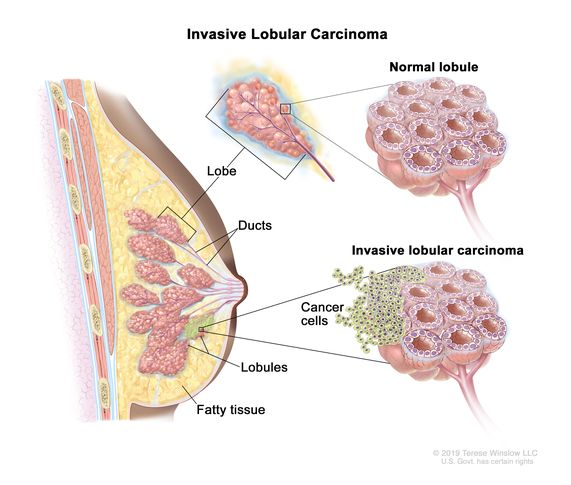
\includegraphics[width=\textwidth]{reports/assets/ilc.jpg}
		\caption{Carcinoma lobulillar invasivo}
		\label{fig:ilc}
	\end{subfigure}
	\caption[Comparación LCIS vs. ILC]{Progresión desde carcinoma lobulillar in situ (LCIS) hasta carcinoma lobulillar invasivo (ILC). (a) El LCIS representa el crecimiento anormal de células restringido a los lobulillos productores de leche, mientras que (b) el ILC muestra células malignas que se diseminan desde los lobulillos hacia el tejido mamario adyacente \cite{noauthor_nci_2011}.}
	\label{fig:histological_types_two}
\end{figure}

\textbf{Según los sistemas de estadificación}

Los sistemas clínicos de estadificación son una forma de determinar cuán extendido está el cáncer y hasta dónde se ha diseminado en el organismo, utilizando pruebas y evaluaciones realizadas antes de la cirugía u otro tratamiento. Esto proporciona marcos estandarizados para el pronóstico y la planificación terapéutica.

\begin{itemize}
	\item \textbf{Sistema de estadificación BI-RADS}: El Breast Imaging-Reporting and Data System (BI-RADS)\cite{magny_breast_2025} estandariza la interpretación mamográfica y asigna categorías de sospecha que guían el manejo médico (ver Tabla \ref{tab:birads_table}).
    \item  \textbf{Sistema de estadificación TNM}: Es el sistema de estadificación más utilizado \cite{noauthor_stages_nodate}. Evalúa tres factores anatómicos clave:
    \begin{itemize}
        \item \textbf{Tumor (T)}: Tamaño y extensión local del tumor primario, que va desde TX (el tumor no puede ser evaluado) hasta T4 (invasión local extensa).
        \item \textbf{Nódulo (N)}: Afectación de ganglios linfáticos regionales, desde NX (los ganglios linfáticos cercanos no pueden ser evaluados) hasta N3 (diseminación ganglionar extensa).
        \item \textbf{Metástasis (M)}: Presencia o ausencia de metástasis a distancia (M0 o M1).
  \end{itemize}
  El sistema TNM actual, actualizado en 2018, incorpora nuevos parámetros como el receptor de estrógenos (RE), el receptor de progesterona (RP) y otras variables clínicas para proporcionar una estratificación pronóstica más precisa \cite{hortobagyi_new_2018}. 
  
\end{itemize}

\begin{table}[h!]
	\caption[Breast Imaging-Reporting and Data System (BI-RADS)]{Clasificación del Breast Imaging-Reporting and Data System (BI-RADS) \cite{noauthor_bi-rads_2025}.}
	\centering
	\begin{tabular}{lccccc}
		\toprule
		\textbf{Categoría} & \textbf{Definición} & \textbf{Probabilidad de cáncer}\\
		\midrule
		BI-RADS 0        & Incompleto                         & N/A \\
		BI-RADS 1        & Negativo                           & Prácticamente 0\% \\
        BI-RADS 2        & Benigno                             & Prácticamente 0\%  \\
        BI-RADS 3        & Probablemente benigno               & > 0\% pero $\leq 2\%$ \\
        BI-RADS 4        & Sospechoso                          & > 2\% pero < 95\% \\
        BI-RADS 5        & Altamente sugestivo de malignidad   & $\geq 95\%$ \\
        BI-RADS 6        & Malignidad confirmada por biopsia   & N/A \\
		\bottomrule
	\end{tabular}
	\label{tab:birads_table}
\end{table}

Además de estas clasificaciones, en los últimos años ha cobrado especial relevancia la subtipificación molecular del cáncer de mama, basada en la expresión de biomarcadores y perfiles genómicos, cuestión que se abordará en la siguiente sección.


\subsection{Subtipos moleculares}

Aunque la clasificación clínica e histológica del cáncer de mama proporciona información importante para el diagnóstico, no siempre permite predecir con precisión el comportamiento biológico del tumor ni su respuesta a tratamientos específicos.

Las investigaciones de Perou et al. (2000) \cite{perou_molecular_2000} y Sørli et al. (2003) \cite{sorlie_repeated_2003} sentaron las bases para la caracterización molecular del cáncer de mama. Mediante el análisis de perfiles de expresión génica\footnote{Estudio que identifica qué genes están activos y en qué medida en una célula o tejido, analizando los niveles de ARN producidos por miles de genes simultáneamente.}, Perou et al. demostraron que el cáncer de mama es una enfermedad heterogénea y propusieron una clasificación molecular en subtipos basada en los patrones de expresión genética de los tumores analizados. Inicialmente se definieron cuatro subtipos: \textbf{Luminal A}, \textbf{Luminal B}, \textbf{HER2} y \textbf{Basal-like (Triple negativo)}.

Sørli et al. reforzaron estos hallazgos. Replicaron la investigación en diferentes cohortes de pacientes, demostrando que los resultados no eran artefactos de un solo estudio. También mostraron que los subtipos moleculares se asocian a diferencias clínicamente significativas, como el pronóstico y el riesgo de metástasis a distancia, otorgando a esta caracterización un mayor valor predictivo que la clasificación histológica tradicional.

\begin{figure}
	\centering
	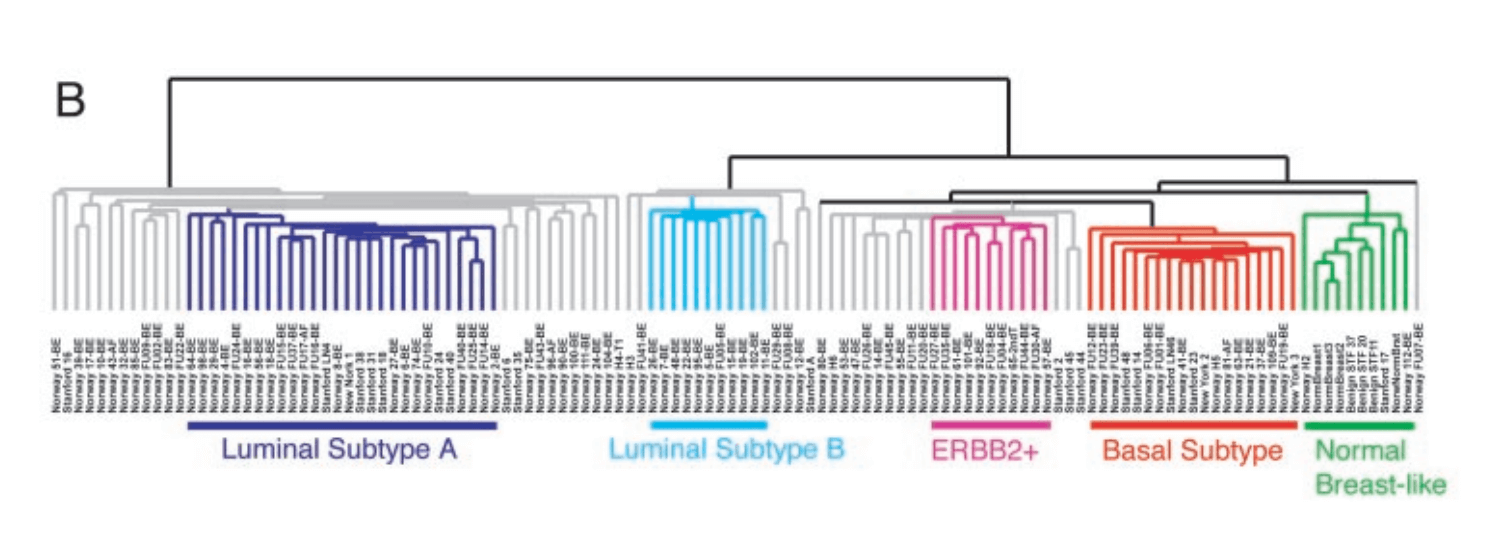
\includegraphics[width=0.8\linewidth]{reports//assets/dendogram.png}
	\caption[Dendrograma de subtipos moleculares según Sørli et al.]{Dendrograma del estudio de Sørli et al. que muestra la agrupación de subtipos según patrones genéticos \cite{sorlie_repeated_2003}.}
	\label{fig:sorlie-dandrogram}
\end{figure}


Tras estos estudios, los esfuerzos se centraron en trasladar los hallazgos a la práctica clínica. Dado que la técnica utilizada para la clasificación en ese momento (microarrays de ADN) era costosa, compleja y no accesible para la mayoría de los hospitales, se buscó una alternativa. Fue en las reuniones de consenso internacional de St. Gallen donde se propusieron criterios de clasificación basados en marcadores inmunohistoquímicos (IHQ)\footnote{Proteínas o antígenos específicos presentes en células o tejidos que pueden detectarse mediante anticuerpos en una técnica de laboratorio llamada inmunohistoquímica.}, formalizando los subtipos mediante la combinación de los siguientes receptores hormonales \cite{lips_breast_2013}:

\begin{itemize}
	\item \textbf{Receptores de estrógenos (RE) y progesterona (RP)}: Definen la dependencia hormonal del tumor, lo que puede afectar su crecimiento. Los tumores con estos receptores responden bien a la terapia hormonal.
	\item \textbf{HER2 (Receptor 2 del factor de crecimiento epidérmico humano)}: Proteína que estimula el crecimiento celular. Su sobreexpresión suele indicar un subtipo más agresivo.
	\item \textbf{Ki-67}: Índice de proliferación celular. Un Ki-67 elevado sugiere un tumor más agresivo y de rápida proliferación.
\end{itemize}

La Tabla \ref{tab:molecular_subtypes_comb} muestra estos criterios de clasificación.

\begin{table}[h!]
	\centering
        \caption[Criterios de clasificación de subtipos moleculares de cáncer de mama]{Criterios de clasificación de los subtipos moleculares según el consenso de St. Gallen 2013 \cite{goldhirsch_personalizing_2013}.}
	\begin{tabular}{lccccc}
		\toprule
		\textbf{Subtipo} & \textbf{HER2} & \textbf{RE} & \textbf{RP} & \textbf{Ki-67} \\
		\midrule
		Luminal A        & Negativo      & Positivo    & Positivo    & < 14\%         \\
		Luminal B/HER2-  & Negativo      & Positivo    & -           & $\geq$ 14\%    \\
		Luminal B/HER2+  & Positivo      & Positivo    & -           & -              \\
		HER2-enriquecido & Positivo      & Negativo    & Negativo    & -              \\
		Triple negativo  & Negativo      & Negativo    & Negativo    & -              \\
		\bottomrule
	\end{tabular}
	\label{tab:molecular_subtypes_comb}
\end{table}

El subtipo Luminal A es el más frecuente, representando el 70\% de los casos al diagnóstico. Estos tumores se caracterizan por un crecimiento más lento y buena respuesta a las terapias hormonales, lo que los convierte en tumores de mejor pronóstico y mayor supervivencia. Los tumores Luminal B son más agresivos, tienen un pronóstico más reservado y mayor probabilidad de recaída. Tienden a ser más resistentes a los tratamientos hormonales y pueden requerir quimioterapia.

Los tumores HER2-enriquecido representan el 10–15\% de los casos, se distinguen por un crecimiento rápido y sobreexpresión de HER2, sin receptores hormonales. Por último, el subtipo triple negativo, que también aparece en el 10–15\% de los diagnósticos, carece de expresión de RE, RP y HER2. Este grupo presenta un comportamiento clínico más agresivo, con alta tasa de recaída temprana y opciones terapéuticas limitadas, ya que no responde a la terapia hormonal ni a tratamientos dirigidos. Actualmente, la quimioterapia convencional es la principal estrategia terapéutica.

\section{Imagen médica}

La imagen médica abarca un conjunto de técnicas y procedimientos utilizados para generar representaciones visuales del interior del cuerpo humano con fines clínicos y científicos. Estas herramientas permiten la visualización no invasiva de estructuras anatómicas y procesos fisiológicos, facilitando el diagnóstico de enfermedades y el estudio de la anatomía normal y patológica.

Para el diagnóstico del cáncer de mama, actualmente se emplean diversas técnicas de imagen, cada una con ventajas y limitaciones específicas según las características de la paciente y el contexto clínico, como se muestra en la Figura \ref{fig:breast_cancer_medical}.

\begin{figure}[h!]
    \centering
    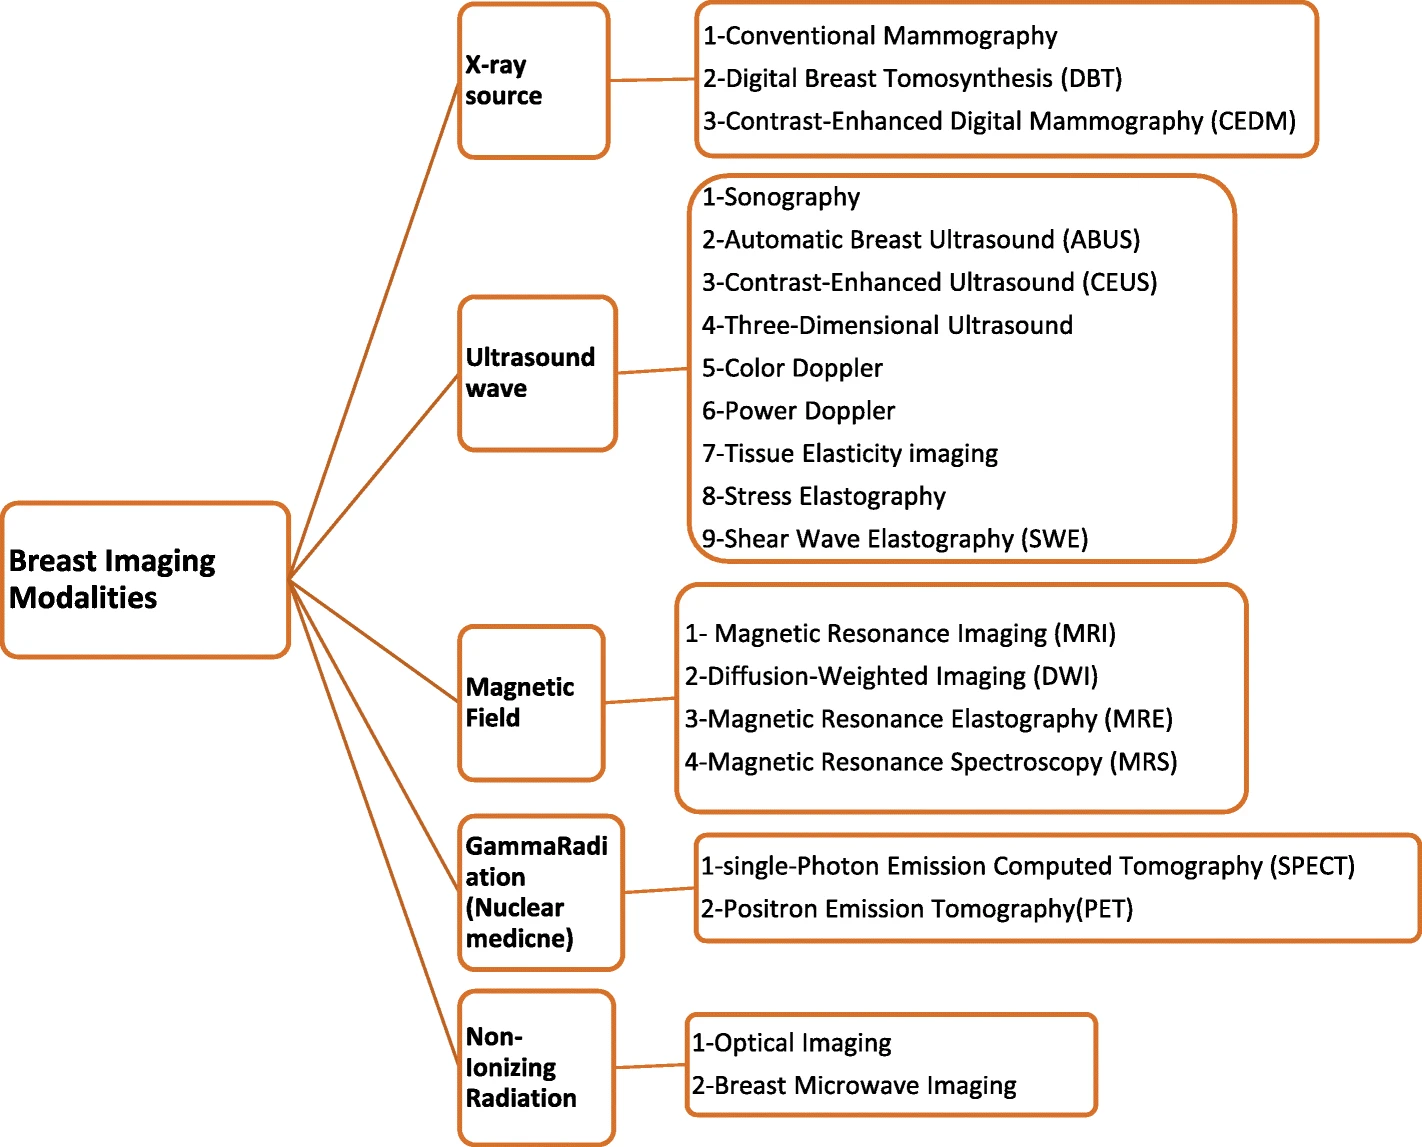
\includegraphics[width=0.75\linewidth]{reports//assets/medical_imaging.png}
    \caption[Resumen de modalidades de imagen mamaria]{Resumen de las modalidades de imagen mamaria clasificadas según el tipo de principio físico utilizado, incluyendo rayos X, ultrasonido, campo magnético, radiación gamma y técnicas no ionizantes \cite{iranmakani_review_2020}.}
    \label{fig:breast_cancer_medical}
\end{figure}

\subsection{Mamografía con rayos X}

En este trabajo, se emplearán imágenes de mamografía con rayos X como entrada para nuestro modelo, con el fin de inferir el subtipo molecular del cáncer de mama. Como técnica estándar en los programas de cribado poblacional, la mamografía con rayos X fue desarrollada específicamente para examinar la mama y otros tejidos blandos. El procedimiento se realiza utilizando un dispositivo médico especializado conocido como unidad o máquina de mamografía. Durante el examen, la mama se coloca sobre una placa de soporte plana y se comprime suavemente con una paleta. Luego, se emite un breve pulso de rayos X a través de la mama hacia un detector en el lado opuesto, que captura imágenes detalladas para su análisis (Figura \ref{fig:mammography}).

\begin{figure}[h!]
    \centering
    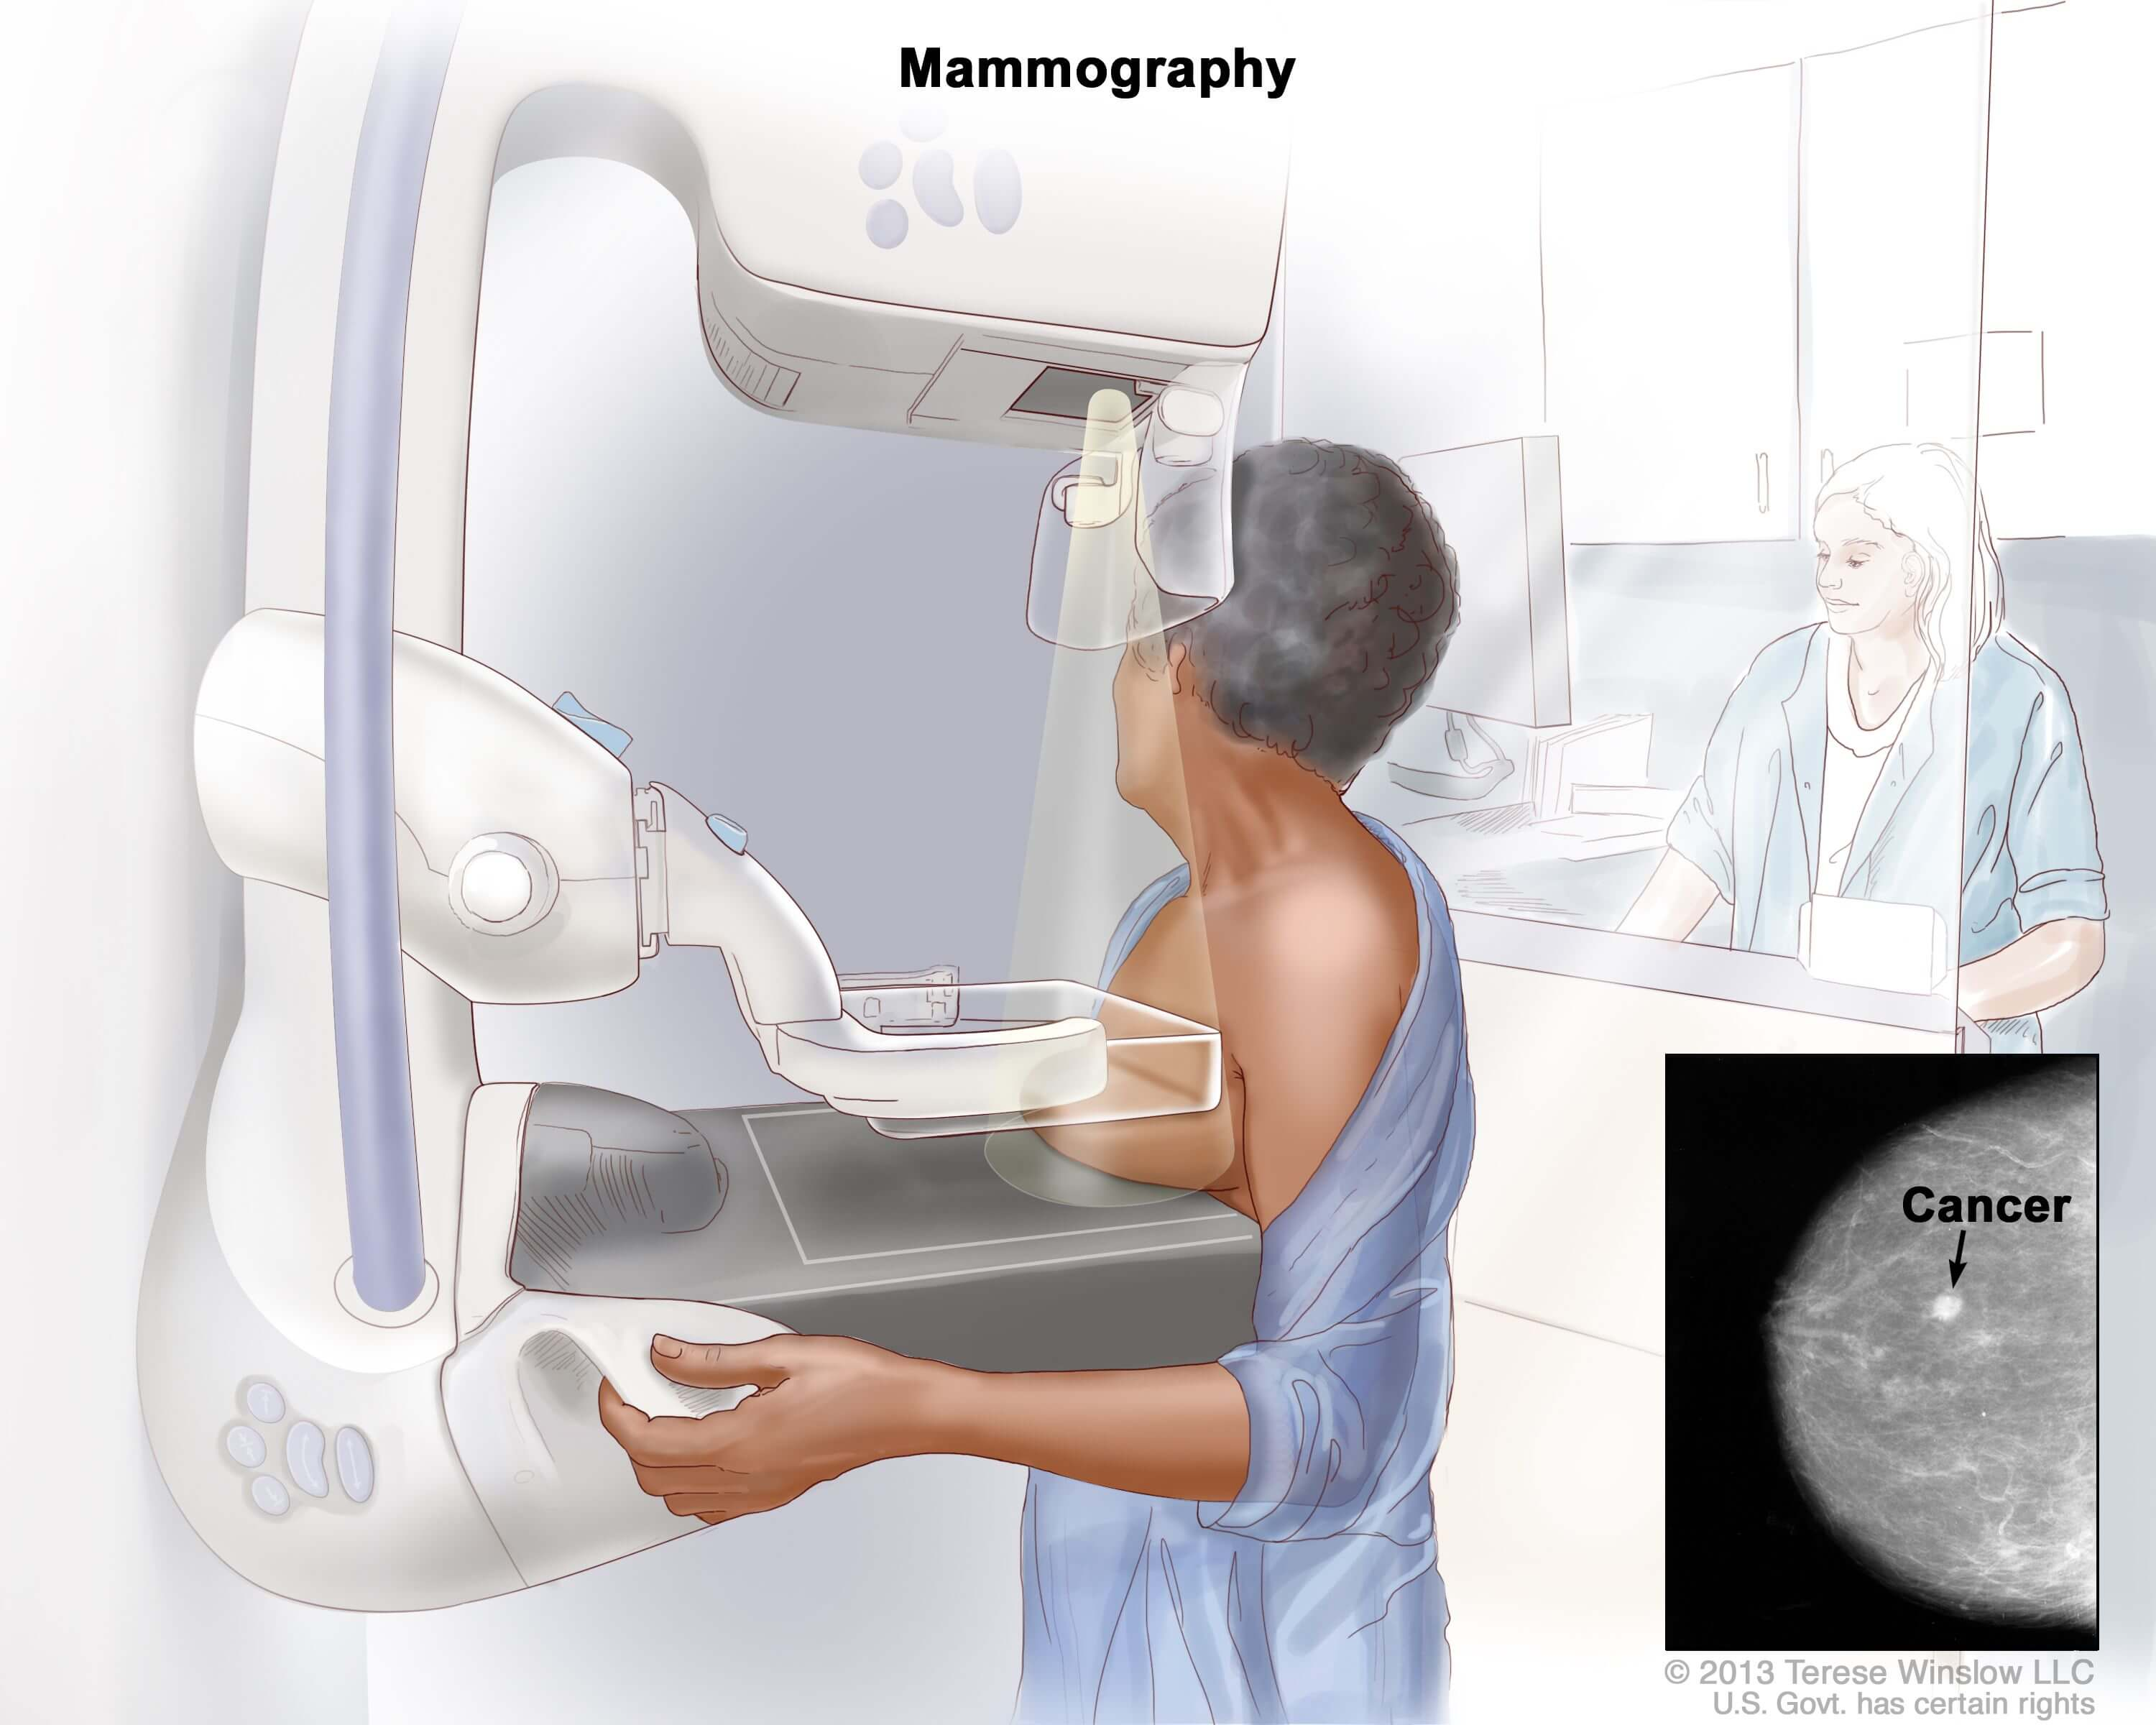
\includegraphics[width=0.45\linewidth]{reports//assets/mammography.jpg}
    \caption[Procedimiento tradicional de mamografía]{Ilustración que muestra el procedimiento tradicional de mamografía \cite{nihDefinitionMammogramNCI2011}.}
    \label{fig:mammography}
\end{figure}

Por lo general, cada mama se imagen mediante dos proyecciones estándar para asegurar la visualización del tejido:

\begin{itemize}
    \item \textbf{Proyección cráneo-caudal (CC)}: La vista CC se obtiene desde arriba de la mama (de la cabeza a los pies), proporcionando una perspectiva superior (0º) que permite una mayor visualización del tejido mamario posterior y superior. Esta vista es especialmente eficaz para identificar si las anomalías se encuentran medial o lateral al pezón \cite{noauthor_guide_nodate}.
    \item \textbf{Proyección medio-lateral oblicua (MLO)}: En la vista MLO, la mama se comprime en un ángulo oblicuo (generalmente alrededor de 45º), permitiendo cubrir prácticamente todo el tejido mamario \cite{noauthor_guide_nodate}. Esta vista es particularmente valiosa porque incluye la cola axilar y una porción significativa del músculo pectoral mayor, áreas donde se encuentra un porcentaje considerable (entre el 30\% y el 40\%) de los cánceres de mama \cite{aljarrah_trends_2014, noauthor_breast_2015}.
\end{itemize}

\begin{figure}[h!]
    \centering
    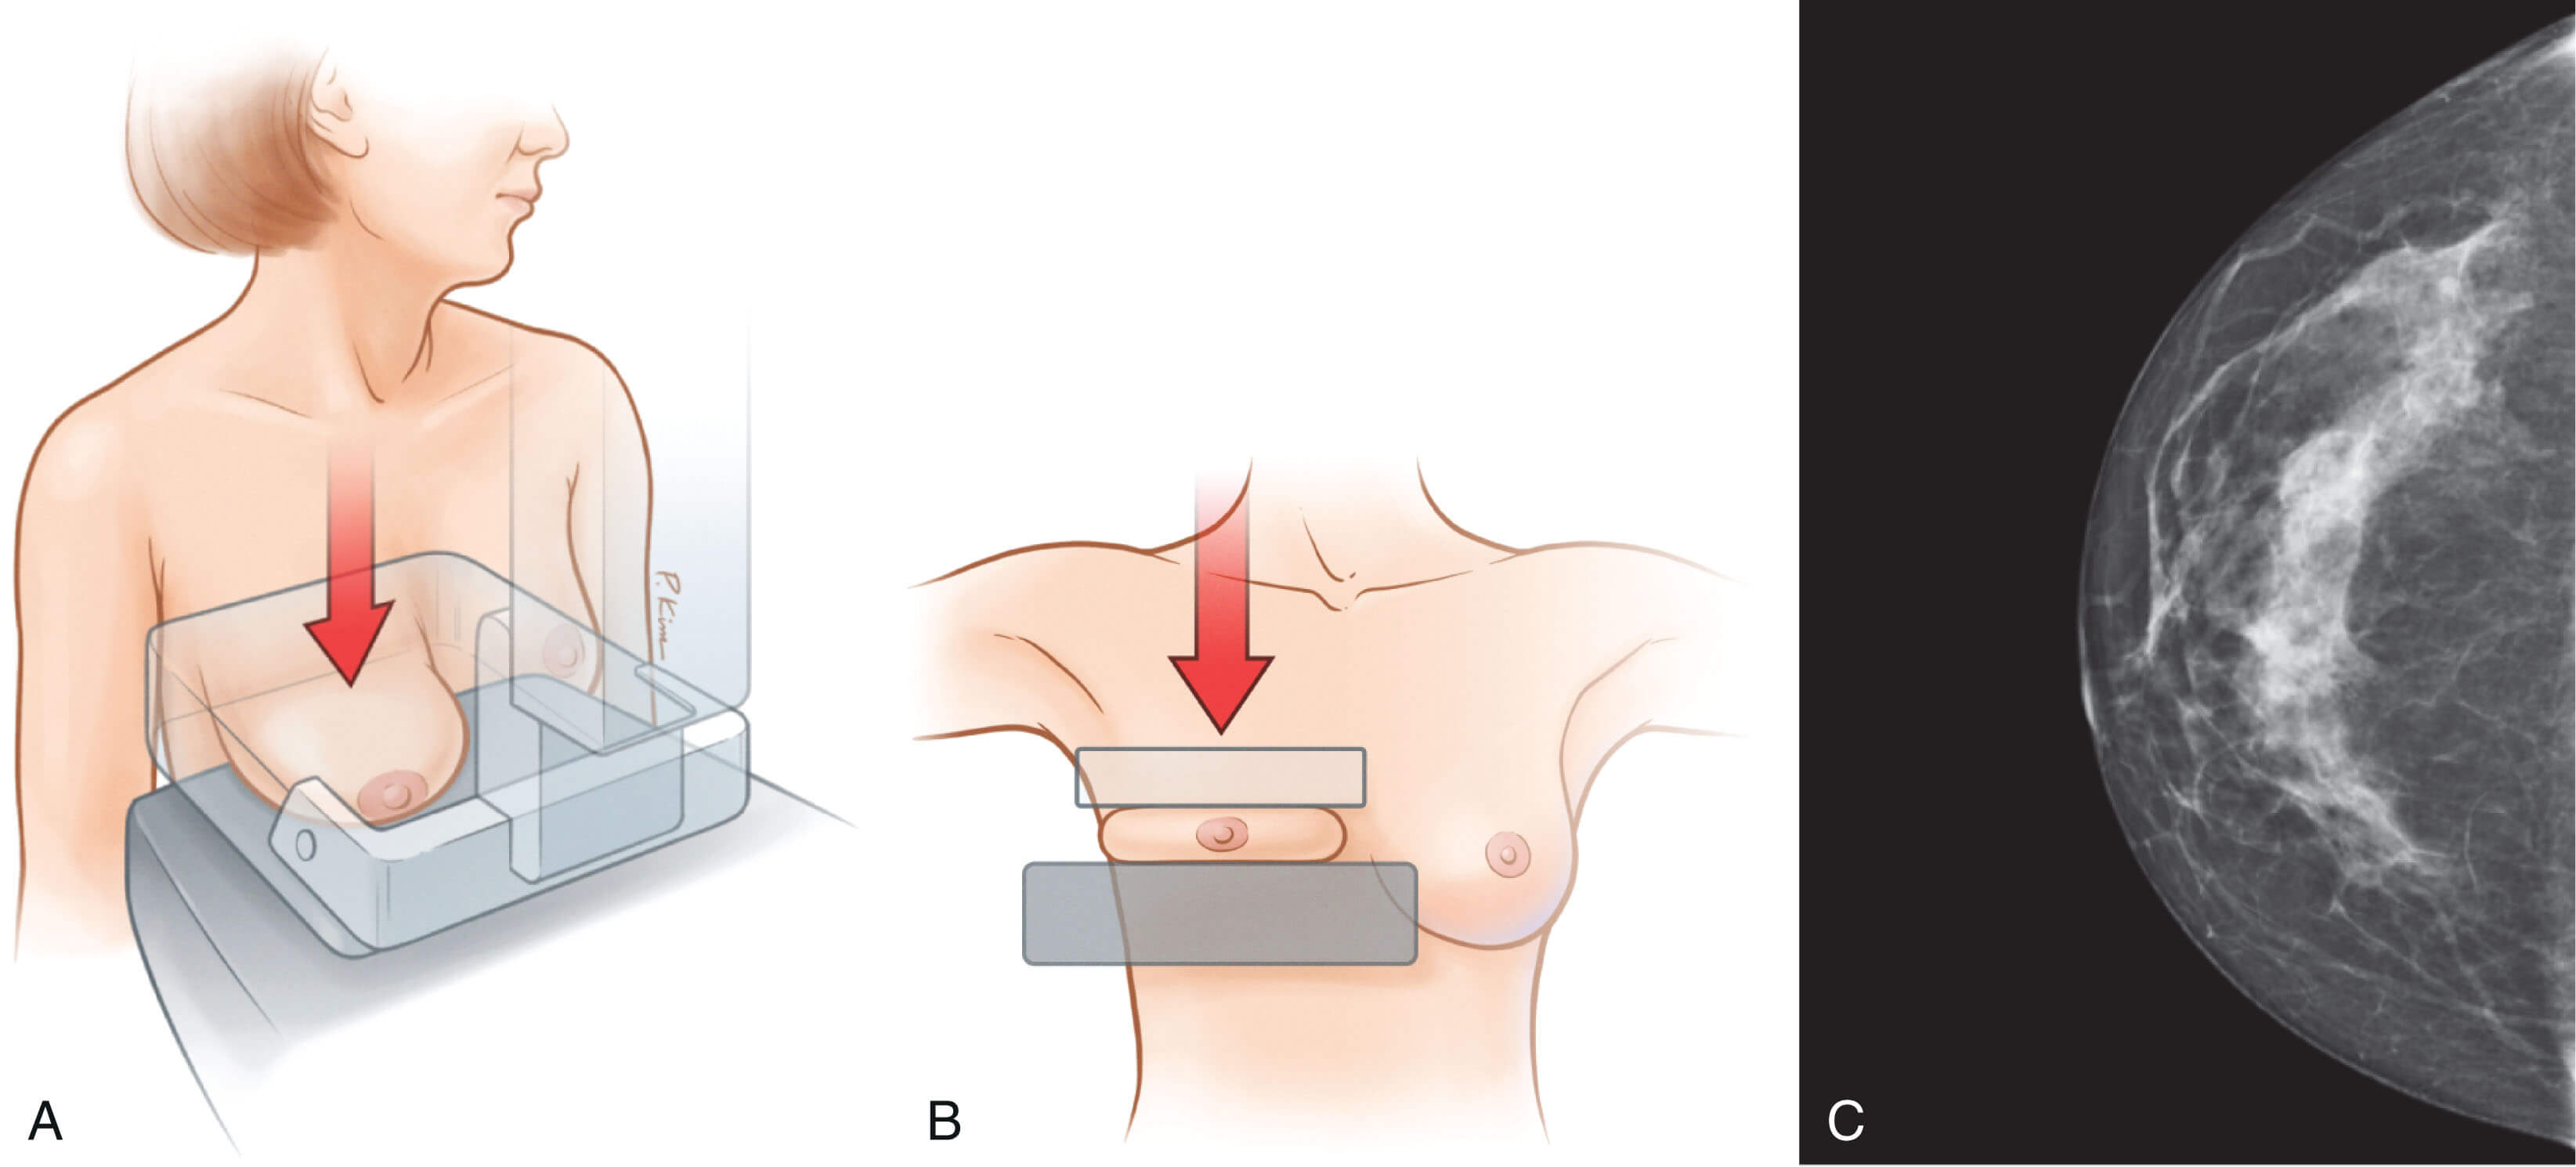
\includegraphics[width=0.6\linewidth]{reports//assets/cc_view.jpg}
    \caption[Procedimiento de adquisición de la vista CC]{Ilustración de la adquisición de la vista CC: (a) La mama se coloca horizontalmente sobre el detector y se comprime con una paleta. (b) Se aplica compresión desde arriba para obtener la proyección de rayos X. (c) Imagen resultante de la mamografía (vista CC) \cite{imaging_introduction_2022}. }
    \label{fig:cc_view}
\end{figure}

\begin{figure}[h!]
    \centering
    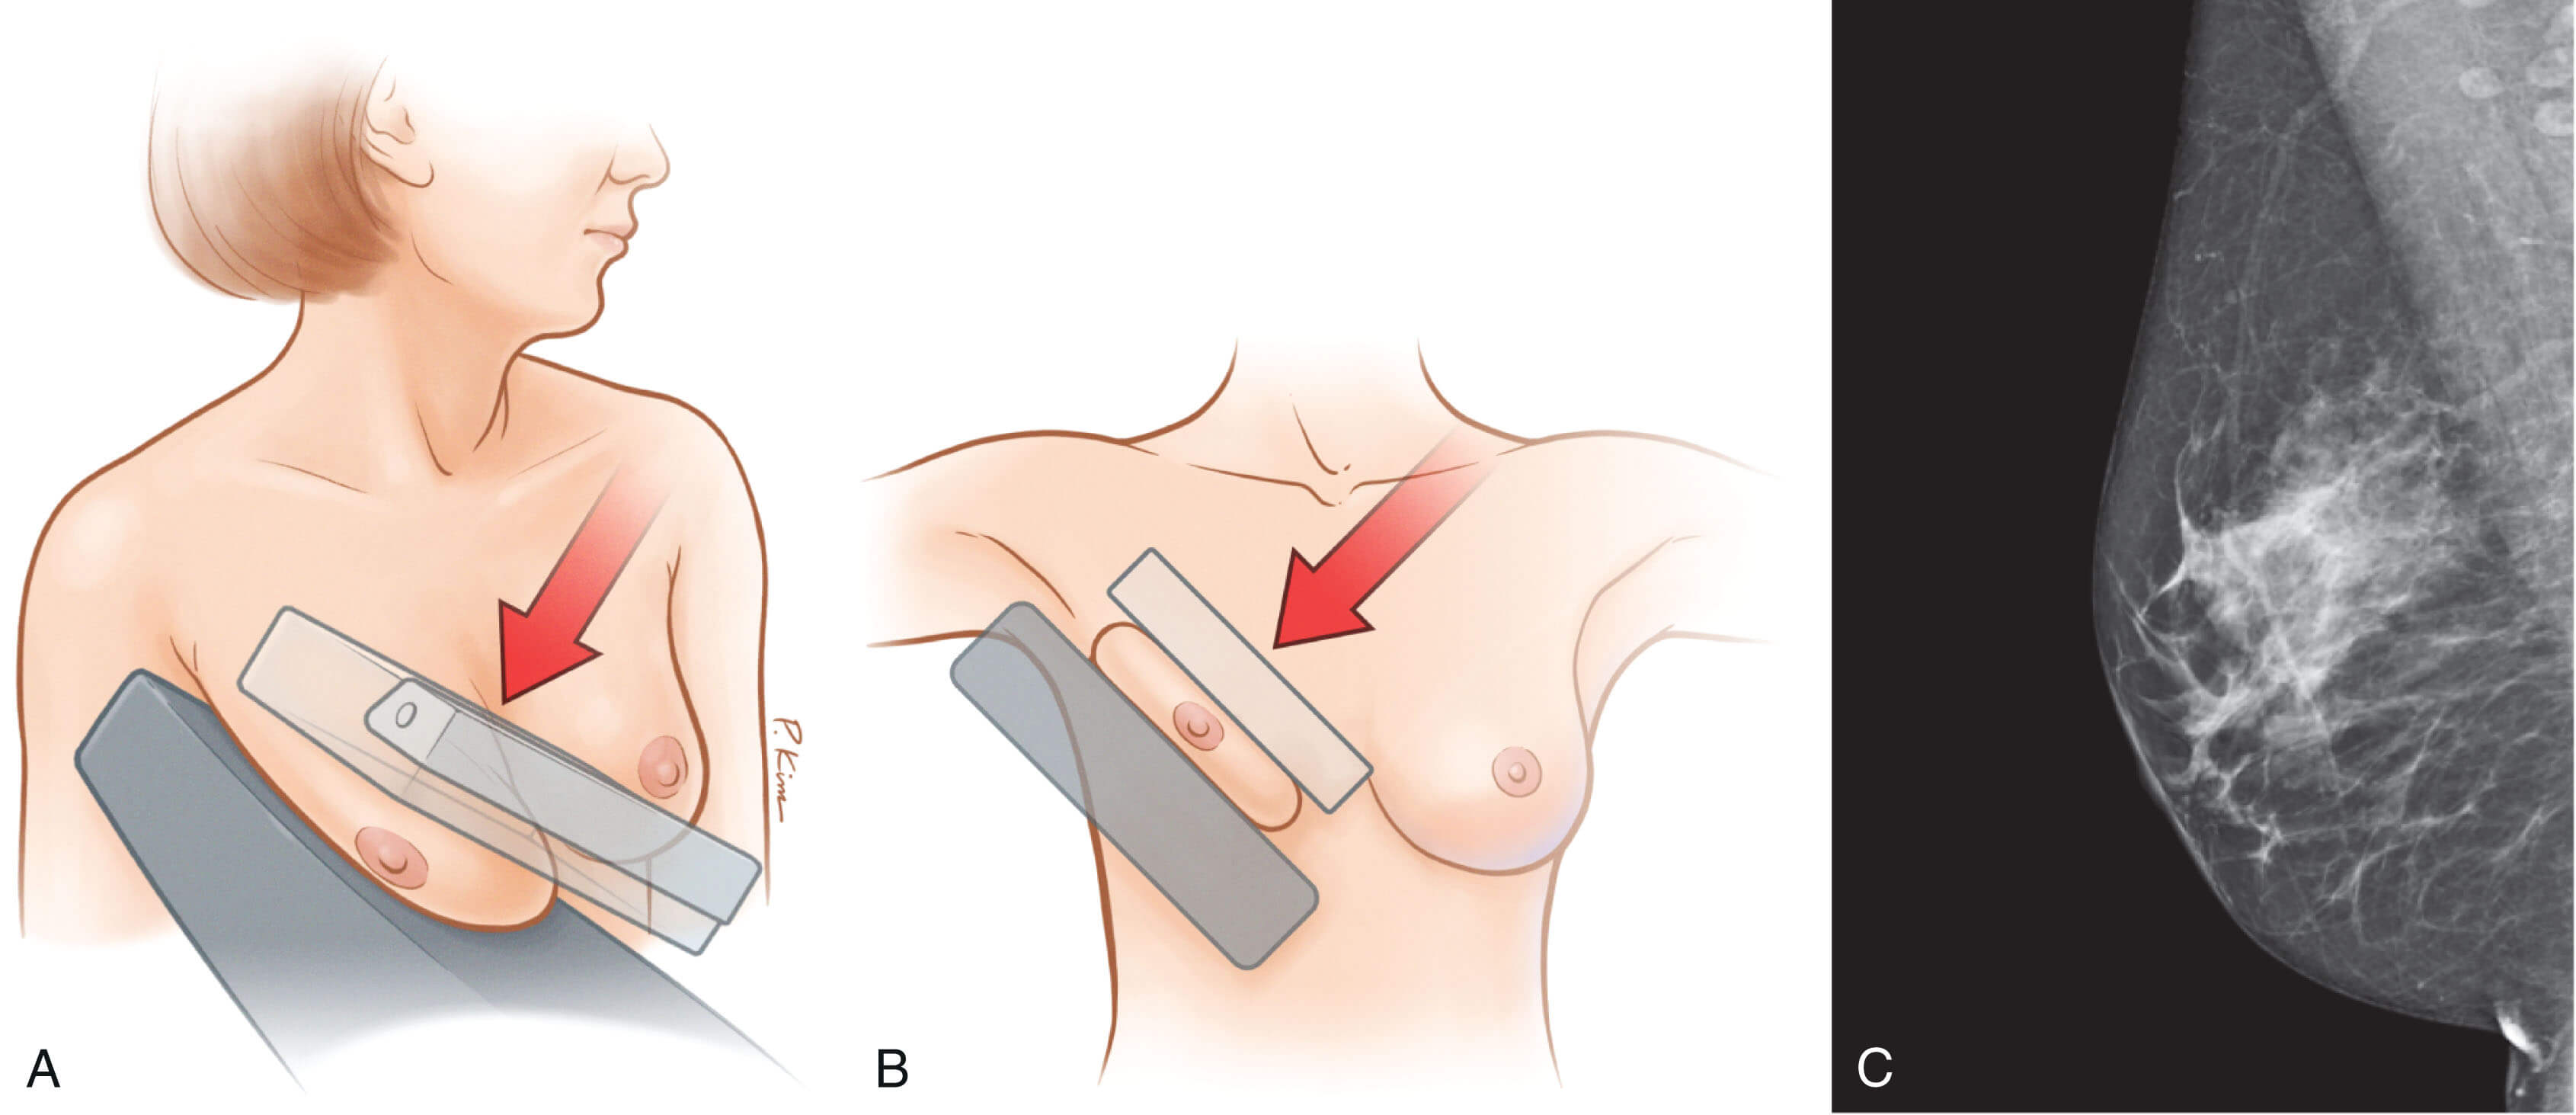
\includegraphics[width=0.6\linewidth]{reports//assets/mlo_view.jpg}
    \caption[Procedimiento de adquisición de la vista MLO]{Ilustración de la adquisición de la vista MLO: (a) La mama se posiciona en un ángulo oblicuo sobre el detector y se comprime con una paleta. (b) La compresión se aplica desde la parte superior interna hacia la parte inferior externa para obtener la proyección oblicua de rayos X. (c) Imagen resultante de la mamografía (vista MLO) \cite{imaging_introduction_2022}.}
    \label{fig:mlo_view}
\end{figure}


Las unidades modernas de mamografía pueden ser analógicas o digitales, siendo la mamografía digital la tecnología más utilizada y preferida actualmente en la práctica clínica \cite{ltd_mammography_2025, noauthor_mammography_nodate}. Los sistemas digitales ofrecen ventajas significativas sobre sus equivalentes analógicos, incluyendo adquisición inmediata de imágenes, mayor calidad de imagen y mayor facilidad para el almacenamiento y recuperación de las mismas.

Estos avances tecnológicos han fortalecido aún más el papel de la mamografía en la atención clínica. El uso de la mamografía con rayos X permite identificar cánceres de mama, tumores benignos y quistes antes de que sean palpables, detectando a menudo tumores en una etapa mucho más temprana que el examen físico por sí solo \cite{staff_what_2025}. Como resultado, esta técnica se emplea no solo para el cribado rutinario en mujeres asintomáticas, sino también para el diagnóstico de cáncer de mama tras la detección de un bulto u otros síntomas, así como para la vigilancia continua después de un diagnóstico de cáncer de mama.


\subsection{Otras modalidades}

\textbf{Ecografía mamaria}

La ecografía mamaria es una técnica ampliamente utilizada para el análisis de la mama que emplea un dispositivo manual llamado transductor\footnote{Dispositivo que emite ondas sonoras que rebotan en los tejidos del cuerpo, recibe los ecos y transforma las señales en imágenes.} para producir imágenes en tiempo real del tejido mamario interno mediante la emisión de ondas sonoras de alta frecuencia (Figura~\ref{fig:breast_ultrasound_comparison}).

A diferencia de la mamografía, la ecografía no utiliza radiación ionizante, lo que la convierte en una opción segura y no invasiva para pacientes de todas las edades. Esta modalidad resulta especialmente valiosa para evaluar nódulos palpables, distinguir entre masas sólidas y quísticas, y caracterizar más detalladamente lesiones detectadas en la mamografía, especialmente en mujeres con tejido mamario denso, donde la mamografía puede ser menos sensible \cite{gokhale_ultrasound_2009}.

Sin embargo, es importante tener en cuenta que la precisión y calidad de los exámenes ecográficos dependen en gran medida de la habilidad y experiencia del operador. Además, en comparación con la mamografía, la ecografía es menos eficaz para diferenciar entre lesiones benignas y malignas, lo que puede dar lugar a un mayor número de procedimientos de seguimiento.

\begin{figure}[h!]
	\centering
	\begin{subfigure}[c]{0.45\textwidth}
		\centering
		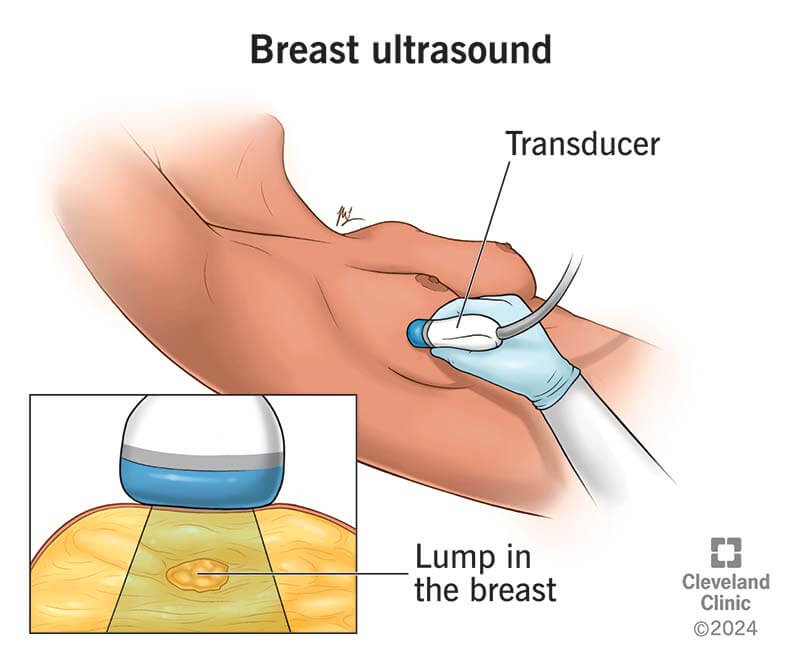
\includegraphics[width=\textwidth]{reports/assets/breast_ultrasound.jpg}
            \caption{}
		\label{fig:breast_ultrasound}
	\end{subfigure}
	\begin{subfigure}[c]{0.45\textwidth}
		\centering
		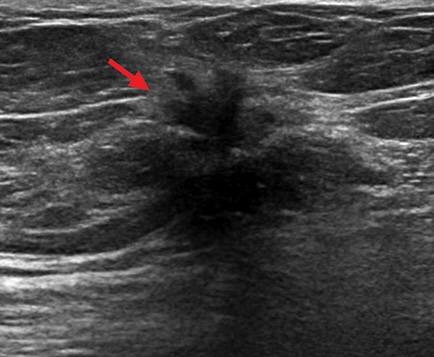
\includegraphics[width=\textwidth]{reports/assets/ultrasound.jpg}
            \caption{}
		\label{fig:ultrasound}
	\end{subfigure}
	\caption[Procedimiento y ejemplo de ecografía mamaria]{(a) Representación de la ecografía mamaria \cite{macauley_start--finish_2022}. (b) Ejemplo de ecografía mamaria que muestra una masa irregular, de color gris oscuro y espiculada, altamente sospechosa de cáncer \cite{noauthor_breast_nodate}.}
\label{fig:breast_ultrasound_comparison}
\end{figure}


\textbf{Resonancia Magnética (RM)}

La RM es un procedimiento de imagen no invasivo que utiliza campos magnéticos intensos y ondas de radio para producir una serie de imágenes altamente detalladas de las estructuras internas del cuerpo. En la imagen mamaria, la RM opera bajo el mismo principio fundamental y suele emplearse junto a otras modalidades de imagen para detectar cáncer de mama u otras anomalías \cite{nih_definition_2011}.

La RM mamaria es especialmente valiosa para mujeres con alto riesgo de desarrollar cáncer de mama, como aquellas con mutaciones genéticas o antecedentes familiares importantes de la enfermedad. Esto se debe a su alta sensibilidad, con tasas de detección superiores al 90\%, lo que la convierte en la modalidad de imagen más sensible para identificar cáncer de mama \cite{radswiki_breast_nodate}.

A pesar de estas ventajas, la RM es más costosa y menos accesible que la mamografía o la ecografía. Su alta sensibilidad puede conducir, en ocasiones, a un mayor número de falsos positivos, lo que resulta en pruebas adicionales de seguimiento. Además, la interpretación precisa de la RM mamaria requiere formación y experiencia especializadas \cite{noauthor_technical_nodate}.

\begin{figure}
    \centering
    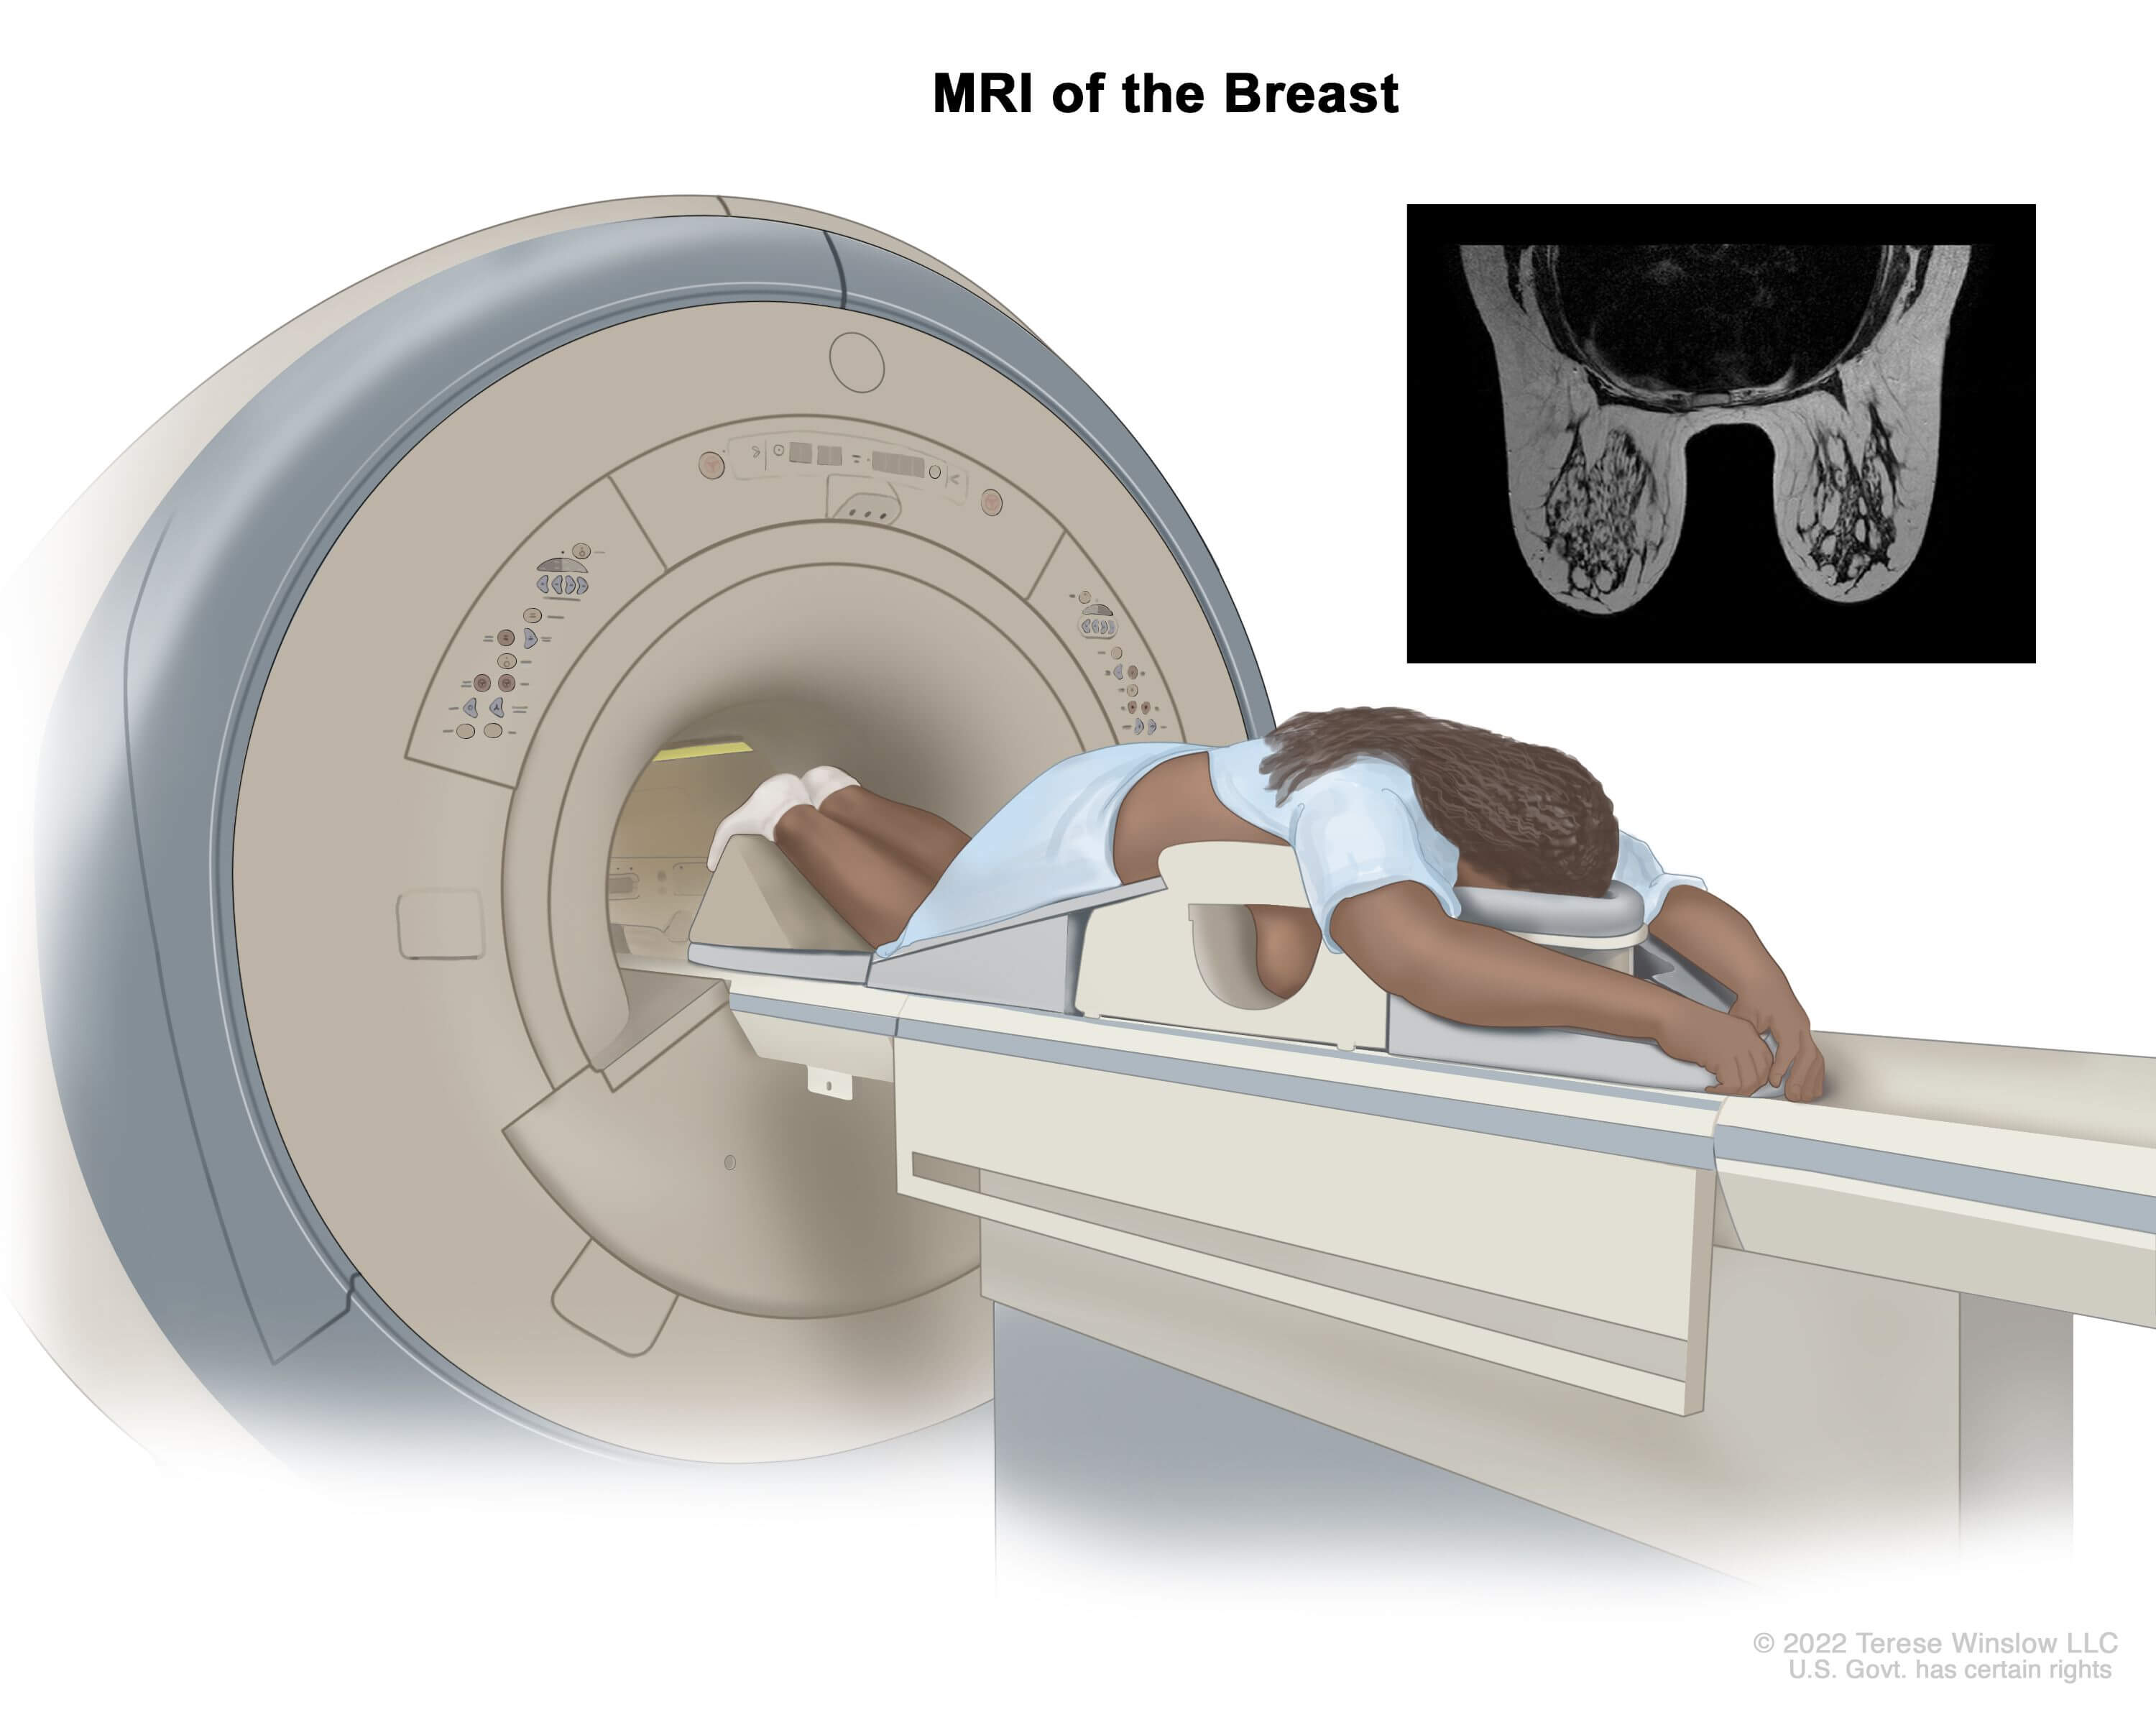
\includegraphics[width=0.5\linewidth]{reports//assets/breast_mri.jpg}
    \caption[Procedimiento de RM mamaria]{Ilustración de un procedimiento de RM mamaria. La paciente se coloca en decúbito prono sobre una bobina dedicada para la mama, permitiendo una imagen óptima del tejido mamario \cite{nih_definition_2011}.}
    \label{fig:breast_mri}
\end{figure}

\section{Cribado del cáncer}

El cribado del cáncer es el proceso de utilizar pruebas para buscar cáncer o cambios precancerosos en las personas, principalmente dirigido a aquellas que no presentan síntomas de la enfermedad. El objetivo es detectar el cáncer en una etapa temprana, cuando el tratamiento tiene más probabilidades de éxito y antes de que aparezcan los síntomas \cite{noauthor_cancer_2010}.

Existen diferentes tipos de pruebas de cribado que pueden emplearse en el proceso según las necesidades del sujeto. Estas pueden incluir exámenes físicos y revisión de la historia clínica, pruebas de laboratorio, procedimientos de imagen y pruebas genéticas \cite{noauthor_cancer_2010}. En el contexto del cáncer de mama, la mamografía con rayos X es la herramienta estándar de cribado. Como se mencionó anteriormente, se trata de una técnica ampliamente disponible, no invasiva y rentable, y se ha demostrado que permite detectar tumores hasta dos años antes de que sean palpables o provoquen síntomas \cite{cancer_que_2023}.

\subsection{Descripción general del proceso}

El proceso general de cribado mamario es muy similar en todo el mundo en sus pasos principales, aunque ciertos aspectos, como la edad de inicio, la frecuencia del cribado y la tecnología utilizada, pueden variar de un país a otro. En España, el programa de cribado de cáncer de mama comenzó en 1990 y se realiza únicamente en mujeres entre 50 y 69 años, utilizando mamografías bienales\footnote{Cada dos años} \cite{noauthor_ministerio_nodate}. Los siguientes pasos son los pasos fundamentales del cribado de cáncer de mama:

\begin{enumerate}
    \item \textbf{Invitación}: Se invita a participar a las mujeres elegibles (según la edad y, en ocasiones, factores de riesgo), ya sea a través de programas nacionales organizados o mediante los proveedores de atención sanitaria.
    \item \textbf{Prueba de cribado}: Se realiza la prueba de cribado, habitualmente una mamografía, que puede complementarse con otras pruebas. Por ejemplo, en España también se recomienda la ecografía \cite{noauthor_map_nodate}.
    \item \textbf{Revisión de imágenes}: Los radiólogos revisan las mamografías en busca de signos de cáncer, como masas o microcalcificaciones.
    \item \textbf{Notificación de resultados}: Se informa a las mujeres de sus resultados. Aquellas con hallazgos anómalos son citadas para pruebas adicionales.
    \item \textbf{Seguimiento}: Si se detectan anomalías, se realizan procedimientos diagnósticos adicionales, como estudios de imagen complementarios o biopsias, para confirmar o descartar el cáncer.
\end{enumerate}

En esta etapa, técnicas no invasivas, como las investigadas en este trabajo, pueden contribuir a mejorar los resultados diagnósticos y ofrecer información más detallada. En concreto, en el contexto de la clasificación de subtipos moleculares, disponer de una herramienta de este tipo proporcionaría información adicional en casos con hallazgos anómalos o cánceres confirmados. Esto podría traducirse en un mejor pronóstico y ayudar a guiar la toma de decisiones clínicas, reduciendo potencialmente la necesidad de procedimientos invasivos adicionales como las biopsias.


\subsection{Técnicas de biopsia}

Cuando las pruebas de imagen u otros exámenes de cribado detectan anomalías sugestivas de cáncer de mama, normalmente se requiere una biopsia para obtener un diagnóstico definitivo. La biopsia mamaria consiste en extraer una pequeña muestra de tejido del área sospechosa, que posteriormente es examinada al microscopio por un patólogo \cite{DefinitionBiopsyNCI2011}. Este paso es crucial no solo para confirmar la presencia de cáncer, sino también para determinar su tipo, grado y, cada vez más, sus características moleculares.

\textbf{Clasificación}

Existen varias técnicas de biopsia comúnmente empleadas para el diagnóstico y caracterización de lesiones mamarias, entre las que se incluyen:

\begin{itemize}
    \item \textbf{Aspiración con aguja fina (AAF)}: Procedimiento mínimamente invasivo que utiliza una aguja fina y hueca para extraer células o líquido de una zona sospechosa. Suele realizarse cuando la lesión probablemente es un quiste\footnote{Saco lleno de líquido}. La AAF es rápida, rentable y generalmente bien tolerada, ofreciendo alta precisión diagnóstica cuando se realiza correctamente. Sin embargo, puede aportar información limitada sobre la estructura tisular y, en ocasiones, arrojar resultados no concluyentes, requiriendo una evaluación adicional mediante biopsia con aguja gruesa o quirúrgica \cite{noauthor_fine_nodate, silva_breast_2023}.
    
    \item \textbf{Biopsia con aguja gruesa (BAG)}: Esta técnica emplea una aguja hueca de mayor calibre para obtener pequeños cilindros (core) de tejido, habitualmente bajo guía por imagen \cite{CoreNeedleBiopsy, silva_breast_2023}. La BAG proporciona una muestra tisular más grande, permitiendo un diagnóstico histológico preciso y la evaluación de marcadores moleculares, ambos esenciales para la subtipificación molecular. Se considera el enfoque diagnóstico estándar debido a su alta concordancia con las muestras quirúrgicas para biomarcadores clave como RE, RP, HER2 y Ki67 \cite{jeong_analysis_2020}.
    
    \item \textbf{Biopsia asistida por vacío (BAV)}: La BAV utiliza un dispositivo accionado por vacío para recoger múltiples muestras de tejido a través de una sola punción, generalmente guiada por imagen estereotáctica\footnote{Técnica o procedimiento quirúrgico que utiliza un sistema de coordenadas tridimensional para localizar y dirigir con precisión una zona específica.} o ecografía. Es especialmente eficaz para el muestreo de microcalcificaciones o lesiones pequeñas detectadas mediante mamografía y proporciona muestras tisulares de mayor tamaño, reduciendo así el error de muestreo. Este método es fiable, bien tolerado y, en ocasiones, puede evitar la necesidad de una biopsia quirúrgica, especialmente en lesiones benignas \cite{park_vacuum-assisted_2014}.
    
    \item \textbf{Biopsia quirúrgica}: Cuando las técnicas con aguja no son concluyentes o no son factibles, puede realizarse una biopsia quirúrgica para extirpar parte o la totalidad del tejido sospechoso. Aunque proporciona la muestra tisular más completa, también es más invasiva y costosa, y generalmente se reserva para casos en los que los métodos menos invasivos no permiten un diagnóstico definitivo \cite{silva_breast_2023}.
\end{itemize}

\textbf{Limitaciones}

La elección de la técnica de biopsia depende de factores como el tamaño de la lesión, su localización, las características en imagen y consideraciones específicas de la paciente. Aunque la biopsia sigue siendo el estándar de oro para el diagnóstico de cáncer, está asociada a varias limitaciones importantes, entre ellas:

\begin{itemize}
    \item \textbf{Invasividad}: El procedimiento puede causar molestias y conlleva un riesgo potencial de infección o sangrado, especialmente cuando los tumores se encuentran en zonas de difícil acceso \cite{amino_pros_2024}.
    \item \textbf{Barreras logísticas}: En entornos con recursos limitados, la falta de personal capacitado y la necesidad de que las pacientes se desplacen largas distancias para recibir atención pueden dificultar el diagnóstico y tratamiento oportunos \cite{silva_breast_2023}.
    \item \textbf{Resultados no concluyentes}: Si no es realizada por personal experimentado, la biopsia puede arrojar muestras insuficientes o no diagnósticas, aumentando la carga y el malestar de la paciente debido a la necesidad de repetir el procedimiento.
\end{itemize}

Dadas estas limitaciones, existe una clara necesidad de desarrollar enfoques diagnósticos no invasivos. Dichas técnicas podrían facilitar una intervención más temprana, reducir la dependencia de la toma de muestras tisulares y mejorar el acceso a un diagnóstico oportuno y preciso, especialmente en contextos donde la biopsia no es factible.



\chapter{Revisión tecnológica}

Esta sección explora las definiciones y estructuras modernas de los modelos de IA, así como su uso en la medicina actual y específicamente en la imagen médica.

\section{Inteligencia Artificial}

La Inteligencia Artificial (IA) se refiere a un conjunto de tecnologías que permiten a los ordenadores y máquinas imitar la inteligencia humana, incluyendo el aprendizaje, la resolución de problemas y la toma de decisiones con distintos niveles de creatividad y autonomía \cite{colestrykerWhatArtificialIntelligence2024}. Las raíces conceptuales de la IA se remontan a las décadas de 1940 y 1950, cuando pioneros como Alan Turing exploraron la idea de que las máquinas pudieran simular el pensamiento humano. El trabajo de Turing, incluyendo el influyente “Test de Turing” y su artículo de 1950, sentó las bases del campo \cite{turing_icomputing_1950}. La IA se estableció formalmente como disciplina en 1956 en la Conferencia de Dartmouth, donde el término “inteligencia artificial” fue introducido por John McCarthy, Marvin Minsky, Nathaniel Rochester y Claude Shannon \cite{filipsson_evolution_2024}. La Figura \ref{fig:ai_timeline} resume la evolución de la IA a lo largo de las décadas y destaca los hitos clave en su desarrollo.

\begin{figure}[h!]
\centering
\begin{chronology}*[5]{1949}{2025}{\textwidth}
  \event{1950}{\footnotesize Propuesta del test de Turing}
  \event{1956}{\footnotesize Dartmouth: acuñación del término \textit{IA}}
  \event{1965}{\footnotesize Sistemas expertos}
  \event[1974]{1980}{\footnotesize Primer invierno de la IA}
  \event{1986}{\footnotesize Introducción del backpropagation}
  \event[1987]{1993}{\footnotesize Segundo invierno de la IA}
  \event{2012}{\footnotesize Revolución del aprendizaje profundo}
  \event{2020}{\footnotesize Vision Transformers}
\end{chronology}
\caption[Línea temporal de la IA]{Línea temporal condensada de los principales hitos de la IA}
\label{fig:ai_timeline}
\end{figure}

\subsection{IA clásica}

Los primeros años de la inteligencia artificial se centraron en la programación explícita y los sistemas basados en reglas, conocidos como sistemas expertos, que buscaban imitar la resolución de problemas humana. Ejemplos notables incluyen Dendral, utilizado para el análisis de estructuras químicas, y Mycin, desarrollado para diagnosticar infecciones bacterianas y sugerir tratamientos. Estos sistemas, desarrollados en las décadas de 1960 y 1970, demostraron el potencial de la IA en campos como la medicina y la investigación científica \cite{filipsson_evolution_2024}.

Sin embargo, los enfoques basados en reglas pronto revelaron limitaciones significativas, como su incapacidad para adaptarse a nueva información o gestionar datos complejos y no estructurados. Combinado con recursos computacionales limitados y expectativas poco realistas, estos desafíos condujeron a periodos de estancamiento en la investigación en IA, conocidos como “inviernos de la IA”. El campo eventualmente resurgió a medida que los datos digitales se hicieron más accesibles y surgieron nuevos paradigmas de IA.

\subsection{Aprendizaje automático}

El Aprendizaje Automático (Machine Learning, ML) es una rama de la inteligencia artificial que permite a los ordenadores aprender a partir de datos y experiencia, lo que les permite reconocer patrones, hacer inferencias y predecir resultados sin necesidad de programación explícita basada en reglas \cite{noauthor_what_nodate}. Su rápido crecimiento ha sido impulsado por la explosión del big data, los avances en recursos computacionales y la disponibilidad de grandes conjuntos de datos anotados. El ML abarca varios paradigmas principales de aprendizaje:

\begin{itemize}
\item \textbf{Aprendizaje supervisado}: Los modelos se entrenan con datos etiquetados, donde cada entrada está emparejada con una salida conocida, lo que permite al modelo aprender la relación entre ambas \cite{jiang_supervised_2020}.
\item \textbf{Aprendizaje no supervisado}: Los modelos trabajan con datos no etiquetados, buscando descubrir patrones o estructuras ocultas dentro del conjunto de datos \cite{noauthor_unsupervised_nodate}.
\item \textbf{Aprendizaje por refuerzo}: Los modelos aprenden interactuando con un entorno, recibiendo retroalimentación en forma de recompensas o penalizaciones, y mejorando gradualmente sus estrategias de toma de decisiones \cite{ghasemi_introduction_2024}.
\end{itemize}

La adopción del ML ha tenido un impacto transformador en numerosas industrias. En el ámbito sanitario, los modelos de ML asisten actualmente en tareas que van desde el análisis automatizado de imágenes médicas hasta la recomendación personalizada de tratamientos. El rápido avance de las aplicaciones de ML, junto con la explosión de datos disponibles y las mejoras en hardware (como las GPU), allanaron el camino para el siguiente gran salto en IA: el aprendizaje profundo (Deep Learning, DL).

\subsection{Aprendizaje profundo}

El aprendizaje profundo (DL) es una especialización dentro del ML que utiliza redes neuronales artificiales (ANN) compuestas por múltiples capas para extraer automáticamente características complejas de grandes conjuntos de datos. Este enfoque ha permitido un rendimiento sin precedentes en campos como el análisis de imágenes, el reconocimiento de voz y el procesamiento del lenguaje natural \cite{holdsworthWhatDeepLearning2024}.

A diferencia de los métodos tradicionales de ML, que suelen depender de la ingeniería manual de características y están mejor adaptados a conjuntos de datos estructurados y de tamaño moderado, los modelos de DL sobresalen en el procesamiento de grandes cantidades de datos no estructurados, como imágenes, audio y texto. Estos modelos son capaces de aprender representaciones jerárquicas de manera autónoma directamente a partir de los datos brutos, reduciendo significativamente la intervención humana y mejorando tanto la escalabilidad como la precisión \cite{holdsworthWhatDeepLearning2024}. La Figura~\ref{fig:ai_overview} ilustra cómo el DL se integra en el contexto más amplio de la IA y el ML.

\begin{figure}[h!]
    \centering
    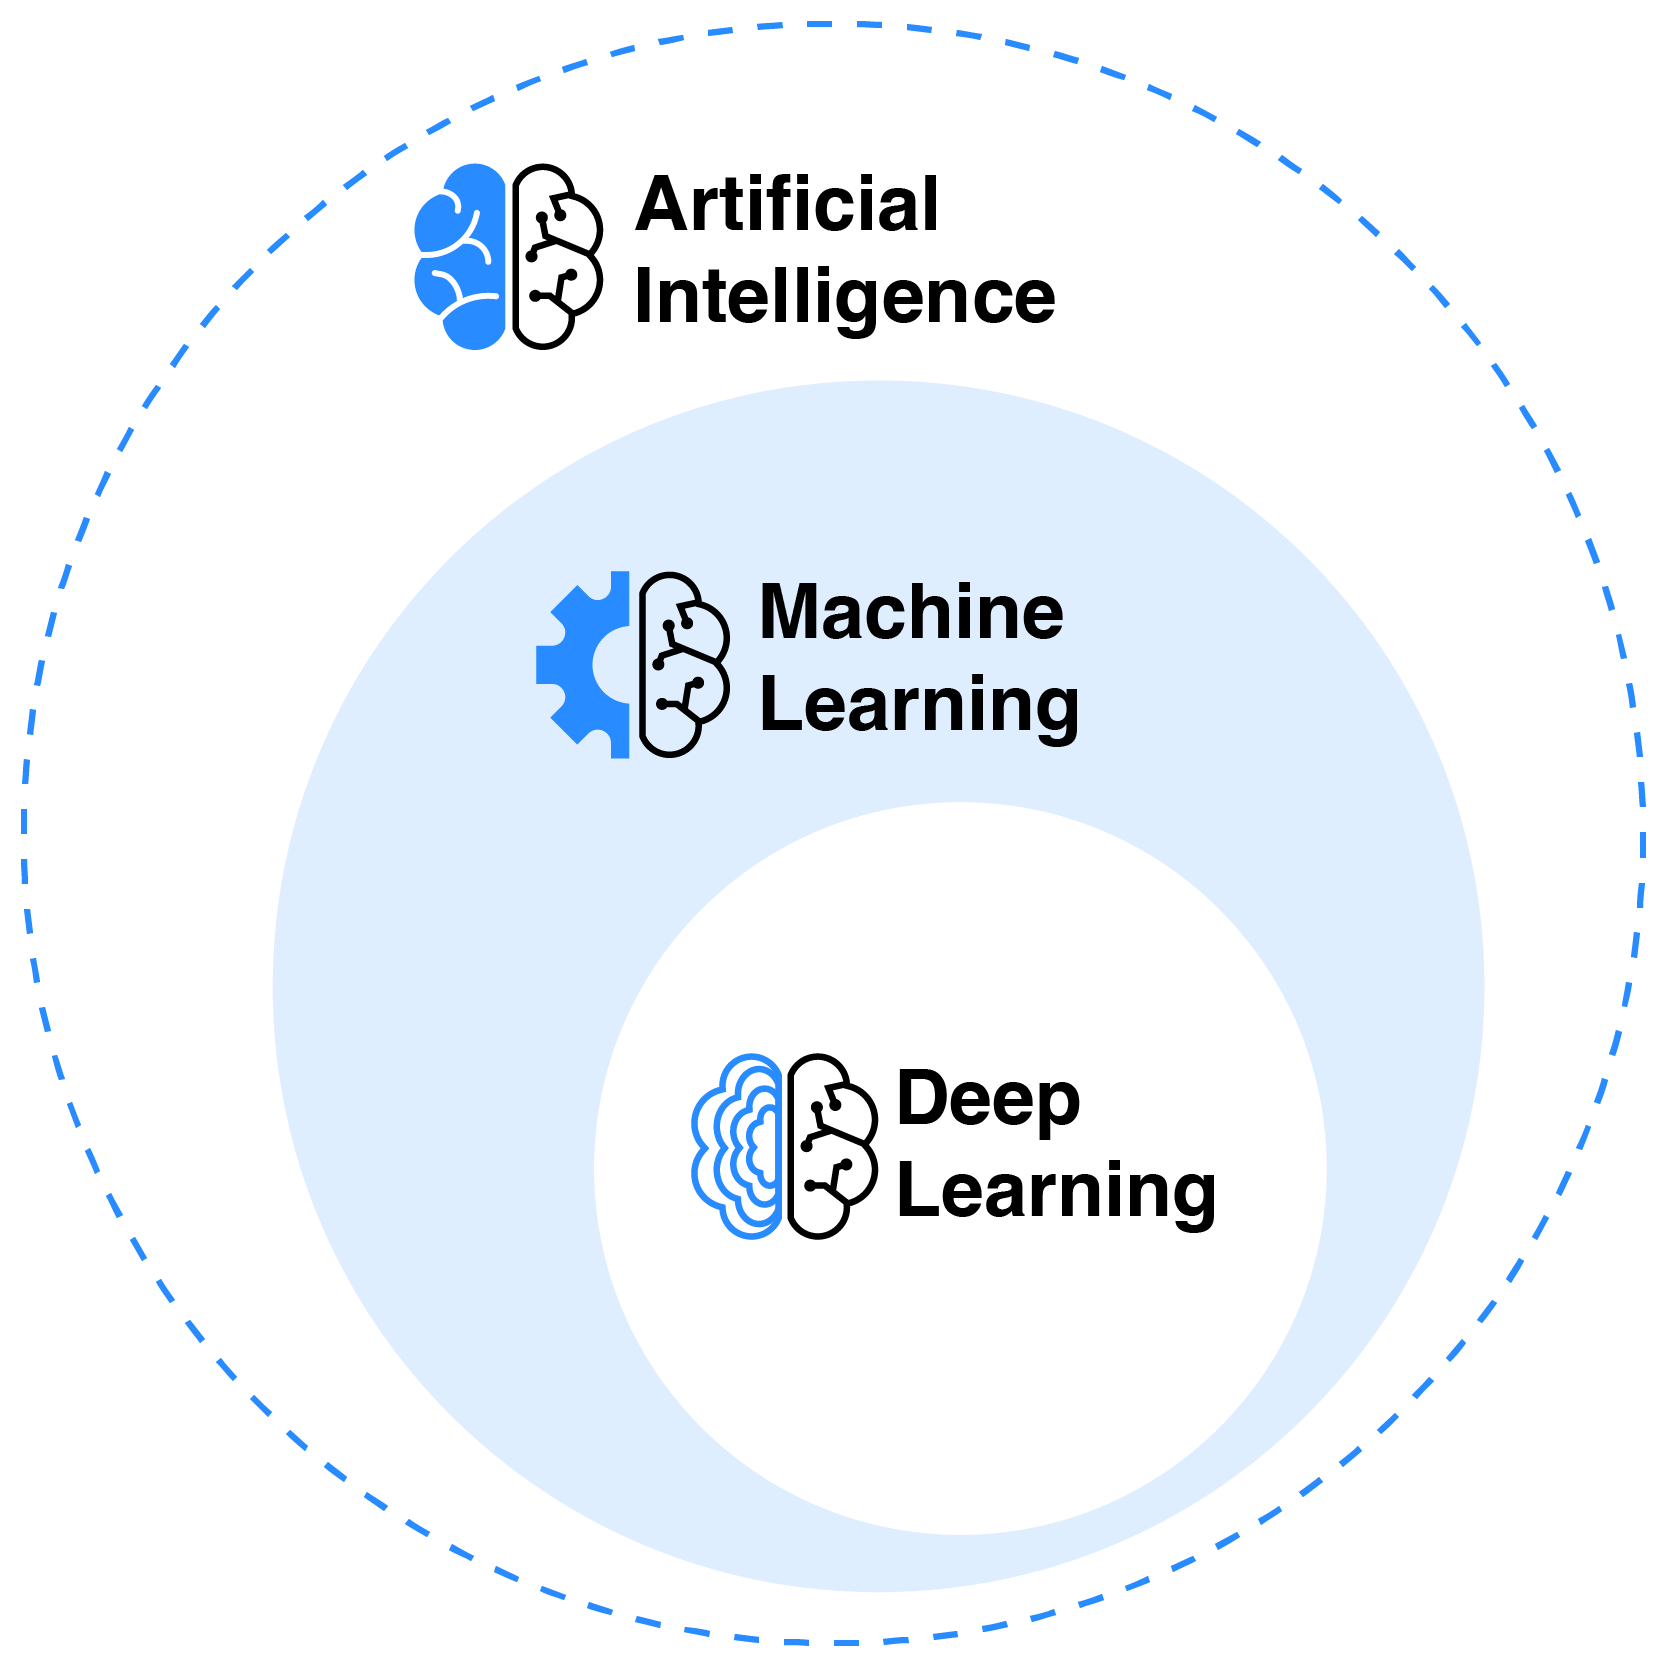
\includegraphics[width=0.5\linewidth]{reports//assets/ai.png}
    \caption[Resumen de subconjuntos de IA]{Resumen de los subconjuntos de IA \cite{nasaWhatArtificialIntelligence}.}
    \label{fig:ai_overview}
\end{figure}

\subsection{Aprendizaje profundo en imagen médica}

La llegada de las técnicas de DL ha transformado profundamente el campo de la imagen médica, permitiendo un análisis altamente preciso de datos visuales complejos en un amplio espectro de aplicaciones clínicas, incluyendo:

\begin{itemize}
    \item \textbf{Clasificación y detección de imágenes}: Los modelos de DL se entrenan para identificar y clasificar anomalías en imágenes radiológicas como radiografías, RM o mamografías, alcanzando a menudo un rendimiento a nivel experto.
    \item \textbf{Segmentación}: Las arquitecturas de DL facilitan la delimitación precisa de estructuras anatómicas y regiones patológicas, lo que es esencial para la planificación del tratamiento, el diagnóstico y el seguimiento de enfermedades.
    \item \textbf{Mejora y generación de imágenes}: El DL se emplea para mejorar la calidad de las imágenes (por ejemplo, reducción de ruido, superresolución) y para generar datos sintéticos destinados a la ampliación de conjuntos de datos o la síntesis de imágenes entre modalidades.
\end{itemize}

Estos avances han sido impulsados principalmente por el éxito de las Redes Neuronales Convolucionales (CNN), que se han convertido en la base de la mayoría de los modelos de última generación en el análisis de imágenes médicas. Los modelos basados en CNN están siendo activamente explorados para la clasificación de subtipos moleculares de cáncer de mama utilizando imágenes de mamografía, ya que estudios recientes han demostrado su potencial para esta tarea desafiante \cite{mota_breast_2024, ben_rabah_multimodal_2025}. Por este motivo, las CNN, en particular ResNet101, sirven como arquitectura base en este estudio. Una revisión detallada de las CNN se presentará en la siguiente sección.


\section{Redes Neuronales Convolucionales}

Una Red Neuronal Convolucional (CNN, por sus siglas en inglés) es un tipo de modelo de aprendizaje profundo (DL) diseñado para aprender automáticamente características a partir de los datos, especialmente imágenes, utilizando operaciones de convolución. Fueron introducidas por primera vez por LeCun et al. para el reconocimiento de dígitos \cite{lecun_gradient-based_1998} con la arquitectura LeNet (Figura \ref{fig:lenet}). Las CNN se popularizaron tras el éxito de AlexNet en la competición ImageNet de 2012 \cite{NIPS2012_c399862d}. Su principal ventaja es la capacidad de aprender características jerárquicas directamente de los datos en bruto, reduciendo la necesidad de extracción manual de características y permitiendo un alto rendimiento en tareas de visión por computador.

\begin{figure}[h!]
    \centering
    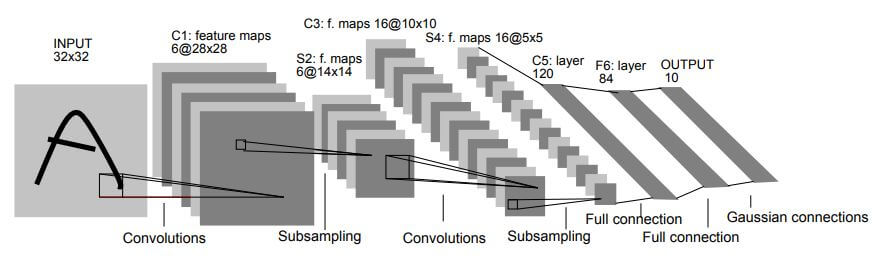
\includegraphics[width=0.8\linewidth]{reports//assets/lenet.jpg}
    \caption[LeNet CNN]{LeNet, considerada la primera arquitectura CNN para el reconocimiento de dígitos \cite{lecun_gradient-based_1998}.}
    \label{fig:lenet}
\end{figure}

\subsection{Componentes principales}

\textbf{Capas convolucionales}

Una capa convolucional es una parte fundamental de una CNN que escanea la imagen de entrada con pequeños filtros (kernels), realizando una operación de convolución, que consiste en un producto punto deslizante entre el filtro y regiones locales de la imagen. Este proceso crea mapas de características que resaltan patrones importantes, como bordes o texturas \cite{noauthor_what_2021}. Estos mapas de características se transfieren a capas adicionales para extraer características más complejas. La Figura \ref{fig:convolution_feature_map} ilustra la operación de convolución y un ejemplo de mapa de características de una imagen mamaria.

\begin{figure}[h!]
	\centering
	\begin{subfigure}[c]{0.45\textwidth}
		\centering
		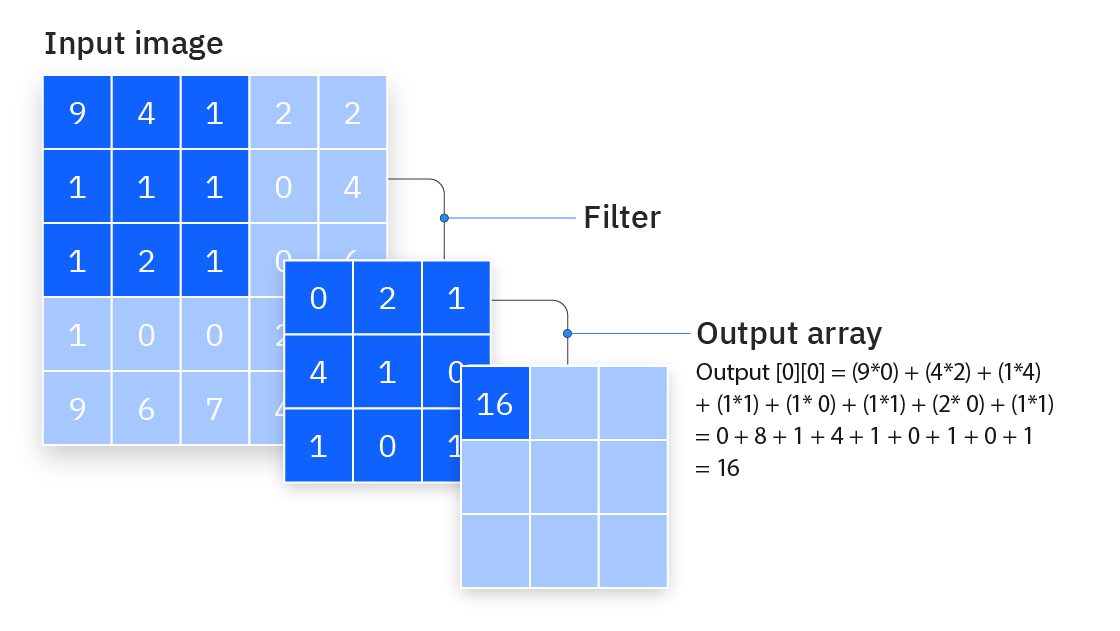
\includegraphics[width=\textwidth]{reports/assets/convolution.png}
            \caption{}
		\label{fig:convolution}
	\end{subfigure}
	\begin{subfigure}[c]{0.25\textwidth}
		\centering
		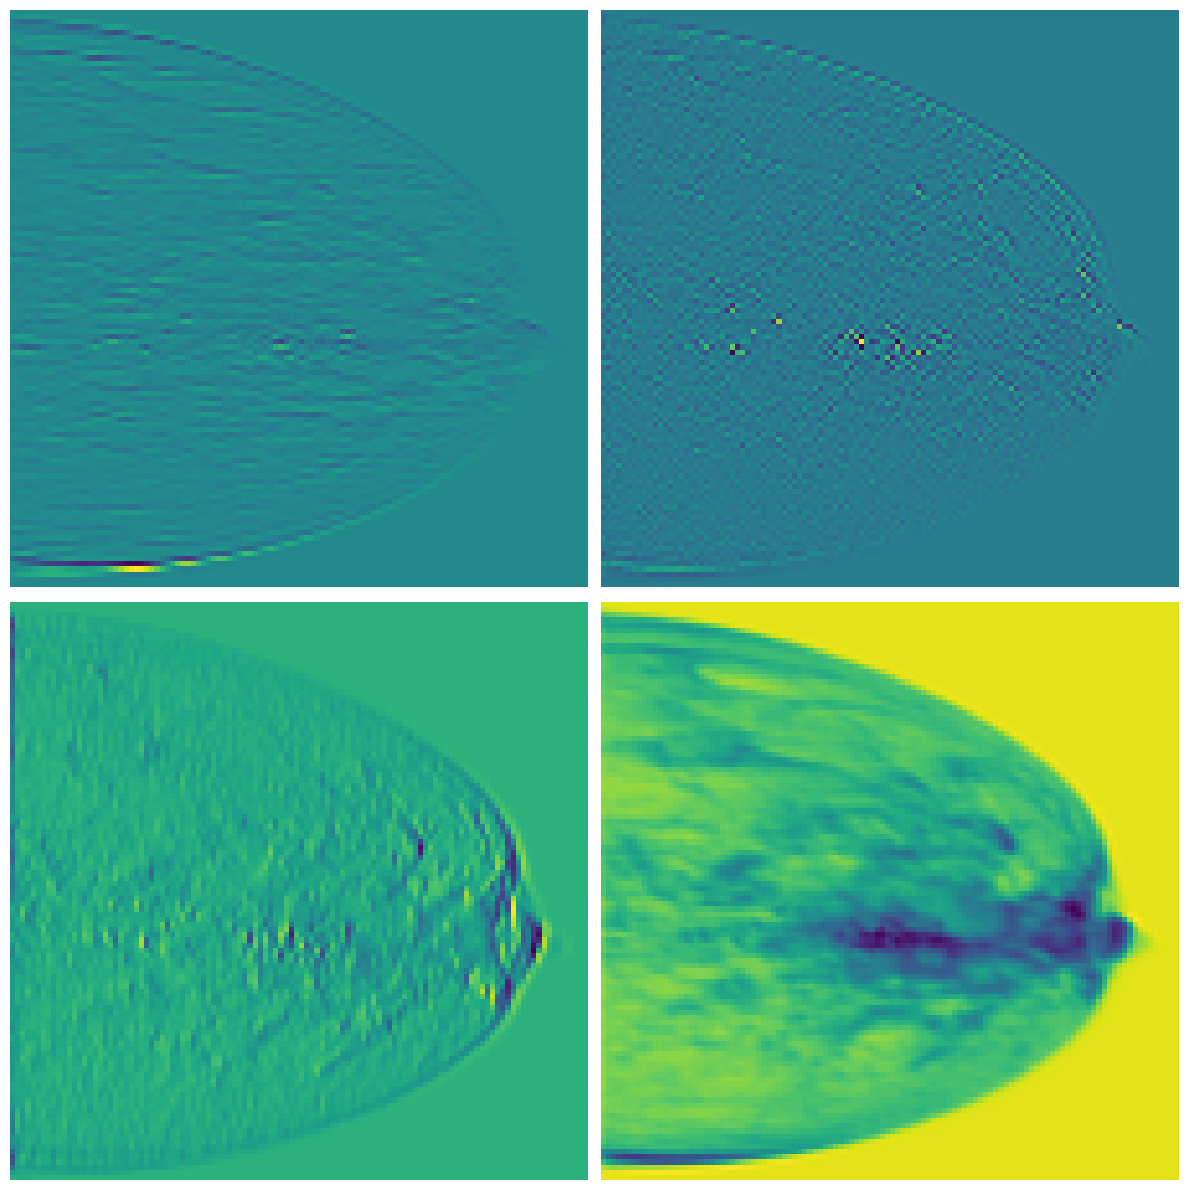
\includegraphics[width=\textwidth]{reports/assets/feature_maps_resnet.png}
            \caption{}
		\label{fig:feature_map_conv}
	\end{subfigure}
	\caption[Convolución y mapa de características]{(a) Ilustración de la operación de convolución \cite{noauthor_what_2021}. (b) Mapas de características mamarias extraídos de la primera capa convolucional de Resnet101.}
\label{fig:convolution_feature_map}
\end{figure}

\textbf{Funciones de activación}

Las funciones de activación introducen no linealidad en las redes neuronales, permitiendo que aprendan patrones complejos y no solo relaciones lineales \cite{langActivationFunctionsNeural2024}. Normalmente, se aplican tras las operaciones de convolución para producir los mapas de características. Entre las distintas funciones de activación, la unidad lineal rectificada (ReLU) es la más utilizada en las CNN por su simplicidad, eficiencia computacional y su capacidad para abordar el problema del gradiente desvanecido\footnote{La dificultad de entrenar redes profundas causada por gradientes que se vuelven muy pequeños al propagarse por muchas capas.}. Las funciones de activación más populares se muestran en la Figura \ref{fig:activations-functions}.

\begin{figure}
    \centering
    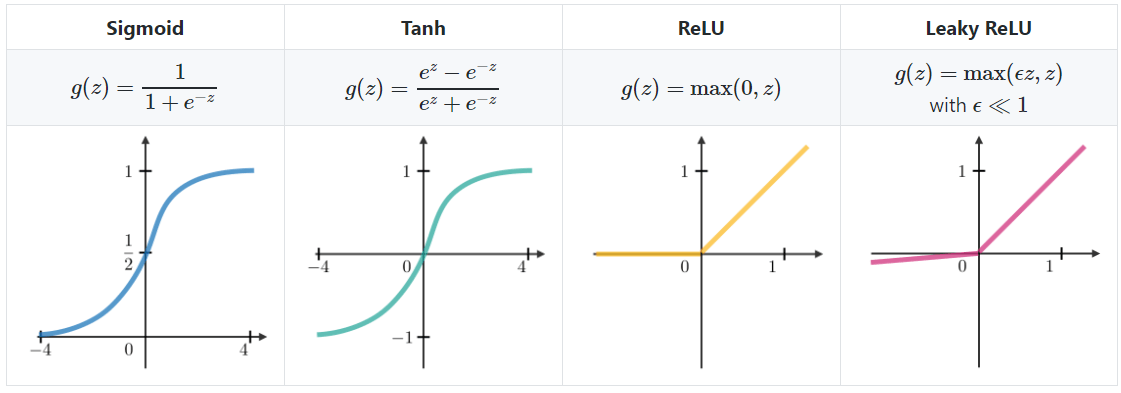
\includegraphics[width=1.0\linewidth]{reports//assets/activations_functions.png}
    \caption[Funciones de activación populares]{Funciones de activación populares usadas en CNN \cite{wachtelUnderstandingActivationFunctions2021}.}
    \label{fig:activations-functions}
\end{figure}

\textbf{Capas de pooling (agrupamiento)}

Las capas de pooling reducen las dimensiones espaciales de los mapas de características, disminuyendo la complejidad computacional y ayudando a controlar el sobreajuste\footnote{Un problema común en el aprendizaje automático donde un modelo aprende demasiado los datos de entrenamiento, en lugar de captar patrones que generalicen a datos nuevos y no vistos.} \cite{brownlee_gentle_2019}. A diferencia de las capas convolucionales, las capas de pooling realizan operaciones de agrupamiento en lugar de convoluciones. Las operaciones más comunes son el max pooling, que selecciona el valor máximo de una región, y el average pooling, que calcula el valor medio de una región (Figura \ref{fig:pooling_operations}). El pooling suele aplicarse tras las funciones de activación y se repite a lo largo de la red.

\begin{figure}[h!]
    \centering
    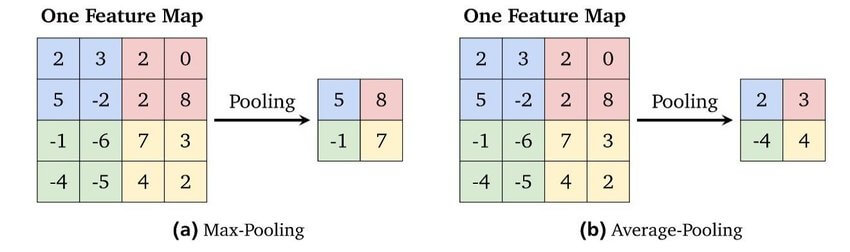
\includegraphics[width=1.0\linewidth]{reports//assets/pooling.jpg}
    \caption[Operaciones de pooling populares]{Representación de max pooling y average pooling \cite{SkinLesionClassification}.}
    \label{fig:pooling_operations}
\end{figure}

\textbf{Capa totalmente conectada}

Las capas totalmente conectadas, o densas, suelen situarse cerca del final de una red neuronal convolucional (CNN). Conectan cada neurona de la capa anterior, consolidando las características extraídas por las capas convolucionales y de pooling en una representación global. Los mapas de características se aplanan en un vector unidimensional antes de entrar en estas capas, facilitando el mapeo de las características extraídas a salidas como probabilidades de clase \cite{noauthor_fully_nodate}. La Figura \ref{fig:fc_layers} ilustra una red neuronal con varias capas totalmente conectadas.

\begin{figure}[h!]
    \centering
    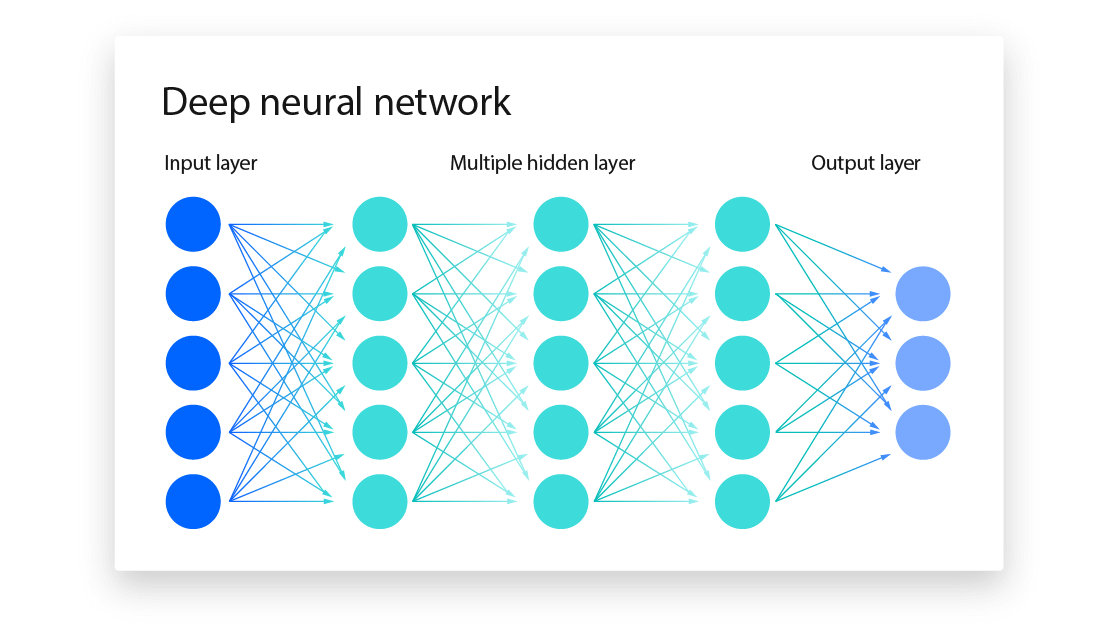
\includegraphics[width=0.75\linewidth]{reports//assets/fc_network.png}
    \caption[Capas totalmente conectadas]{Red neuronal con tres capas totalmente conectadas y tres salidas \cite{bergmann_what_2024}.}
    \label{fig:fc_layers}
\end{figure}


\textbf{Entrenamiento}

Con todos estos bloques de construcción, se construyen las CNN. Una vez que se define una red, esta pasa por el proceso de entrenamiento, que implica los siguientes pasos \cite{bergmann_what_2024}:

\begin{enumerate}
\item \textbf{Propagación hacia adelante}: Los datos de entrada pasan a través de la red, capa por capa, para producir una predicción de salida.
\item \textbf{Cálculo de la función de pérdida}: La diferencia entre la salida predicha y la etiqueta verdadera se mide utilizando una función de pérdida.
\item \textbf{Retropropagación}: La red calcula los gradientes de la pérdida con respecto a cada parámetro, propagando el error hacia atrás a través de las capas.
\item \textbf{Descenso del gradiente}: La red actualiza sus parámetros (pesos y sesgos) utilizando los gradientes calculados para minimizar la pérdida.
\end{enumerate}

Después del entrenamiento, la red está lista para hacer predicciones sobre datos nuevos y no vistos. La Figura \ref{fig:cnn_breast} muestra un ejemplo de una arquitectura CNN completa para la predicción de cáncer de mama.

\begin{figure}[h!]
\centering
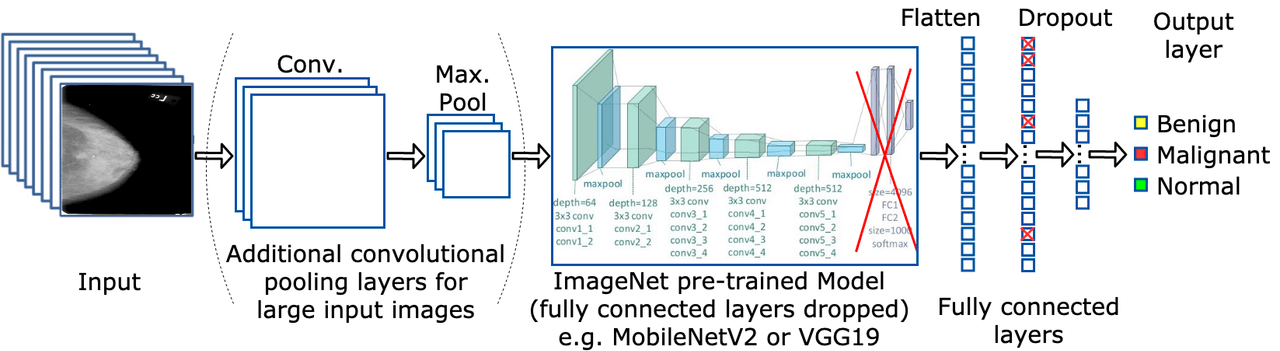
\includegraphics[width=0.9\linewidth]{reports//assets/cnn_breast.png}
\caption[Breast cancer CNN]{CNN para la predicción de cáncer de mama \cite{jaamour_divide_2023}.}
\label{fig:cnn_breast}
\end{figure}

\subsection{Principales Arquitecturas}

\textbf{VGGNet (VGG16/VGG19)}

Symonyan et al. (2015) introdujeron las VGGNets \cite{simonyanVeryDeepConvolutional}. Reconocidas por su diseño sencillo y profundidad, emplean únicamente convoluciones de 3×3 y pueden tener hasta 19 capas. Se utilizan ampliamente como extractores de características y sirven como referencia fundamental para el aprendizaje por transferencia tanto en aplicaciones médicas como de imágenes generales.

\textbf{ResNet}

He et al. (2015) \cite{he_deep_2015} presentaron las Redes Residuales, o ResNets, como una solución para entrenar redes neuronales muy profundas con más de 50 capas, lo que ayuda a abordar el problema de los gradientes que desaparecen. Esto se logra mediante la implementación de conexiones residuales o de salto entre capas. ResNet es la opción predeterminada para muchas tareas de análisis de imágenes debido a su robustez y facilidad de entrenamiento.

Como se indicó anteriormente, este estudio utiliza ResNet-101 como modelo base. Esta arquitectura, compuesta por 101 capas con conexiones residuales, resulta altamente eficiente para gestionar tareas complejas. La Figura \ref{fig:resnet_101} ilustra una visión general de su estructura.

\begin{figure}[h!]
\centering
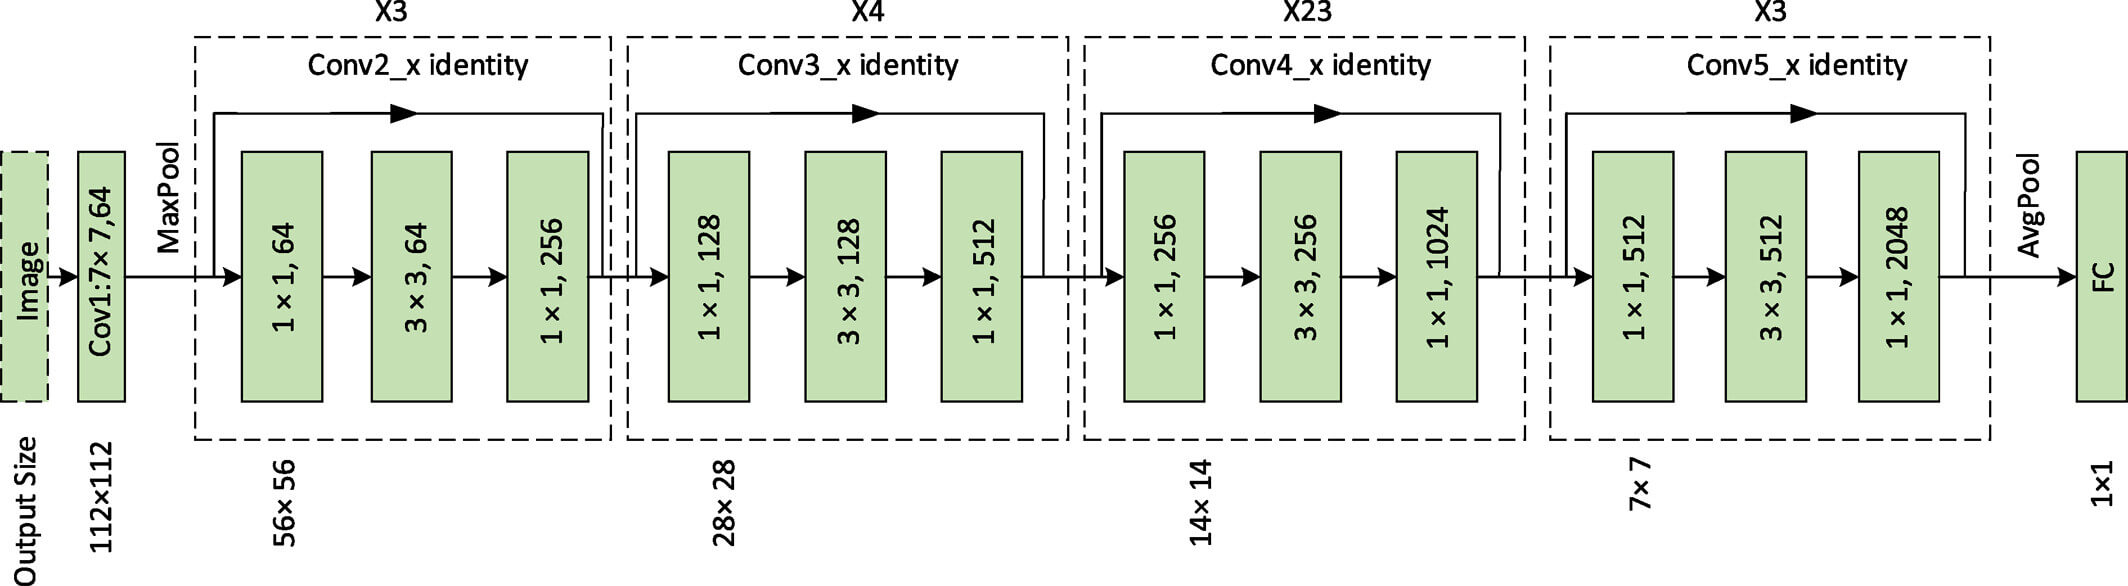
\includegraphics[width=0.75\linewidth]{reports//assets/resnet101.jpg}
\caption[ResNet-101 Architecture]{Arquitectura de ResNet-101.}
\label{fig:resnet_101}
\end{figure}

\subsection{Limitaciones de las CNN}

Las CNN ofrecen numerosas ventajas y una amplia gama de aplicaciones; sin embargo, también presentan ciertas limitaciones que merecen consideración:


\begin{itemize}
\item \textbf{Contexto global limitado}: Las CNN capturan principalmente características locales y tienen dificultades con el contexto global, que es importante en la imagen médica.
\item \textbf{Sesgo inductivo rígido}: Su diseño impone suposiciones como la localidad y la invariancia a la traslación, lo que limita la flexibilidad para aprender patrones más abstractos o no locales.

\item \textbf{Generalización en datos diversos}: Las CNN a menudo tienen dificultades para generalizar a datos de diferentes fuentes o poblaciones de pacientes, reduciendo su robustez en entornos clínicos.
\end{itemize}

Los avances recientes en modelos basados en Transformers ofrecen soluciones prometedoras a algunas de estas limitaciones al permitir un mejor modelado del contexto global y mejorar la generalización, lo que se discutirá en la siguiente sección.

\section{Modelos basados en Transformers}

Los modelos Transformer se construyen sobre la arquitectura Transformer, que fue desarrollada inicialmente para tareas de procesamiento de lenguaje natural (NLP). Desde su introducción en la visión por computadora, estos modelos han ganado una popularidad significativa como alternativa a las CNN debido a su eficacia para capturar el contexto global y modelar dependencias de largo alcance dentro de las imágenes \cite{pereira_review_2024}.

En esta sección, revisamos qué son los modelos basados en Transformers y describimos los diseños arquitectónicos de aquellos analizados en este trabajo para la tarea de clasificación de subtipos moleculares de cáncer de mama.

\subsection{La arquitectura Transformer}

La arquitectura Transformer es un modelo de aprendizaje profundo presentado por Vaswani et al. (2017) en su artículo seminal “Attention is All You Need” \cite{vaswani_attention_2017}. Originalmente desarrollada como una alternativa a las redes neuronales recurrentes (RNN)\footnote{Una clase especial de red neuronal artificial diseñada para procesar datos secuenciales o series temporales, como texto, voz o lecturas de sensores.} para tareas de secuencia a secuencia en NLP, el Transformer ha sido ampliamente adoptado también en visión por computadora.

En su núcleo, el Transformer consiste en una estructura codificador-decodificador construida a partir de capas repetidas que contienen dos componentes clave: la auto-atención multi-cabeza y las redes feed-forward por posición (ver Figura~\ref{fig:transformer}). Este diseño permite que el modelo capture dependencias tanto locales como globales al relacionar cada elemento de la secuencia de entrada con todos los demás elementos, independientemente de sus posiciones.

\begin{figure}[h!]
    \centering
    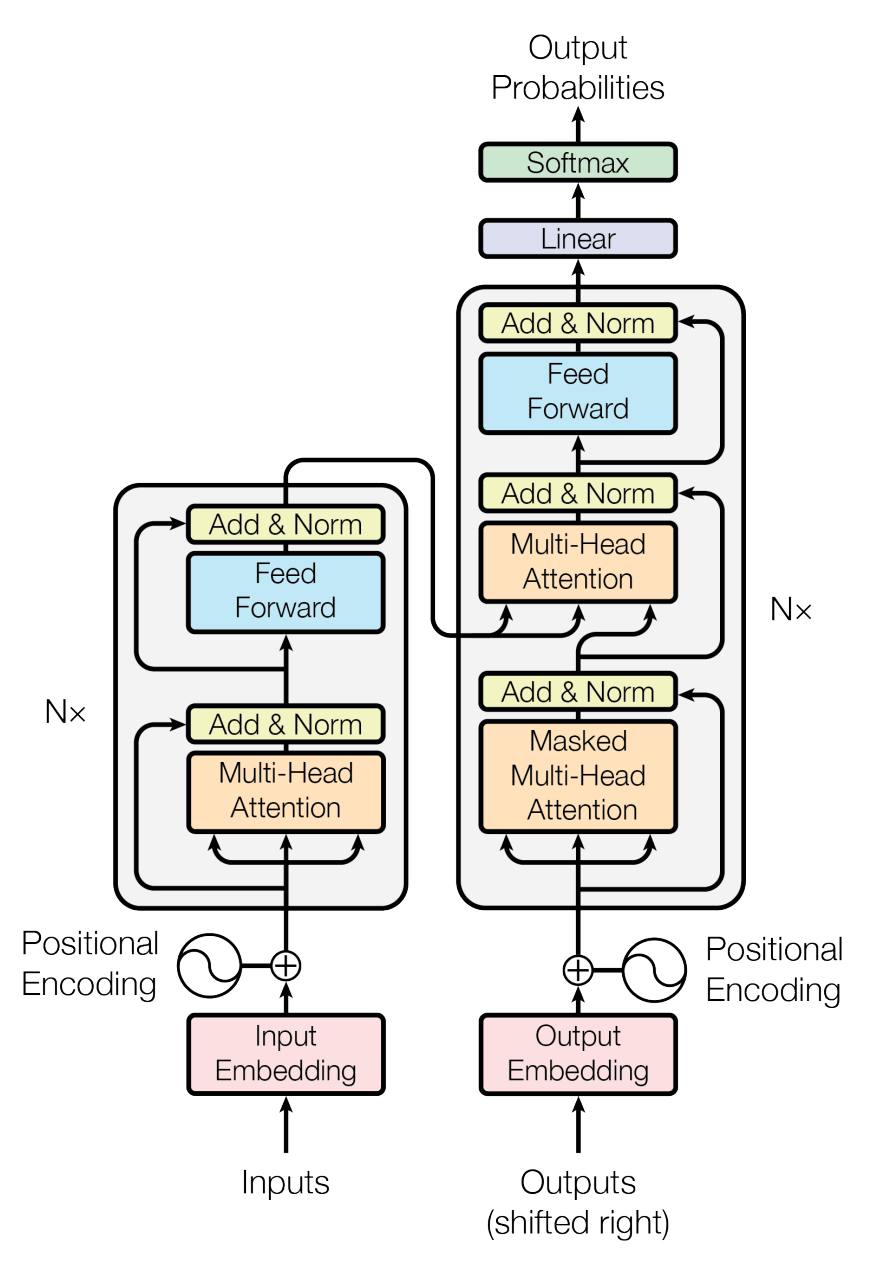
\includegraphics[width=0.5\linewidth]{reports//assets/transformer.png}
    \caption[Transformer Architecture]{The Transformer Architecture \cite{vaswani_attention_2017}.}
    \label{fig:transformer}
\end{figure}

\textbf{Auto-atención}

La auto-atención es un mecanismo de atención\footnote{Una técnica en aprendizaje automático que permite a los modelos centrarse en las partes más relevantes de los datos de entrada al hacer predicciones o generar salidas.} que permite a una red relacionar diferentes posiciones dentro de una misma secuencia de entrada, calculando así una representación consciente del contexto para cada elemento. En términos más simples, permite que el modelo priorice e integre de manera eficiente la información importante de toda la entrada. El concepto de atención fue introducido por primera vez por Bahdanau et al. (2014) \cite{bahdanau_neural_2014}, pero fue la arquitectura Transformer la que primero dependió completamente de la auto-atención para calcular representaciones \cite{vaswani_attention_2017}. De manera concisa, este proceso funciona de la siguiente manera:

\begin{itemize}
\item \textbf{Proyección}: Cada elemento de entrada se proyecta en tres vectores distintos:
\begin{itemize}
\item \textbf{Query (Q)}: Representa el elemento actual (por ejemplo, una palabra o un parche de imagen) para el cual queremos encontrar información relevante en la secuencia.
\item \textbf{Key (K)}: Representa cada elemento de la secuencia y se utiliza para comparar con las queries y medir su relevancia.
\item \textbf{Value (V)}: Contiene la información real de cada elemento, que se combinará según los puntajes de atención.
\end{itemize}
\item \textbf{Cálculo de puntuaciones}: Para cada elemento, se calcula un puntaje de atención tomando el producto punto entre su query y todas las keys de la secuencia.
\item \textbf{Escalado}: Cada puntaje se divide por la raíz cuadrada de la dimensión de las keys para estabilizar el entrenamiento y evitar gradientes grandes.
\item \textbf{Normalización Softmax}: La función softmax\footnote{La función softmax transforma los puntajes en probabilidades que suman uno.} se aplica a los puntajes escalados para obtener los pesos de atención.
\item \textbf{Suma ponderada}: Se obtiene una nueva representación, consciente del contexto, para cada elemento de entrada calculando la suma ponderada de todos los vectores value utilizando los pesos de atención.
\end{itemize}

La Figura \ref{fig:scaled_dot_product_attn} ilustra en detalle el proceso de atención de producto punto escalado. Matemáticamente, el proceso puede resumirse de la siguiente manera:

$$Attention(Q,K,V) = softmax\left(\frac{QK^T}{\sqrt{d_k}}\right)V$$

\begin{figure}[h!]
\centering
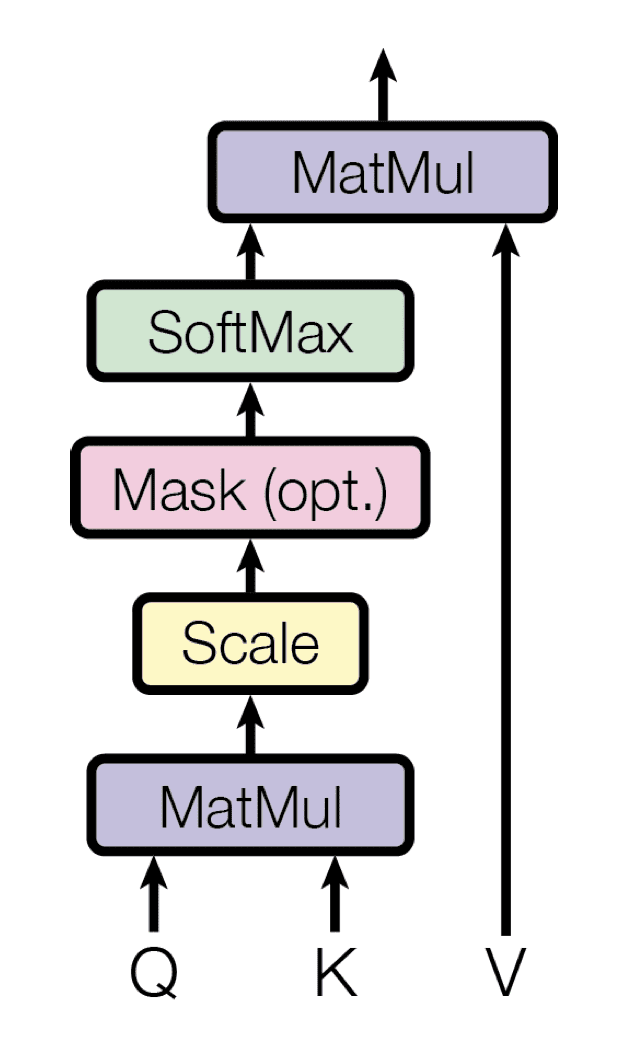
\includegraphics[width=0.3\linewidth]{reports//assets/scaled_dot_product.png}
\caption[Scaled dot-product attention]{Mecanismo de atención de producto punto escalado \cite{vaswani_attention_2017}.}
\label{fig:scaled_dot_product_attn}
\end{figure}


\subsection{Vision Transformer}

Un Vision Transformer (ViT) es una arquitectura de aprendizaje profundo introducida por Dosovitskiy et al. (2020) \cite{dosovitskiy_image_2020} diseñada para tareas de visión por computadora, inspirada en la arquitectura Transformer desarrollada originalmente para NLP.

\textbf{Flujo de procesamiento de ViT}

Un ViT procesa una imagen dividiéndola primero en parches de tamaño fijo; por ejemplo, una imagen de 224×224 dividida en parches de 16×16 resulta en 196 parches. Cada parche se aplana y se proyecta a un espacio de embedding mediante la capa de embedding de parches. Dado que la arquitectura ViT carece de conciencia espacial inherente, se agregan codificaciones posicionales a cada embedding de parche para preservar la información espacial dentro de la imagen. Este diseño permite que la entrada se trate de manera análoga a una secuencia de tokens en los Transformers de NLP. A medida que la secuencia pasa por múltiples capas de auto-atención multi-cabeza, el modelo aprende a capturar relaciones tanto locales como globales entre los parches, permitiendo una comprensión robusta de la imagen. Este proceso y la arquitectura ViT se ilustran en la Figura \ref{fig:vit_arch}.

\begin{figure}[h!]
\centering
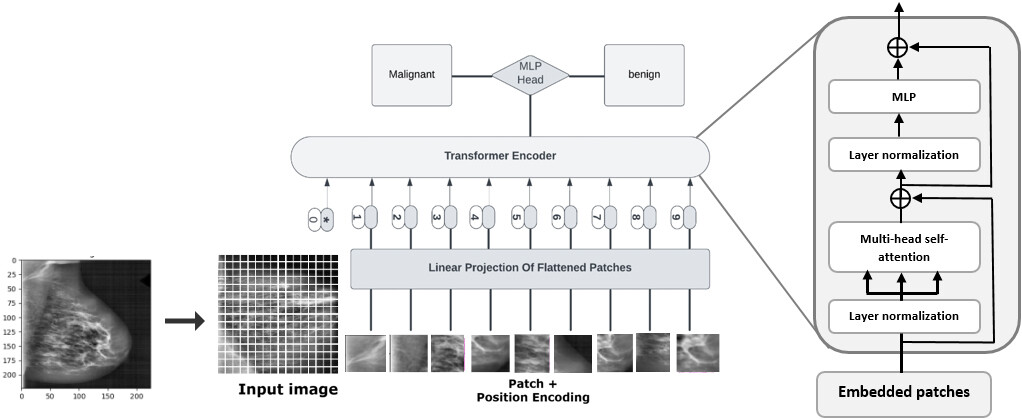
\includegraphics[width=1.0\linewidth]{reports//assets/vit_breast.jpg}
\caption[Vision Transformer Architecture]{Arquitectura ViT, en este ejemplo, para la clasificación de cáncer de mama \cite{abimouloud_vision_2024}.}
\label{fig:vit_arch}
\end{figure}

Los ViT han expandido rápidamente su alcance a muchas tareas de visión por computadora, incluyendo clasificación de imágenes, detección de objetos y segmentación de imágenes. En imagen médica, varios estudios han evaluado su rendimiento en tareas como la clasificación de cáncer de mama, reportando consistentemente resultados sólidos \cite{marquez_vara_vision_2024, mauricio_comparing_2023, ayana_vision-transformer-based_2023}.


\subsection{Shifted-Window Transformer}

Los Shifted-Window Transformers (Swin), introducidos por Liu et al. (2021) \cite{liu_swin_2021}, son una arquitectura especializada derivada de los Vision Transformers (ViT). Están diseñados para abordar algunas de las limitaciones de ViT, en particular en lo que respecta a la eficiencia computacional y la escalabilidad al procesar imágenes de alta resolución.

Para lograr esto, Swin emplea un mecanismo de ventanas desplazadas. A diferencia de ViT, que normalmente aplica la auto-atención de manera global, Swin divide la imagen en un conjunto de ventanas no superpuestas (Figura \ref{fig:swin_vit}), donde cada ventana contiene un subconjunto de parches de la imagen. La auto-atención se aplica localmente dentro de cada ventana, reduciendo significativamente la complejidad computacional. Las ventanas se desplazan entre capas para permitir conexiones entre ventanas y mejorar el flujo de información a lo largo de toda la imagen.

\begin{figure}[h!]
\centering
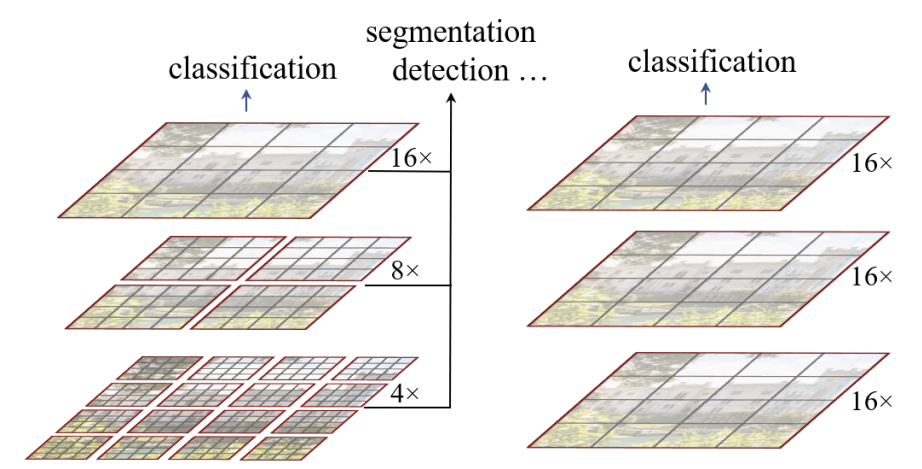
\includegraphics[width=0.6\linewidth]{reports//assets/Swin.png}
\caption[Comparison of Swin and ViT mechanisms]{Comparación de los mecanismos de atención de Swin y ViT. \textbf{Izquierda:} Swin Transformer con auto-atención en ventanas desplazadas. \textbf{Derecha:} Vision Transformer (ViT) con auto-atención global entre todos los parches \cite{liu_swin_2021}.}
\label{fig:swin_vit}
\end{figure}

Como resultado de este mecanismo, Swin exhibe una complejidad computacional de $O(n)$, mientras que ViT tiene una complejidad de $O(N^2)$.


\begin{figure}[h!]
\centering
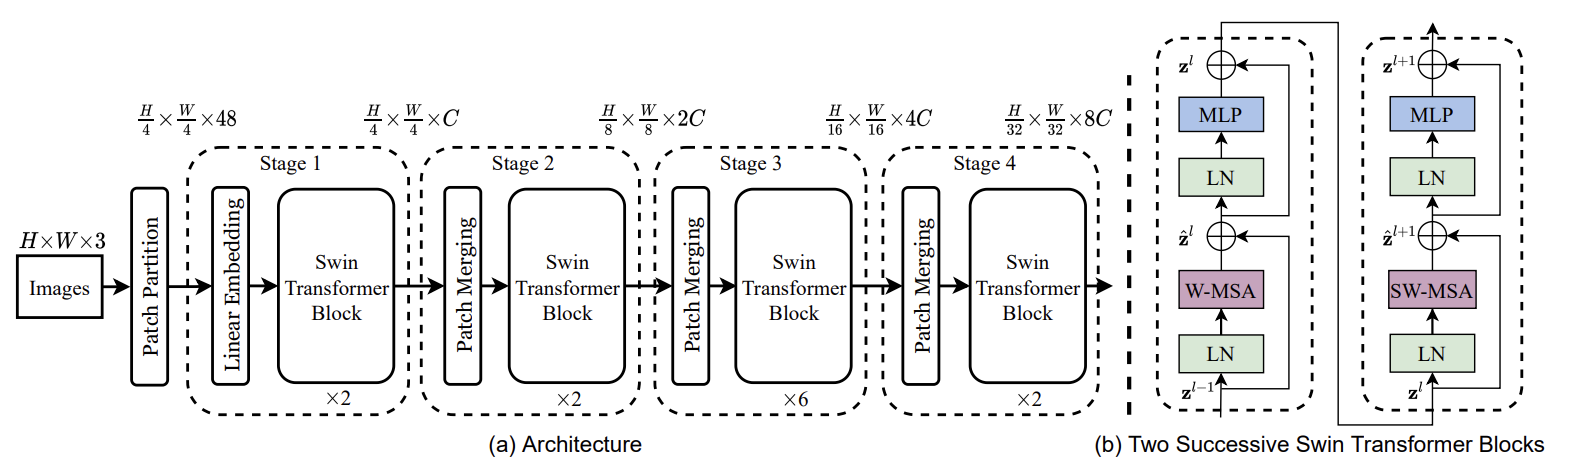
\includegraphics[width=1.0\linewidth]{reports//assets/SwinArch.png}
\caption[Swin Transformer Arch]{Arquitectura Swin Transformer \cite{liu_swin_2021}.}
\label{fig:swin_arch}
\end{figure}

\subsection{Multi-Axis Vision Transformer}

Multi-Axis Vision Transformer (MaxViT) es una arquitectura híbrida de vision transformer introducida por Tu et al. (2022) \cite{tu_maxvit_2022}. Está diseñada para capturar tanto relaciones espaciales locales como globales en imágenes, superando las limitaciones de escalabilidad y capacidad de modelos previos basados en transformers. MaxViT logra esto combinando atención local en bloques (como en Swin, pero sin desplazamiento) y atención global dilatada (en cuadrícula) dentro de cada bloque, junto con capas convolucionales. Este mecanismo de atención multi-eje permite que MaxViT modele eficientemente dependencias tanto de corto como de largo alcance, manteniendo la misma complejidad computacional lineal que Swin. La Figura \ref{fig:max_vit_arch} ilustra esta estructura.

\begin{figure}[h!]
\centering
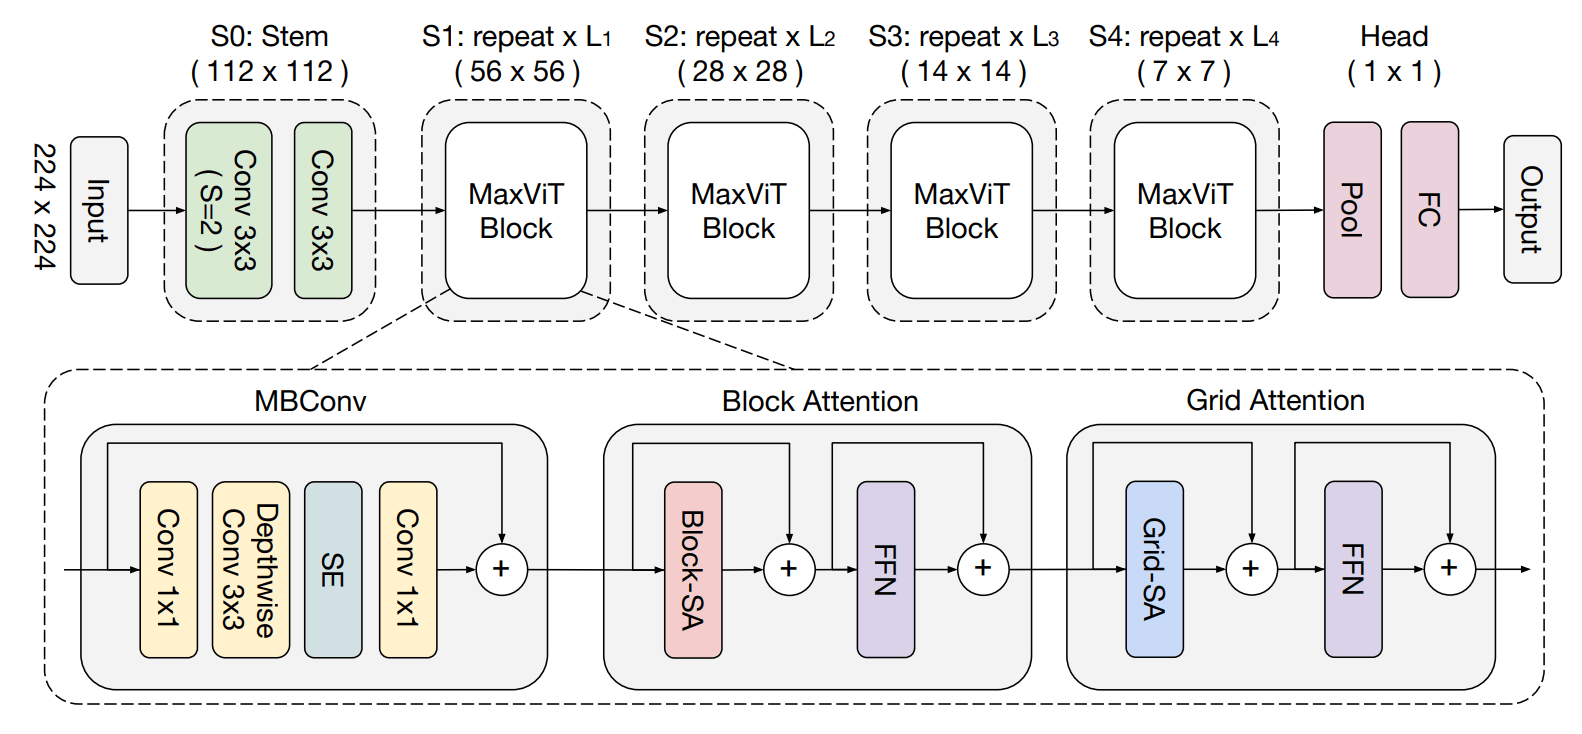
\includegraphics[width=1.0\linewidth]{reports//assets/maxvit_arch.png}
\caption[Multi-Axis Vision Transformer Arch]{Arquitectura MaxVit \cite{tu_maxvit_2022}.}
\label{fig:max_vit_arch}
\end{figure}

\textbf{Atención Multi-Eje}

La atención multi-eje es el componente clave de MaxViT. Funciona dividiendo el mecanismo de atención en dos partes: un bloque de atención local, que se enfoca en regiones locales (similar al de Swin), y un bloque de atención en cuadrícula, que permite el flujo de información global a través de toda la imagen mediante un patrón dilatado en cuadrícula. Este diseño permite que MaxViT capture eficientemente dependencias tanto locales como globales dentro de cada bloque (ver Figura \ref{fig:multi_axis_attention}).

\begin{figure}[h!]
\centering
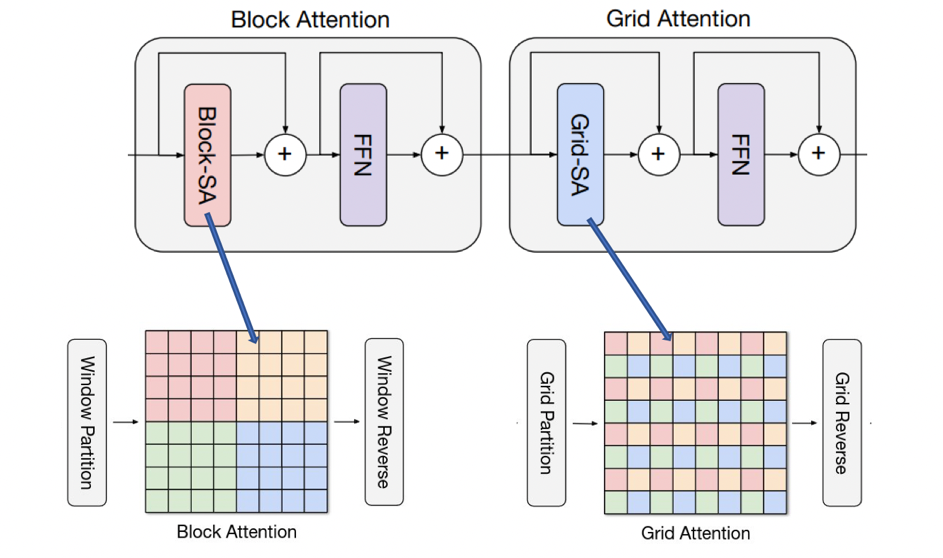
\includegraphics[width=0.6\linewidth]{reports//assets/multi_axis_attention.png}
\caption[Multi-Axis Attention Blocks]{Bloques de atención multi-eje \cite{noauthor_maxvit-unet_2024}.}
\label{fig:multi_axis_attention}
\end{figure}

\section{Técnicas de Entrenamiento y Evaluación}

\subsection{Transferencia de Aprendizaje}

La transferencia de aprendizaje es una técnica de aprendizaje automático en la que un modelo desarrollado y entrenado en una tarea o conjunto de datos se reutiliza o ajusta para mejorar el rendimiento en una tarea diferente, pero relacionada. Es especialmente valiosa cuando los datos son limitados o la tarea objetivo dispone de pocos ejemplos etiquetados \cite{murel_what_2024}. En otras palabras, en lugar de entrenar un modelo nuevo desde cero, la transferencia de aprendizaje aprovecha el conocimiento previamente obtenido, como características y pesos aprendidos, a menudo de grandes conjuntos de datos, para acelerar y mejorar el aprendizaje en un nuevo problema.

Este enfoque es muy popular y ampliamente utilizado para evitar entrenar modelos de aprendizaje automático o profundo desde cero. En imagen médica, por ejemplo, donde los datos anotados suelen ser escasos o costosos de obtener, la transferencia de aprendizaje ha permitido el desarrollo y entrenamiento de modelos que reducen el tiempo de entrenamiento, mejoran el rendimiento y promueven la reutilización de características \cite{matsoukas_what_2022}. Este proceso se muestra en la Figura \ref{fig:transfer_learning}.

\begin{figure}[h!]
\centering
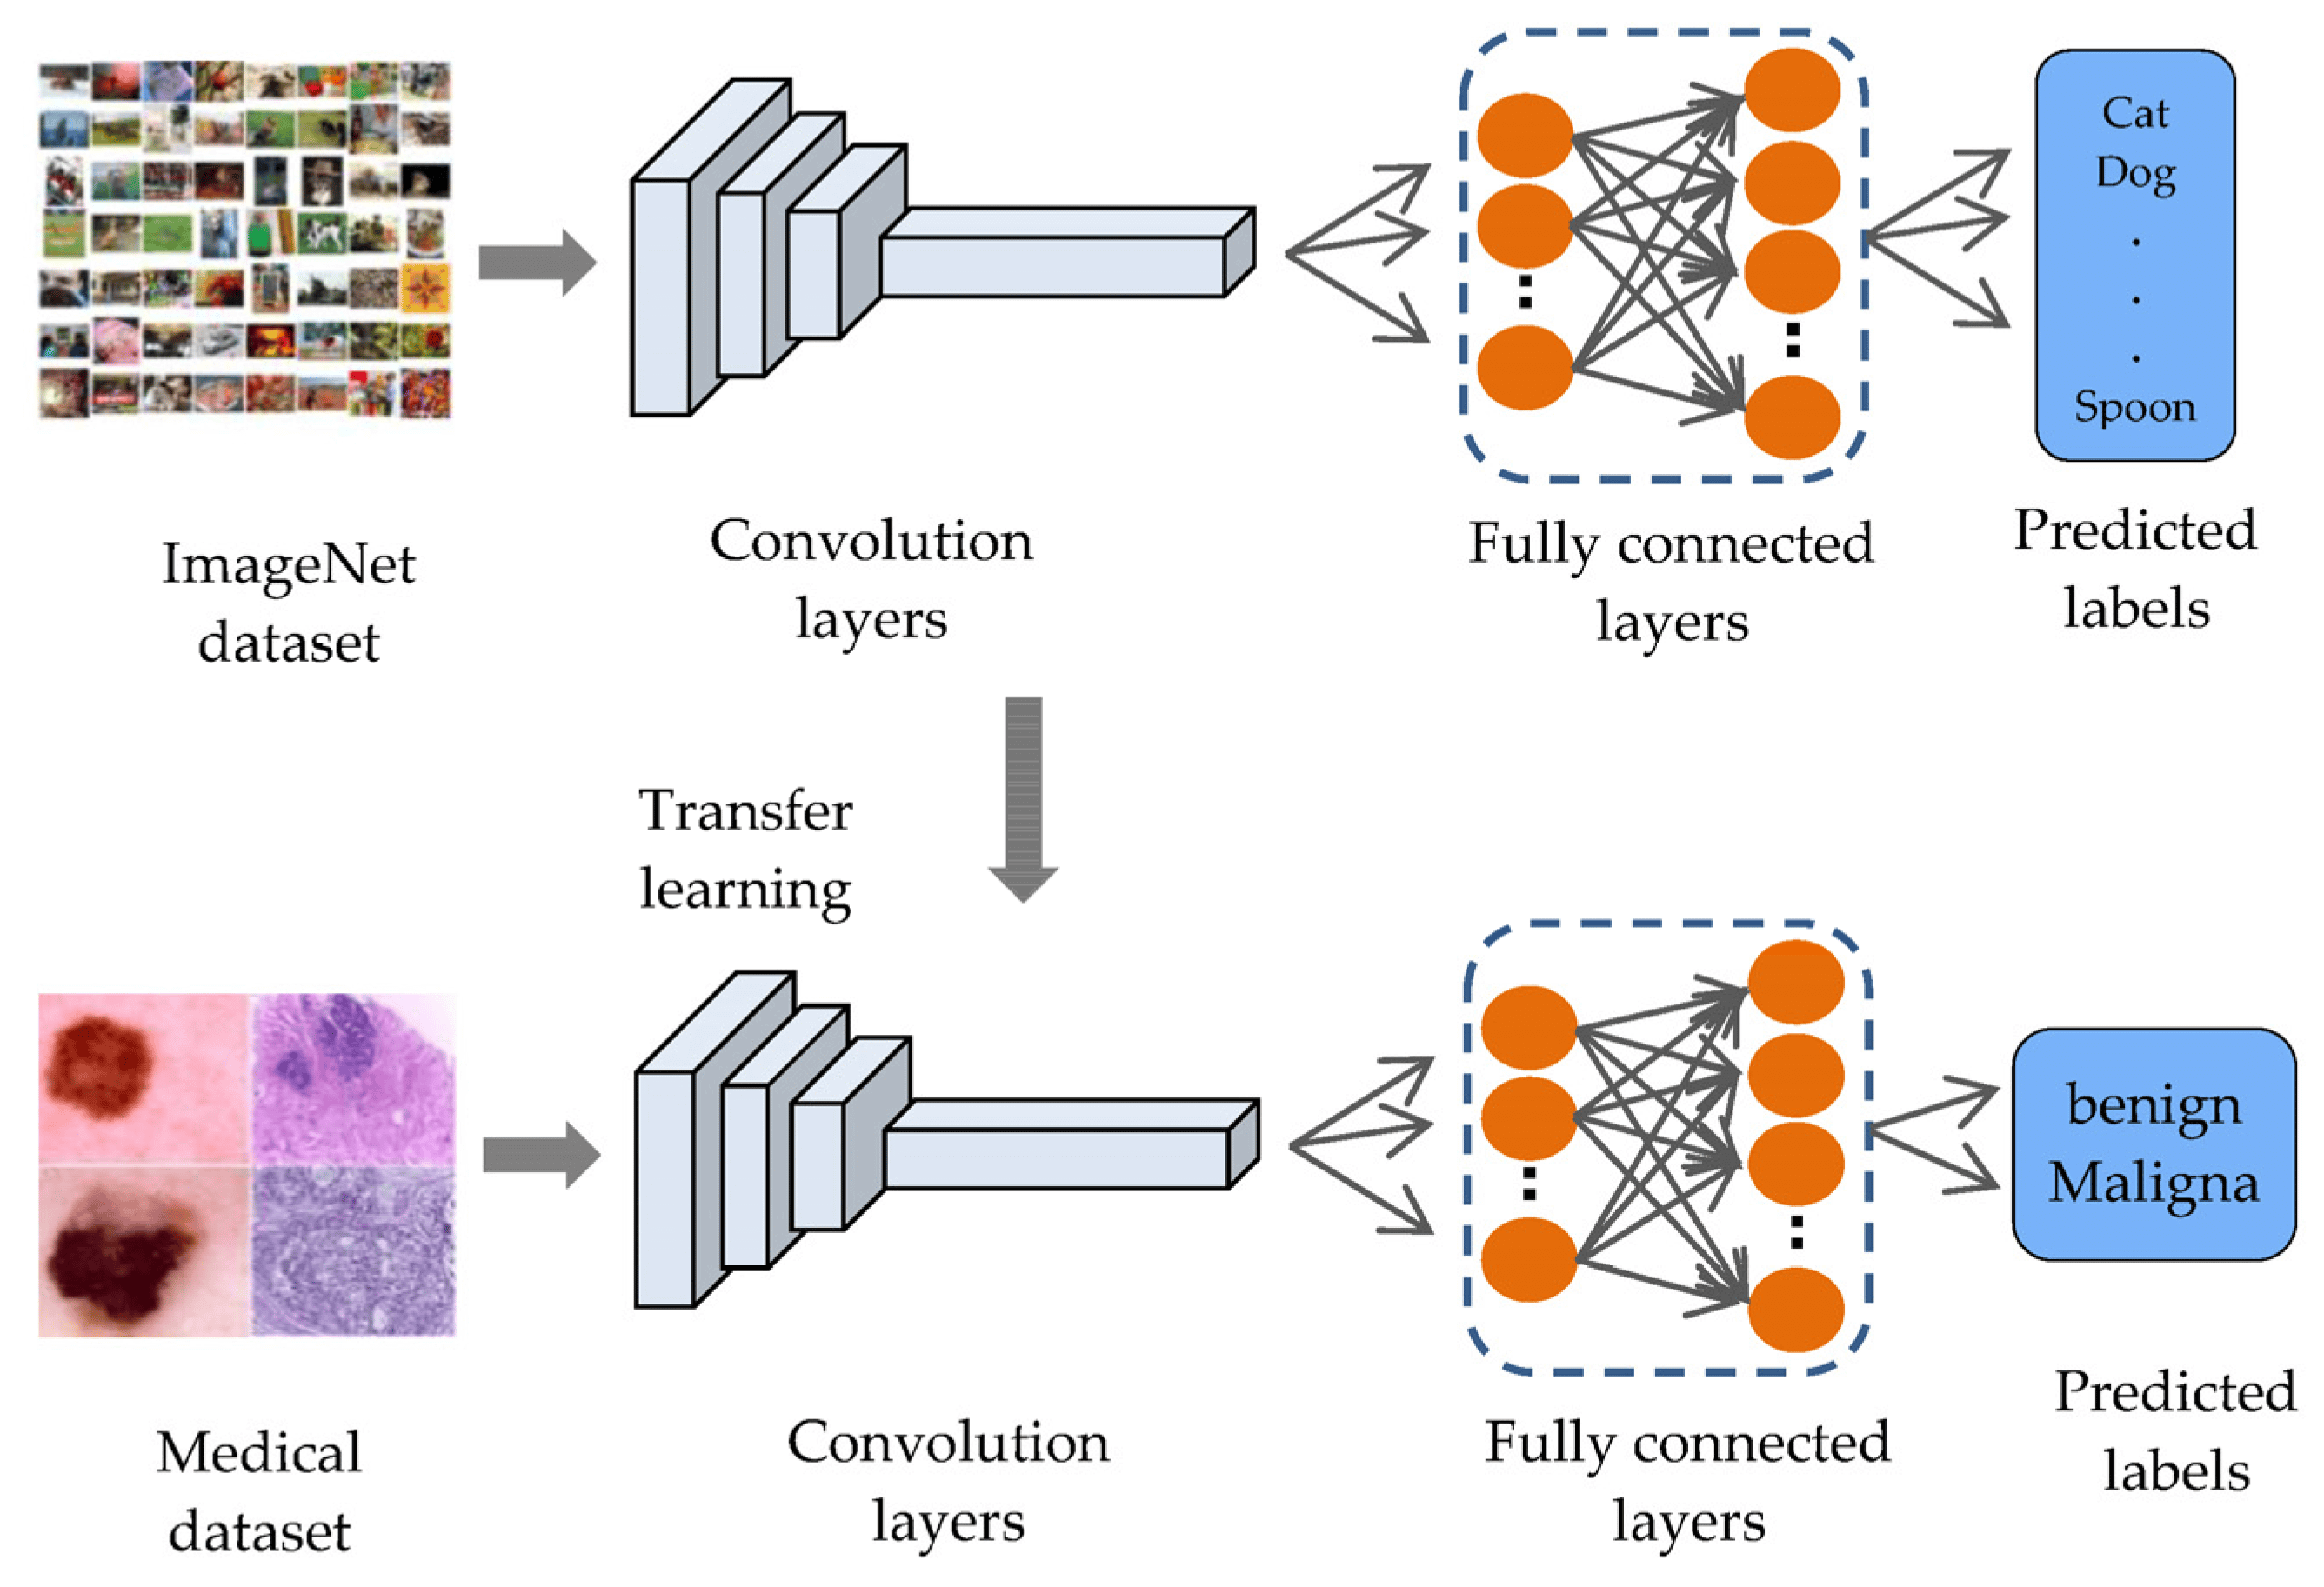
\includegraphics[width=0.75\linewidth]{reports//assets/transfer-learning.png}
\caption[Transfer learning process]{Proceso de transferencia de aprendizaje donde}
\label{fig:transfer_learning}
\end{figure}

\subsection{Ajuste Fino (Fine-Tuning)}

El ajuste fino es una técnica específica dentro de la transferencia de aprendizaje que consiste en tomar un modelo preentrenado y continuar su entrenamiento en un conjunto de datos más pequeño o especializado para adaptar sus capacidades a un caso o dominio particular \cite{noauthor_what_2024}. Durante el ajuste fino, algunos o todos los parámetros del modelo se descongelan y actualizan, permitiendo que el modelo aprenda características relevantes para la nueva tarea mientras retiene el conocimiento general adquirido durante el preentrenamiento. Sin embargo, entrenar modelos grandes en conjuntos de datos pequeños puede llevar a sobreajuste, por lo que es común utilizar una tasa de aprendizaje más baja durante el ajuste fino para realizar ajustes graduales y preservar las representaciones previamente aprendidas.

\subsection{Validación Cruzada K-Fold}

La validación cruzada K-Fold es una técnica de evaluación robusta utilizada en aprendizaje automático cuando los datos son limitados o una sola partición de entrenamiento/prueba puede no proporcionar resultados fiables. El conjunto de datos se divide en $K$ partes iguales, o folds. El modelo se entrena y valida $K$ veces, utilizando cada vez un fold diferente como conjunto de validación y los folds restantes para entrenamiento. Este proceso asegura que cada muestra se utilice tanto para entrenamiento como para validación, lo que conduce a una estimación más fiable y menos sesgada del rendimiento del modelo. Al promediar los resultados de todos los folds, la validación cruzada K-Fold reduce la varianza y es especialmente útil para conjuntos de datos pequeños o desbalanceados. La Figura \ref{fig:k_fold} ilustra este proceso.

\begin{figure}[h!]
\centering
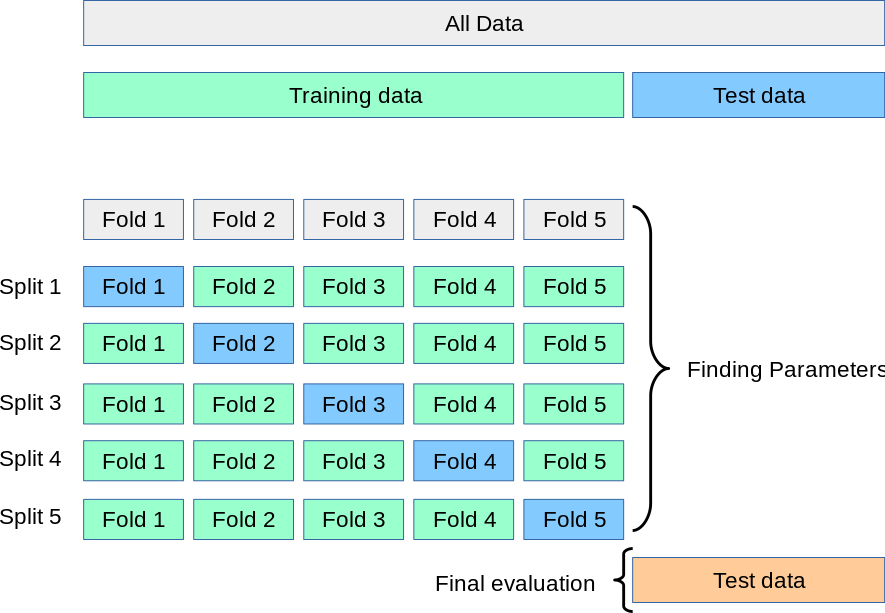
\includegraphics[width=0.75\linewidth]{reports//assets/k-fold.png}
\caption[K-Fold Cross Validation]{Proceso de validación cruzada K-Fold, en este ejemplo, $K$ = 5 \cite{noauthor_31_nodate}.}
\label{fig:k_fold}
\end{figure}

\subsection{Explicabilidad en IA}

Los modelos de aprendizaje profundo, aunque altamente efectivos en el análisis de imágenes médicas, suelen ser criticados por su falta de interpretabilidad, comúnmente conocida como el problema de la “caja negra”\footnote{Se refiere a un sistema cuyos mecanismos internos son opacos y no fácilmente comprensibles, incluso para sus creadores.}. Las técnicas de explicabilidad buscan abordar este desafío proporcionando información visual o cuantitativa sobre el proceso de toma de decisiones de estos modelos. En el contexto de la detección de cáncer de mama y la subtipificación molecular a partir de imágenes mamográficas, la transparencia del modelo es especialmente importante para generar confianza clínica y ayudar a los radiólogos a comprender las predicciones impulsadas por IA. Se presentan dos métodos de explicabilidad de última generación: Grad-CAM, diseñado para redes neuronales convolucionales, y ViT-ReciproCAM, adaptado para Vision Transformers.

\textbf{Grad-CAM}

Grad-CAM (Gradient-weighted Class Activation Mapping) es una técnica de explicabilidad para CNNs que crea explicaciones visuales resaltando las regiones clave en las imágenes de entrada que influyen significativamente en la predicción del modelo \cite{noauthor_161002391_nodate}. Calcula los gradientes de la puntuación de la clase objetivo respecto a los mapas de características de una capa convolucional seleccionada para generar un mapa de localización específico de la clase. Esta técnica ayuda a interpretar las regiones de la imagen que contribuyen a las decisiones del modelo, siendo especialmente útil en imagen médica donde la transparencia es crítica.

\textbf{ViT-ReciproCAM}

ViT-ReciproCAM es un método de explicabilidad reciente diseñado específicamente para Vision Transformers (ViTs). A diferencia de técnicas tradicionales como Grad-CAM, que dependen de información de gradientes y atención, ViT-ReciproCAM no utiliza gradientes ni atención \cite{byun_vit-reciprocam_2023}. Opera enmascarando tokens en el mapa de características del último bloque codificador del transformer y midiendo el efecto de estas máscaras en la salida del modelo. Este proceso explota la correlación entre los tokens enmascarados y las predicciones de la red para una clase dada, produciendo mapas de saliencia localizados que indican las regiones de imagen más influyentes.

\begin{figure}
\centering
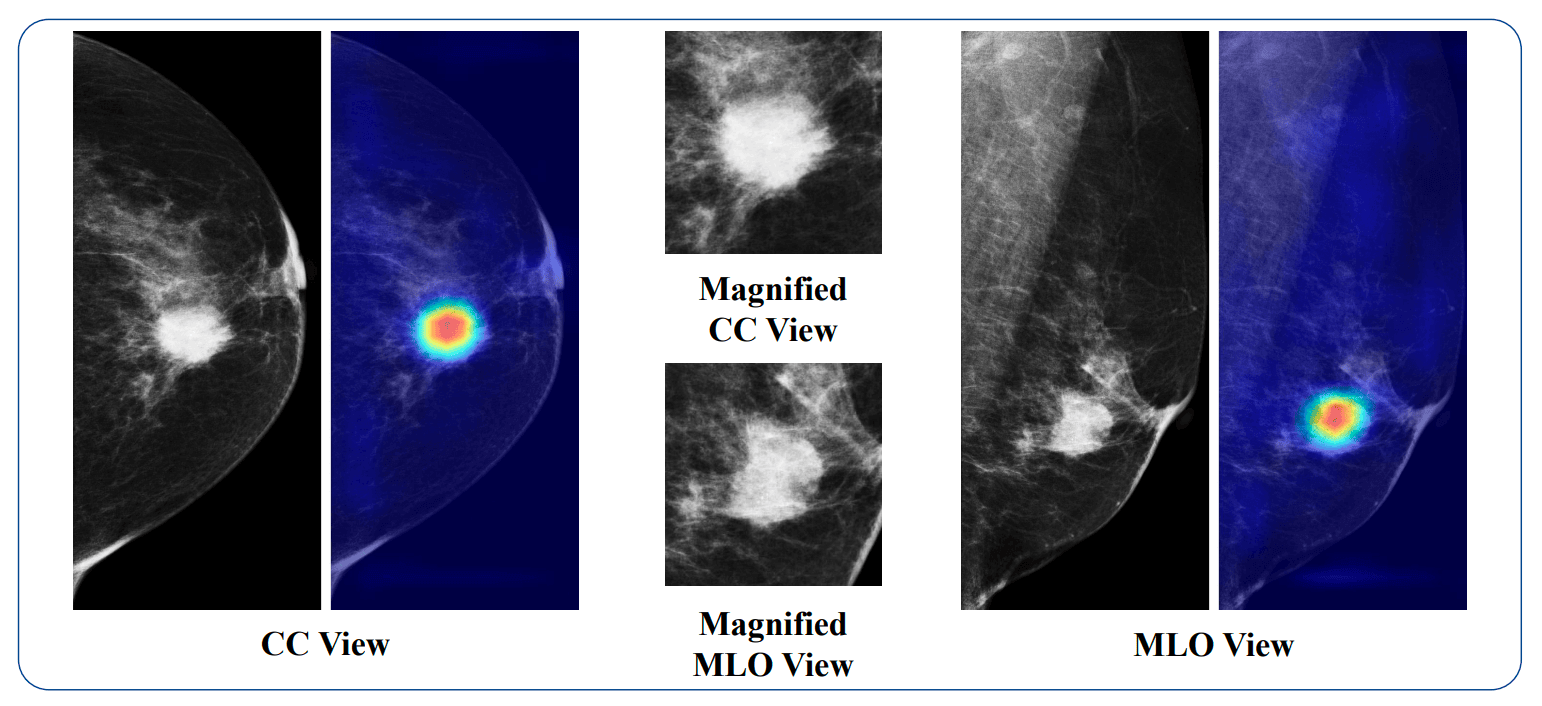
\includegraphics[width=0.8\linewidth]{reports//assets/grad-cam.png}
\caption[Grad-CAM example]{Ejemplo de la técnica Grad-CAM aplicada a una mamografía, resaltando la región correspondiente a la masa \cite{panambur_classification_2023}.}
\label{fig:grad-cam-example}
\end{figure}

\chapter{Materiales y Métodos}

Esta sección describe los materiales y métodos utilizados en este estudio. Comienza con una descripción del conjunto de datos seleccionado para el entrenamiento y análisis del modelo, luego aborda el procesamiento y la preparación de las imágenes, y concluye con las métricas de evaluación empleadas para valorar el rendimiento del modelo.

\section{La Base de Datos China de Mamografías}

La Base de Datos China de Mamografías (CMMD) es un conjunto de datos público desarrollado por Cai et al. (2023) \cite{cai_online_2023} y alojado en The Cancer Imaging Archive (TCIA)\footnote{\url{https://www.cancerimagingarchive.net/collection/cmmd/}}. Este conjunto incluye un total de 3,712 mamografías de 1,775 pacientes chinas, en vistas CC y MLO, recolectadas entre julio de 2012 y enero de 2016. CMMD se divide en dos subconjuntos:

\begin{itemize}
\item \textbf{CMMD1}: Este subconjunto incluye muestras con diagnósticos tanto malignos como benignos, junto con datos clínicos clave como la edad del paciente, tipo de anomalía y clasificación tumoral.
\item \textbf{CMMD2}: Este subconjunto contiene únicamente diagnósticos malignos, proporcionando la misma metainformación que CMMD1, pero con la adición de la clasificación del subtipo molecular para cada tumor.
\end{itemize}

La Tabla \ref{tab:cmmd_features} muestra las principales características detalladas de cada subconjunto.

\begin{table}
\caption[Características principales de los subconjuntos de CMMD]{Características principales de los subconjuntos de CMMD}
\centering
\begin{tabular}{lccccc}
\toprule
& \textbf{CMMD1} & \textbf{CMMD2} & \\
\midrule
\textbf{Número de pacientes} & 1026 & 749 & 1775 \\
\textbf{Número de mamografías} & 2230 & 1498 & 3728 \\
\textbf{Edad media del paciente} & 45.92 (17-84 años) & 49.82 (21-87 años) & - \\
\textbf{Resultado diagnóstico} & Benigno y Maligno & Maligno & - \\
\textbf{Subtipo molecular} & No & Sí & - \\
\bottomrule
\end{tabular}
\label{tab:cmmd_features}
\end{table}

\subsection{Selección del Subconjunto CMMD2}

En esta investigación, el enfoque se centra exclusivamente en el subconjunto CMMD2, ya que es el único conjunto de datos de acceso libre y público que proporciona anotaciones de subtipos moleculares. Estas anotaciones son esenciales para el entrenamiento de modelos en la clasificación de subtipos moleculares de cáncer de mama, que constituye el objetivo principal de este estudio.

\subsection{Descripción General de CMMD2}

Para la composición de CMMD2, solo se seleccionaron casos con información completa de marcadores inmunohistoquímicos y un diagnóstico confirmado de carcinoma invasivo, según se detalla en los criterios de inclusión y exclusión mostrados en la Figura~\ref{fig:cmmd_criteria}. La aplicación de estos criterios resultó en un subconjunto compuesto por 1,498 mamografías de 749 pacientes. Dado que cada paciente cuenta con vistas CC y MLO, el número total de imágenes para este subconjunto es de 2,996.

\begin{figure}[h!]
\centering
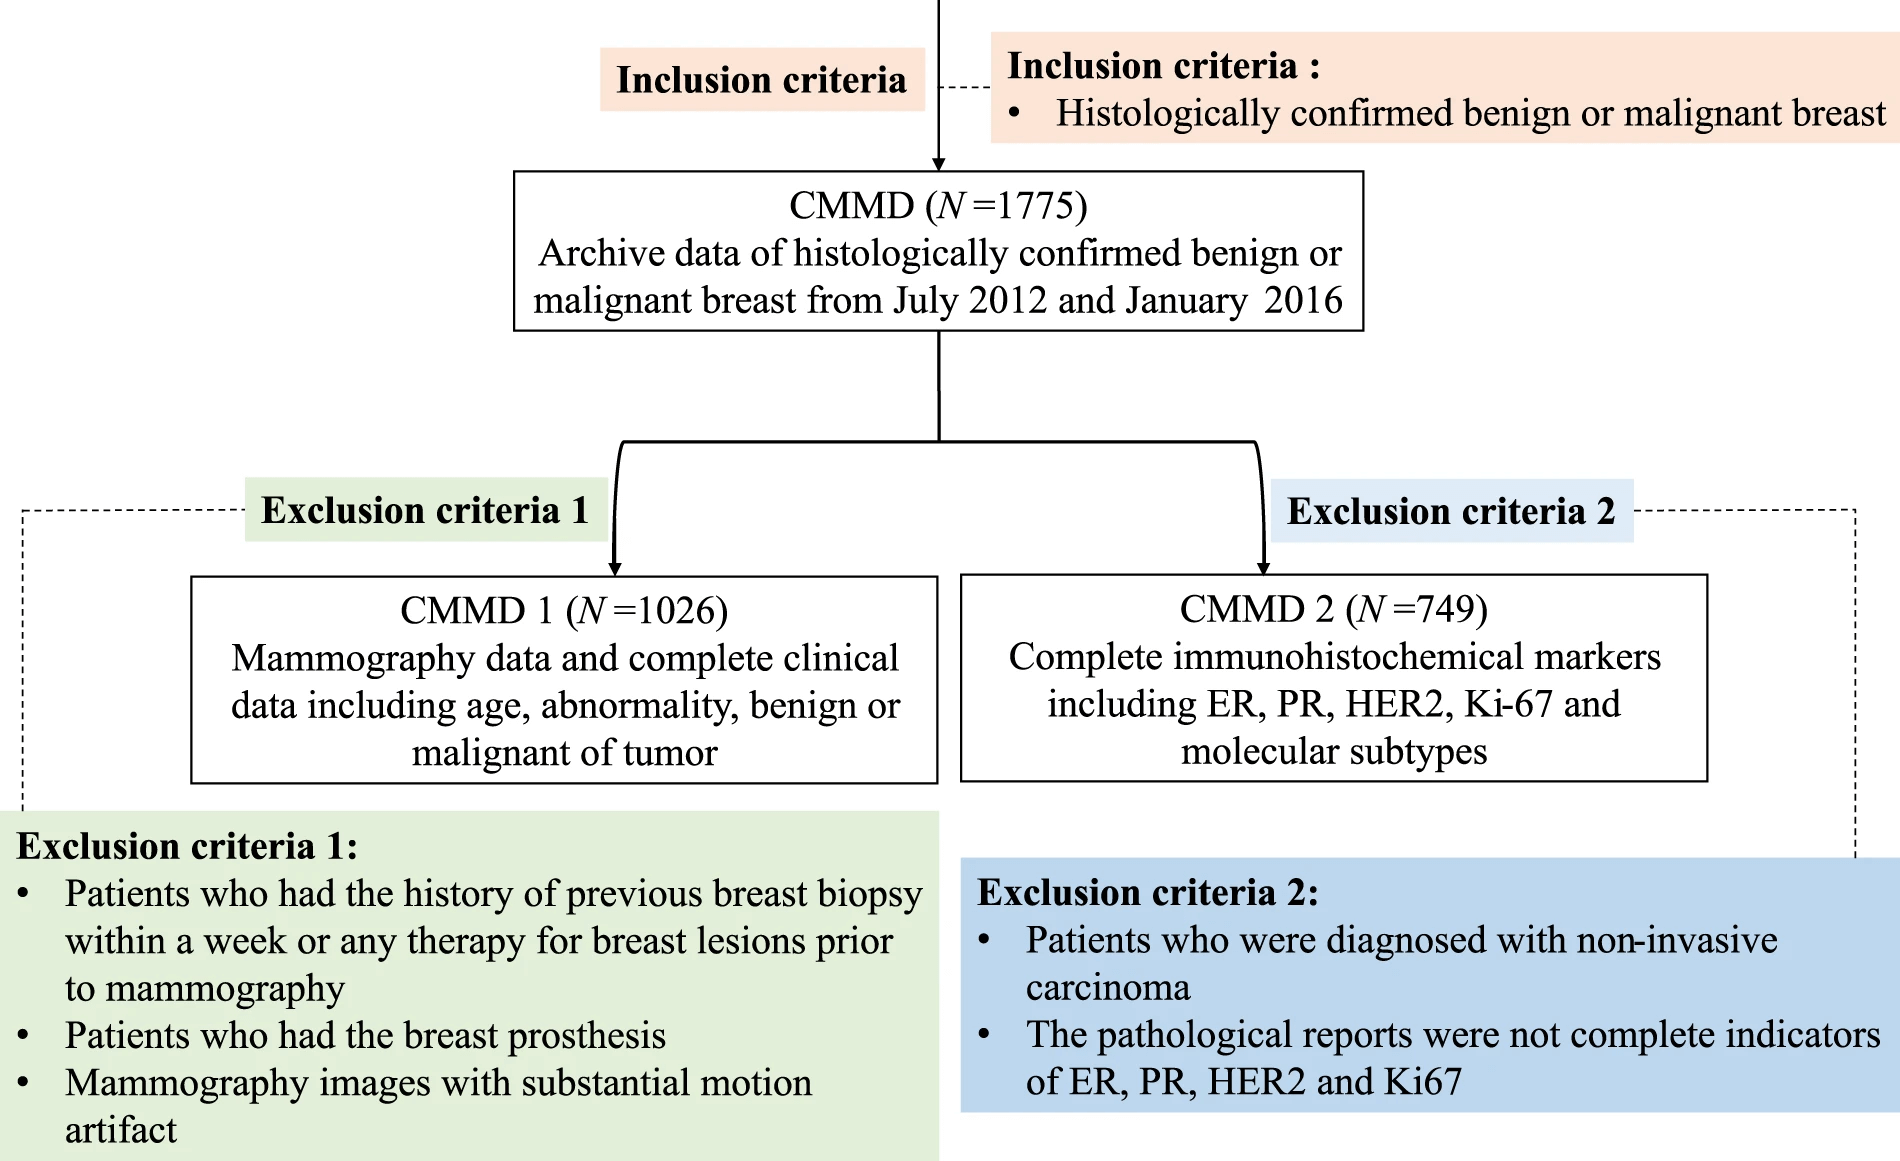
\includegraphics[width=0.85\linewidth]{reports//assets/cmmd_criteria.png}
\caption[Criterios de inclusión y exclusión de CMMD]{Criterios de inclusión y exclusión de CMMD \cite{cai_online_2023}.}
\label{fig:cmmd_criteria}
\end{figure}

\textbf{Recolección de Imágenes}

Las imágenes de mamografía se recolectaron utilizando el sistema de mamografía \textbf{GE Senographe DS}, obteniendo tanto vistas CC como MLO para cada paciente. Las imágenes se almacenaron en escala de grises de 8 bits con un tamaño de imagen de 2294×1914 píxeles \cite{cai_online_2023}.

\textbf{Formato y Resolución de las Imágenes}

El formato principal de las imágenes en el conjunto de datos es DICOM (Digital Imaging and Communications in Medicine), el estándar en imagen médica, ya que permite almacenar metadatos clínicos junto a la imagen y posibilita la interoperabilidad entre equipos de diferentes fabricantes, así como la interacción entre distintos sistemas de información en hospitales y centros de salud.

\subsection{Metadatos de CMMD2}

Para cada paciente, el conjunto de datos proporciona un archivo CSV\footnote{Un archivo de texto plano que almacena datos en forma de tabla, donde cada línea representa una fila y cada valor en la fila está separado por una coma} (Comma Separated Values) con información adicional a las imágenes obtenidas, incluyendo edad, lateralidad, tipo de anomalía, clasificación y, en el caso de CMMD2, también el subtipo molecular del tumor. La Tabla \ref{tab:cmmd2_metadata} describe estos datos en detalle.

\begin{table}[h!]
    \caption[Descripción de los metadatos de CMMD2]{Descripción de las variables de metadatos presentes en el conjunto de datos CMMD2.}
    \centering
    \begin{tabular}{>{\bfseries}l p{5cm} p{6cm}}
    \toprule
    \textbf{Columna} & \textbf{Descripción} & \textbf{Valores posibles} \\
    \midrule
    ID1 & Identificador único del paciente & Formato: D2-XXXX \\
    LeftRight & Lateralidad mamaria & L (izquierda), R (derecha) \\
    Age & Edad del paciente al momento del estudio & Entre 21 y 87 años \\
    Number & Número de imágenes disponibles por estudio & Entre 2 y 4 \\
    Abnormality & Tipo de anomalía & Masa, Calcificación, Ambas \\
    Classification & Naturaleza de la anomalía & Benigna, Maligna \\
    Subtype & Subtipo molecular del cáncer de mama & Luminal A, Luminal B, HER2-enriquecido, Triple negativo \\
    \bottomrule
    \end{tabular}

	\label{tab:cmmd2_metadata}
\end{table}

Es importante señalar que la columna de lateralidad indica el lado donde se encontró el tumor; por lo tanto, el lado opuesto se considera benigno \cite{cai_online_2023}.

La distribución de edades de los pacientes sigue una distribución aproximadamente normal con ligeras asimetrías. El rango de edad más frecuente se sitúa entre los 45 y 55 años, lo cual es coherente con la epidemiología del cáncer de mama, donde la mayoría de los casos se diagnostican en este intervalo de edad. La inclusión de pacientes más jóvenes en el conjunto de datos incrementa la diversidad poblacional y permite analizar el rendimiento del modelo en subgrupos demográficos subrepresentados. La Figura \ref{fig:age_dist_all} ilustra esta distribución.

\begin{figure}[h!]
\centering
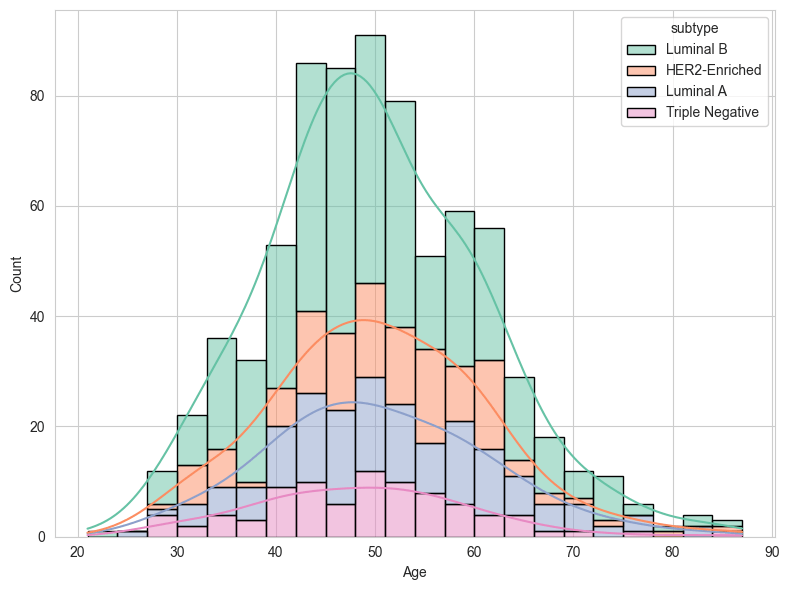
\includegraphics[width=0.5\linewidth]{reports//assets/age_dist.png}
\caption[Distribución de edad en CMMD2]{Distribución general de edad de los pacientes y subtipo molecular en CMMD2.}
\label{fig:age_dist_all}
\end{figure}

El análisis de la distribución de subtipos moleculares dentro del conjunto de datos CMMD2 también es fundamental, ya que determina la representatividad estadística de cada clase y, en consecuencia, afecta la capacidad de generalización de los modelos en escenarios clínicos. El conjunto de datos presenta un desequilibrio significativo de clases\footnote{El desequilibrio de clases se refiere a la representación desigual de diferentes clases en un conjunto de datos, donde algunas clases tienen considerablemente más o menos muestras que otras.}, siendo Luminal B el subtipo más prevalente (376 pacientes, 50.2\%), seguido de Luminal A (152 pacientes, 20.3\%), HER2-enriquecido (135 pacientes, 18.0\%) y Triple Negativo como el subtipo menos representado (86 pacientes, 11.5\%).

El desequilibrio de clases también se refleja en el número total de imágenes disponibles por subtipo, ya que cada paciente aporta al menos dos vistas mamográficas (proyecciones CC y MLO), con pocas excepciones. Este desequilibrio representa un desafío importante para los modelos de clasificación de aprendizaje automático, que tienden a mostrar sesgo hacia las clases mayoritarias cuando no se implementan estrategias adecuadas de balanceo. Sin embargo, esta distribución refleja con precisión la prevalencia relativa observada en la práctica clínica, donde los subtipos Luminales (A y B) son los más comunes, mientras que el cáncer de mama Triple Negativo representa aproximadamente el 10-15\% de todos los casos.

\begin{figure}[h!]
\centering
\begin{subfigure}[t]{0.49\textwidth}
\centering
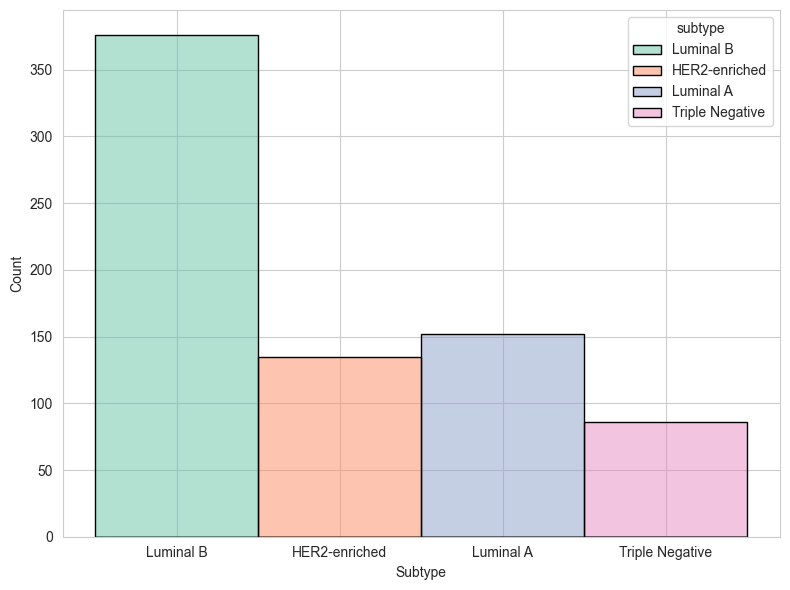
\includegraphics[width=\textwidth]{reports//assets/hist.png}
\caption{Distribución de subtipos}
\label{fig:subtype_hist}
\end{subfigure}
\begin{subfigure}[t]{0.49\textwidth}
\centering
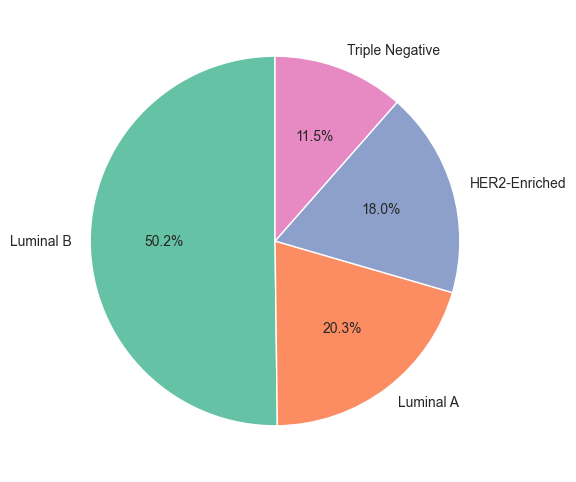
\includegraphics[width=\textwidth]{reports/assets/pie.png}
\caption{Distribución de subtipos (gráfico circular)}
\label{fig:subtype_pie}
\end{subfigure}
\caption[Distribución de subtipos moleculares en CMMD2]{Distribución de subtipos de pacientes (CMMD2)}
\label{fig:subtype_charts}
\end{figure}

\subsection{Limitaciones y Desafíos de CMMD2}

Aunque CMMD2 es un conjunto de datos valioso para este estudio, presenta ciertas limitaciones que deben tenerse en cuenta:

\begin{enumerate}
\item \textbf{Falta de anotaciones de región de interés (ROI)}: El conjunto de datos no proporciona ROIs anotadas para las ubicaciones tumorales, lo que dificulta que los modelos de aprendizaje automático se centren en las áreas relevantes dentro de las imágenes.
\item \textbf{Proveedor único de imágenes}: Todas las mamografías fueron adquiridas utilizando el mismo dispositivo de imagen. Como resultado, los modelos entrenados con este conjunto pueden no generalizar bien a imágenes obtenidas de diferentes dispositivos o proveedores.
\item \textbf{Alto desequilibrio de clases}: Como se mencionó anteriormente, el conjunto de datos sufre un desequilibrio significativo de clases. Esto puede provocar que los modelos se sobreajusten a la clase dominante, aunque refleja la distribución real de los subtipos moleculares de cáncer de mama.
\end{enumerate}

\subsection{Ejemplos de Imágenes de CMMD2}

\begin{figure}[h!]
\centering
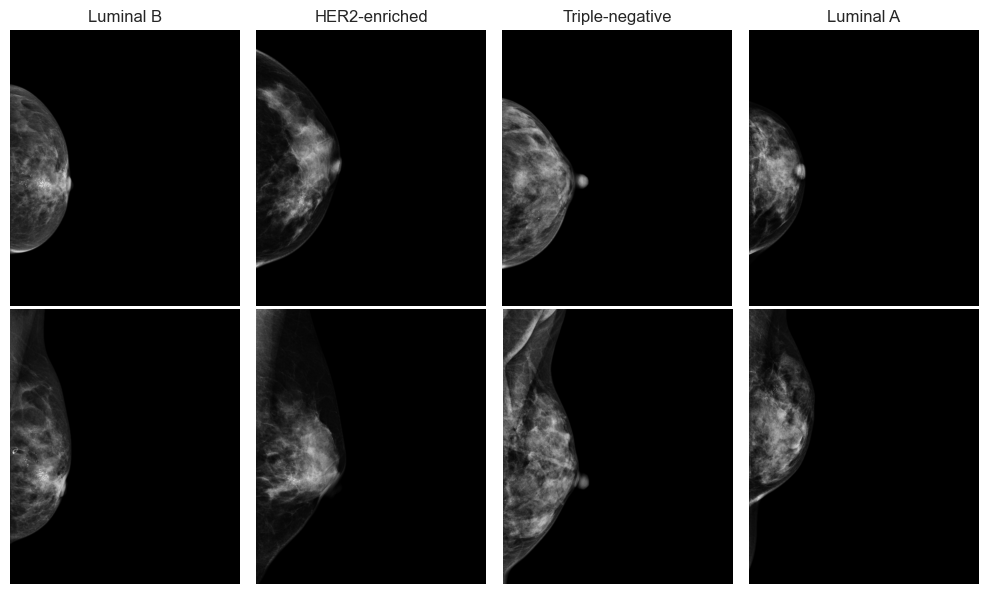
\includegraphics[width=1.0\linewidth]{reports//assets/images_examples.png}
\caption[Ejemplos de imágenes de mamografía de CMMD2]{Ejemplo de imágenes de mamografía del conjunto de datos CCMD2. La fila superior representa una vista CC, mientras que la fila inferior ilustra una vista MLO. Cada columna representa un subtipo de cáncer.}
\label{fig:cmmd-examples}
\end{figure}

\section{El análisis TOMPEI-CMMD}

TOMPEI-CMMD es un análisis mejorado del conjunto de datos original CMMD, desarrollado por Kashiwada et al. (2025) \cite{kashiwada_tompei-cmmd_2025}. Esta mejora fue diseñada para proporcionar información radiológica integral y permitir una reevaluación sistemática de las imágenes mamográficas existentes.

Un radiólogo certificado, con 20 años de experiencia en imagen mamaria, evaluó todas las imágenes, documentando hallazgos radiológicos detallados, incluyendo masas, calcificaciones, densidades focales asimétricas, distorsiones arquitectónicas y sus localizaciones anatómicas. Este nuevo análisis también proporciona máscaras de segmentación a nivel de píxel para todos los hallazgos identificados en las vistas MLO, generadas a partir de la evaluación experta del radiólogo.

TOMPEI-CMMD es valioso para este estudio porque también aporta información adicional sobre los datos del subconjunto CMMD2, específicamente en lo referente a exclusiones de mamografías y correcciones de lateralidad guiadas por el radiólogo experto. Estas mejoras permiten una curación adicional del conjunto de datos CMMD2, mejorando su calidad.

La Tabla~\ref{tab:tompei_exclusions} resume los motivos de exclusión identificados durante el análisis TOMPEI-CMMD, así como el número de elementos afectados en el subconjunto CMMD2.

\begin{table}[h!]
\caption[Motivos de exclusión en TOMPEI-CMMD]{Número de mamografías de CMMD2 afectadas por cada motivo de exclusión según el análisis TOMPEI-CMMD.}
\centering
\begin{tabular}{l p{6cm} c}
\toprule
\textbf{Motivo de exclusión} & \textbf{Descripción} & \textbf{Mamografías afectadas} \\
\midrule
CV Port & Presencia de un puerto venoso central visible en la imagen de mamografía. & 7 \\
Linfedema & Presencia de cambios relacionados con linfedema visibles en la imagen. & 1 \\
Neurofibromatosis & Presencia de hallazgos relacionados con neurofibromatosis visibles en la imagen. & 2 \\
Objetos blancos & Presencia de objetos blancos extraños o artefactos en la imagen. & 2 \\
Invisible & Lesión no visible o indetectable en la imagen de mamografía. & 76 \\
Benigno & Lesión determinada como benigna tras la revisión experta. & 10 \\
Normal & No se detectaron hallazgos anormales en la imagen. & 724 \\
\textbf{Total} & & \textbf{824} \\
\bottomrule
\end{tabular}
\label{tab:tompei_exclusions}
\end{table}

Después de aplicar todas las exclusiones y realizar 9 correcciones de lateralidad (donde las imágenes estaban mal etiquetadas), nuestro conjunto de datos final se resume en la Tabla~\ref{tab:final_dataset_overview}.

\begin{table}[h!]
\caption[Resumen del conjunto de datos final]{Resumen del conjunto de datos final tras exclusiones y correcciones.}
\centering
\begin{tabular}{c c c}
\toprule
\textbf{Pacientes} & \textbf{Mamografías} & \textbf{Imágenes} \\
\midrule
672 & 674 & 1348 \\
\bottomrule
\end{tabular}
\label{tab:final_dataset_overview}
\end{table}

En el conjunto de datos final hay 672 pacientes únicos. Sin embargo, dos pacientes fueron diagnosticados con cáncer de mama bilateral\footnote{Cáncer en ambas mamas, izquierda y derecha.}, lo que da como resultado un total de 674 mamografías. Como cada mamografía incluye tanto la vista CC como la MLO, el conjunto de datos final incluye 1,348 imágenes.

\section{Preprocesamiento de Imágenes}

Para preparar el conjunto de datos para experimentos de aprendizaje profundo, el preprocesamiento de imágenes es esencial. Las imágenes originales se almacenan en formato DICOM (\texttt{.dcm}), y muchas incluyen un fondo negro sustancial, lo que puede afectar negativamente tanto la eficiencia computacional como el rendimiento del modelo si no se corrige.

Se aplicaron los siguientes pasos de preprocesamiento, y el resultado final se ilustra en la Figura~\ref{fig:preprocessing}:

\begin{enumerate}
\item \textbf{Recorte Inteligente}: Se aplicó un algoritmo heurístico\footnote{Un enfoque práctico basado en reglas diseñado para encontrar rápidamente una buena solución a un problema cuando encontrar la solución óptima sería demasiado complejo o llevaría demasiado tiempo.} para recortar automáticamente la mayor parte del fondo negro de cada imagen, conservando solo la región que contiene tejido mamario. Este paso maximiza el enfoque del modelo en las estructuras anatómicas relevantes y reduce la carga computacional.
\item \textbf{Filtrado Mediano}: Se utilizó un filtro mediano para reducir el ruido mientras se preservan los bordes y detalles importantes en las mamografías. Esto ayuda a mejorar la calidad de la imagen y favorece una extracción de características más fiable por parte de los modelos de aprendizaje profundo.
\item \textbf{Conversión y Almacenamiento de Imágenes}: Las imágenes preprocesadas se convirtieron a un formato estándar (PNG) y se almacenaron en un directorio más accesible. Este paso también facilita la carga eficiente de datos y la reproducibilidad en experimentos posteriores.
\end{enumerate}

\begin{figure}[h!]
\centering
\begin{subfigure}[t]{0.35\textwidth}
\centering
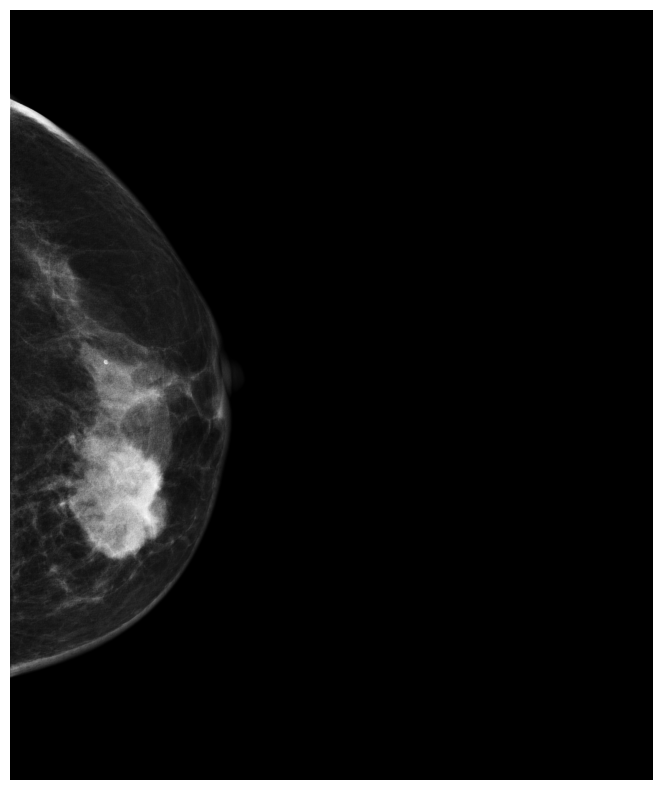
\includegraphics[width=\textwidth]{reports//assets/preprocess_a.png}
\caption{}
\label{fig:pre_original}
\end{subfigure}
\begin{subfigure}[t]{0.15\textwidth}
\centering
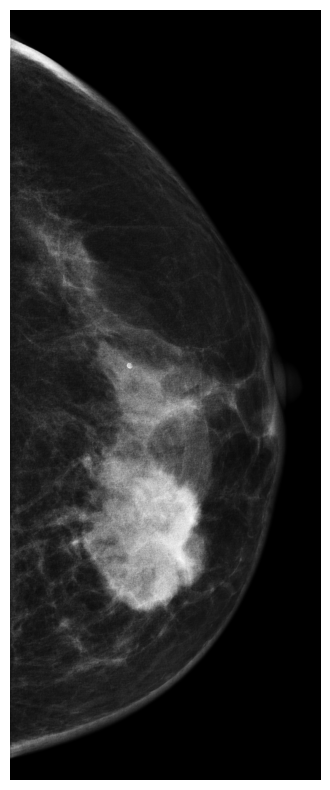
\includegraphics[width=\textwidth]{reports//assets/preprocess_b.png}
\caption{}
\label{fig:pre_cropped}
\end{subfigure}
\begin{subfigure}[t]{0.15\textwidth}
\centering
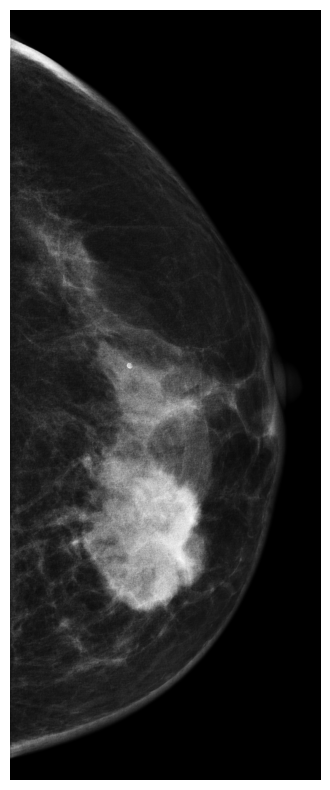
\includegraphics[width=\textwidth]{reports//assets/preprocess_c.png}
\caption{}
\label{fig:pre_mean}
\end{subfigure}
\caption[Resultado del flujo de preprocesamiento]{Ilustración del resultado del flujo de preprocesamiento: (a) imagen original, (b) imagen tras el recorte y (c) imagen tras la aplicación del filtro mediano.}
\label{fig:preprocessing}
\end{figure}

Después de aplicar este flujo de preprocesamiento, la estructura resultante de directorios es la siguiente. Cada imagen se almacena dentro de una carpeta etiquetada con la identificación correspondiente al paciente:

\vspace{0.5cm}
\dirtree{%
.1 data/.
.2 preprocessed.
.3 D2-0001.
.4 CC-L.png.
.4 MLO-L.png.
.3 D2-0002.
.3 ....
}

Además de estos pasos de preprocesamiento, también se aplica una técnica de estandarización de histograma\footnote{La estandarización de histograma es una técnica utilizada para ajustar los valores de intensidad de una imagen de modo que su histograma tenga una media y varianza especificadas, generalmente media 0 y varianza 1. Esto ayuda a que las imágenes de diferentes fuentes sean más comparables y consistentes para análisis posteriores.}. Sin embargo, esto se realiza durante la fase de partición de datos para evitar la fuga de datos\footnote{Cuando información que no estaría disponible en el momento de la predicción se utiliza involuntariamente durante el entrenamiento del modelo. Esto conduce a un rendimiento excesivamente optimista durante la evaluación, pero a malos resultados en el uso real, porque el modelo ha aprendido patrones a los que no debería tener acceso.}. Los detalles sobre este procedimiento se discutirán en la siguiente sección.

\section{División y Estratificación de los Datos}

Una vez preprocesadas las imágenes, el siguiente paso es crear particiones de entrenamiento y prueba del conjunto de datos. En aprendizaje profundo, es una práctica estándar dividir el conjunto de datos en subconjuntos separados para evaluar con precisión el rendimiento del modelo y prevenir el sobreajuste, asegurando que el modelo generalice bien a datos no vistos \cite{noauthor_data_nodate}. En particular, deben abordarse tres puntos clave:

\begin{itemize}
\item Asegurar la reproducibilidad de los experimentos.
\item Mantener la misma distribución de datos en las particiones (estratificación) para garantizar una representación equilibrada de las clases.
\item Evitar la fuga de datos asegurando que ninguna información del conjunto de prueba se utilice durante el entrenamiento.
\end{itemize}

\subsection{Estrategia de Holdout Repetido}

Para evaluar mejor el rendimiento del modelo, se utilizó la estrategia de holdout repetido. También conocida como validación cruzada Monte Carlo, este enfoque consiste en dividir aleatoriamente el conjunto de datos en conjuntos de entrenamiento y prueba múltiples veces, resultando en diferentes particiones para cada iteración. El modelo se entrena y evalúa en cada partición, y los resultados se promedian para proporcionar una estimación más robusta del rendimiento \cite{marzbanAllModelsAre2020}.

En este estudio, \textbf{se utilizaron tres particiones diferentes de entrenamiento y prueba, consistentes en 80\% de datos para entrenamiento y 20\% para prueba}. Cada partición se generó con una semilla aleatoria fija diferente (0, 21 y 42) para asegurar la reproducibilidad del proceso de partición de datos. Para mayor claridad, cada partición se nombra según su semilla correspondiente (por ejemplo, Split 0).

\subsection{Distribución de los Datos}

Para asegurar una distribución de datos consistente entre las diferentes particiones de entrenamiento y prueba, se realizó una estratificación basada en las anotaciones de subtipo molecular. Esto garantizó que cada partición de entrenamiento y prueba mantuviera una proporción similar de cada subtipo molecular, reduciendo así el riesgo de estimaciones sesgadas del rendimiento debido al desequilibrio de clases. Las distribuciones de datos resultantes para las tres particiones se muestran en la Figura~\ref{fig:pie_dist} y la Figura~\ref{fig:pie_hist}, junto con información adicional sobre el solapamiento de imágenes.

\subsection{Prevención de Fuga de Datos}

Para evitar la fuga de datos, las particiones se realizaron a nivel de paciente. Esto significa que se utilizó la identificación del paciente para asegurar que todas las muestras de un mismo paciente se asignaran exclusivamente al conjunto de entrenamiento o al de prueba, evitando cualquier solapamiento entre ambos. Esta consideración se incluyó en el entrenamiento, donde el uso de un Stratified Grouped K-Fold garantizó que no hubiera fuga de datos de pacientes entre los folds.

\subsection{Estandarización de Histograma}

La estandarización de histograma es un paso importante de preprocesamiento que iguala las intensidades de las imágenes para reducir la variabilidad, incluso dentro de conjuntos de datos adquiridos con un solo dispositivo como CMMD2. Se ha demostrado que esta técnica mejora la generalización entre dominios y el rendimiento del modelo \cite{garruchoDomainGeneralizationDeep2022}. En este estudio, la estandarización de histograma se aplicó después de la partición de datos, siguiendo la estrategia de holdout repetido. Para cada partición de entrenamiento y prueba, los puntos de referencia de intensidad se aprendieron a partir del conjunto de entrenamiento y luego se aplicaron para estandarizar tanto las imágenes de entrenamiento como las de prueba. Un ejemplo del efecto de esta técnica en el aspecto de la imagen y la distribución de intensidades se muestra en la Figura~\ref{fig:standardized_examples}.


\begin{figure}[h!]
    \centering
    \begin{subfigure}[t]{1.0\textwidth}
        \centering
        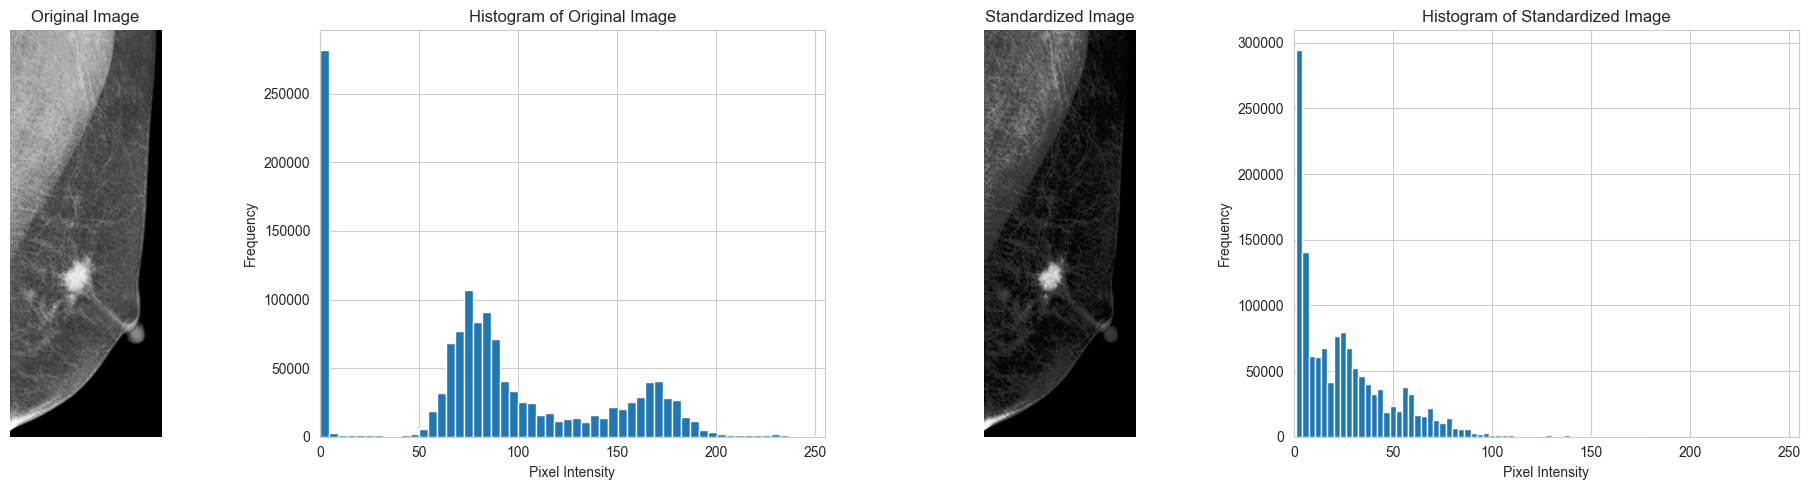
\includegraphics[width=\textwidth]{reports//assets/standarized1.png}
        \label{fig:standarized_1}
    \end{subfigure}
    \begin{subfigure}[t]{1.0\textwidth}
        \centering
        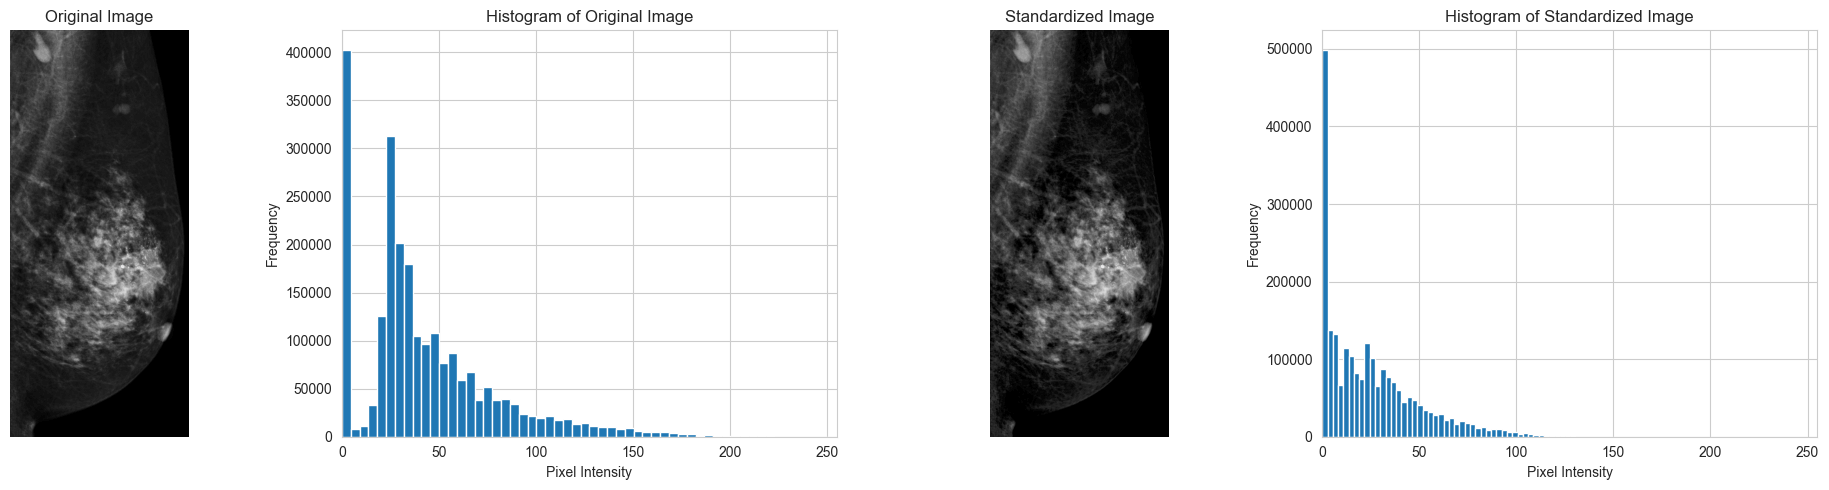
\includegraphics[width=\textwidth]{reports//assets/standarized2.png}
        \label{fig:standardized_2}
    \end{subfigure}
    \caption[Resultado de la estandarización de histograma]{Ejemplo de una imagen antes y después de aplicar la estandarización de histograma. Los histogramas demuestran cómo las distribuciones de intensidad se vuelven más similares tras la estandarización.}
    \label{fig:standardized_examples}
\end{figure}

\subsection{Resumen de las particiones finales}

Tras el preprocesamiento, la división de datos y la estandarización de histograma, las imágenes se organizaron sistemáticamente por semilla, partición y subtipo para permitir una carga eficiente de datos durante el entrenamiento. El formato final de imagen seleccionado fue \texttt{.npy}\footnote{Formato binario de NumPy}, debido a su capacidad para un almacenamiento eficiente, carga rápida de grandes arreglos y preservación exacta de los valores de intensidad, incluyendo los rangos estandarizados de histograma, sin pérdida ni alteración.

La estructura de directorios de las particiones se presenta a continuación:

\vspace{0.5cm}
\dirtree{%
.1 splits/.
.2 SEED0.
.3 train.
.4 her2-enriched.
.5 D2-0001-CC-R.npy.
.4 luminal-a.
.4 luminal-b.
.4 triple-negative.
.3 test.
.2 SEED21.
.2 SEED42.
}

\section{Métricas de Evaluación}

Seleccionar métricas de evaluación apropiadas es esencial para valorar con precisión el rendimiento del modelo, especialmente en tareas de clasificación multiclase como la diferenciación de subtipos moleculares de cáncer de mama. Para asegurar la coherencia con estudios recientes, como los de Mota et al \cite{mota_breast_2024} y Rabah et al \cite{ben_rabah_multimodal_2025}, este trabajo reporta métricas como AUC, Precisión, Recall y F1-Score, haciendo énfasis en los valores promediados macro. El macro-promedio trata a cada clase por igual, promediando las métricas calculadas de forma independiente para cada clase, lo cual es especialmente importante dada la alta desproporción de clases en el conjunto de datos.

Adicionalmente, se incluye el coeficiente Kappa de Cohen para medir el acuerdo entre las etiquetas predichas y las verdaderas, teniendo en cuenta el azar. Para abordar aún más el desequilibrio de clases, se reporta la Precisión Balanceada en lugar de la precisión estándar. Para la visualización de métricas, se utilizó la curva ROC AUC para comparar los resultados globales de esta métrica y una matriz de confusión \cite{noauthor_que_nodate} para evaluar las predicciones.

La Tabla \ref{tab:metrics_overview} resume las métricas de evaluación utilizadas en este estudio:

\begin{table}[h!]
\centering
\caption[Resumen de Métricas]{Resumen de las métricas de evaluación utilizadas en este trabajo. Todas las métricas, excepto AUC y Kappa de Cohen, se reportan como valores promediados macro.}
\begin{tabularx}{\textwidth}{l X X}
\toprule
\textbf{Metric} & \textbf{Formula} & \textbf{Description} \\
\midrule
    Balanced Accuracy &
$\frac{1}{N}\sum_{i=1}^N \frac{TP_i}{TP_i + FN_i}$ &
Promedio del recall en todas las clases; robusta frente al desequilibrio de clases. \\
Macro Precisión &
$\frac{1}{N}\sum_{i=1}^N \frac{TP_i}{TP_i + FP_i}$ &
Promedio de la precisión por clase; trata todas las clases por igual. \\
Macro Recall (Sensibilidad) &
$\frac{1}{N}\sum_{i=1}^N \frac{TP_i}{TP_i + FN_i}$ &
Promedio del recall por clase; trata todas las clases por igual. \\
Macro F1-Score &
$\frac{1}{N}\sum_{i=1}^N 2 \cdot \frac{\text{Precision}_i \cdot \text{Recall}_i}{\text{Precision}_i + \text{Recall}_i}$ &
Promedio de los F1-score por clase; equilibra precisión y recall. \\
Kappa de Cohen &
$\frac{p_o - p_e}{1 - p_e}$ &
Mide el acuerdo entre las predicciones y las etiquetas verdaderas, ajustado por azar. \\
Macro AUC (ROC) &
--- &
Área promedio bajo la curva ROC para cada clase; mide la capacidad de distinguir entre clases. \\
\bottomrule
\end{tabularx}
\label{tab:metrics_overview}
\end{table}

\section{Arquitecturas de Modelos y Pipeline}

\subsection{Selección de Backbones de Modelos}

Para este estudio, las arquitecturas de modelos (backbones) se seleccionaron utilizando la librería \textit{timm} \cite{TimmPyTorchImage2025}, que proporciona una amplia variedad de modelos preentrenados de última generación para clasificación de imágenes.

\begin{itemize}
    \item \textbf{ResNet-101}: timm/resnet101
    \item \textbf{ViT}: timm/vit\_base\_patch16\_384
    \item \textbf{MaxVit}: timm/maxvit\_small\_tf\_384
    \item \textbf{Swin}: timm/swin\_base\_patch4\_window12\_384
\end{itemize}

\subsection{Formato de Entrada de los Modelos}

Definir la forma de entrada es esencial al trabajar con modelos preentrenados, ya que normalmente se entrenan en conjuntos de datos de referencia con tamaños de entrada fijos como 224×224, 384×384 o 512×512. Para asegurar una comparación justa entre las cuatro arquitecturas, estandarizamos el tamaño de entrada a 384×384×3 (RGB). Esta decisión está respaldada por evidencia empírica que muestra que los modelos basados en transformers logran un rendimiento óptimo a resoluciones más altas, mientras que las CNN como ResNet101 son flexibles y también se benefician de imágenes de mayor tamaño.

Dado que el conjunto de datos no proporciona anotaciones de región de interés (ROI), como se mencionó anteriormente, aplicamos una pipeline de transformación que primero redimensiona cada imagen para que su dimensión más pequeña coincida con 384 píxeles, preservando la relación de aspecto original, y luego aplica un recorte centrado para obtener un parche de 384×384. Este enfoque sencillo es efectivo en la práctica y se ilustra en la Figura~\ref{fig:384_patches}.

\begin{figure}[h!]
    \centering
    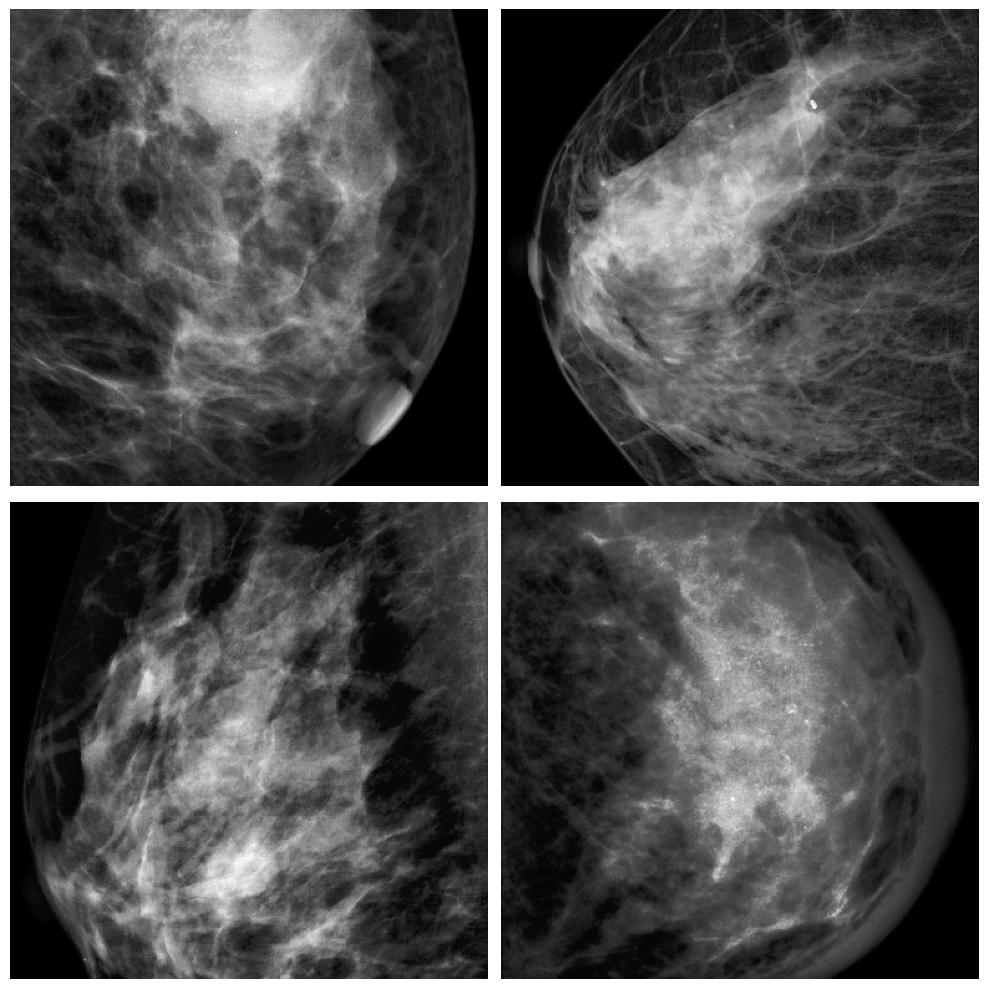
\includegraphics[width=0.3\linewidth]{reports//assets/384patchs.png}
    \caption[Parche de entrada 384×384]{Ejemplos de parches centrados de 384×384 extraídos de las imágenes originales, que luego se convierten en tensores para la entrada al modelo.}
    \label{fig:384_patches}
\end{figure}

\subsection{Formato de Salida del Modelo}

Tras procesar una imagen de entrada, cada modelo produce un tensor unidimensional que contiene las probabilidades predichas para cada uno de los cuatro subtipos moleculares. Esto significa que para cada imagen, el modelo asigna una probabilidad a cada subtipo, reflejando su confianza en la clasificación. Estas probabilidades se calculan utilizando una función de activación softmax en la capa final, asegurando que todos los valores sumen uno y puedan interpretarse como probabilidades reales. El subtipo con la mayor probabilidad es seleccionado como la predicción final del modelo para ese caso.

Al adoptar este formato de salida estandarizado en todos los modelos, se facilita la comparación directa de sus predicciones y la aplicación de métricas de evaluación consistentes. Este enfoque no solo agiliza el análisis, sino que también garantiza que las diferencias de rendimiento puedan atribuirse a los propios modelos y no a variaciones en el procesamiento de la salida. La Figura~\ref{fig:flowchart} proporciona una visión general del proceso de inferencia, desde la entrada de la imagen hasta la predicción final del subtipo.

\begin{figure}[h!]
    \centering
    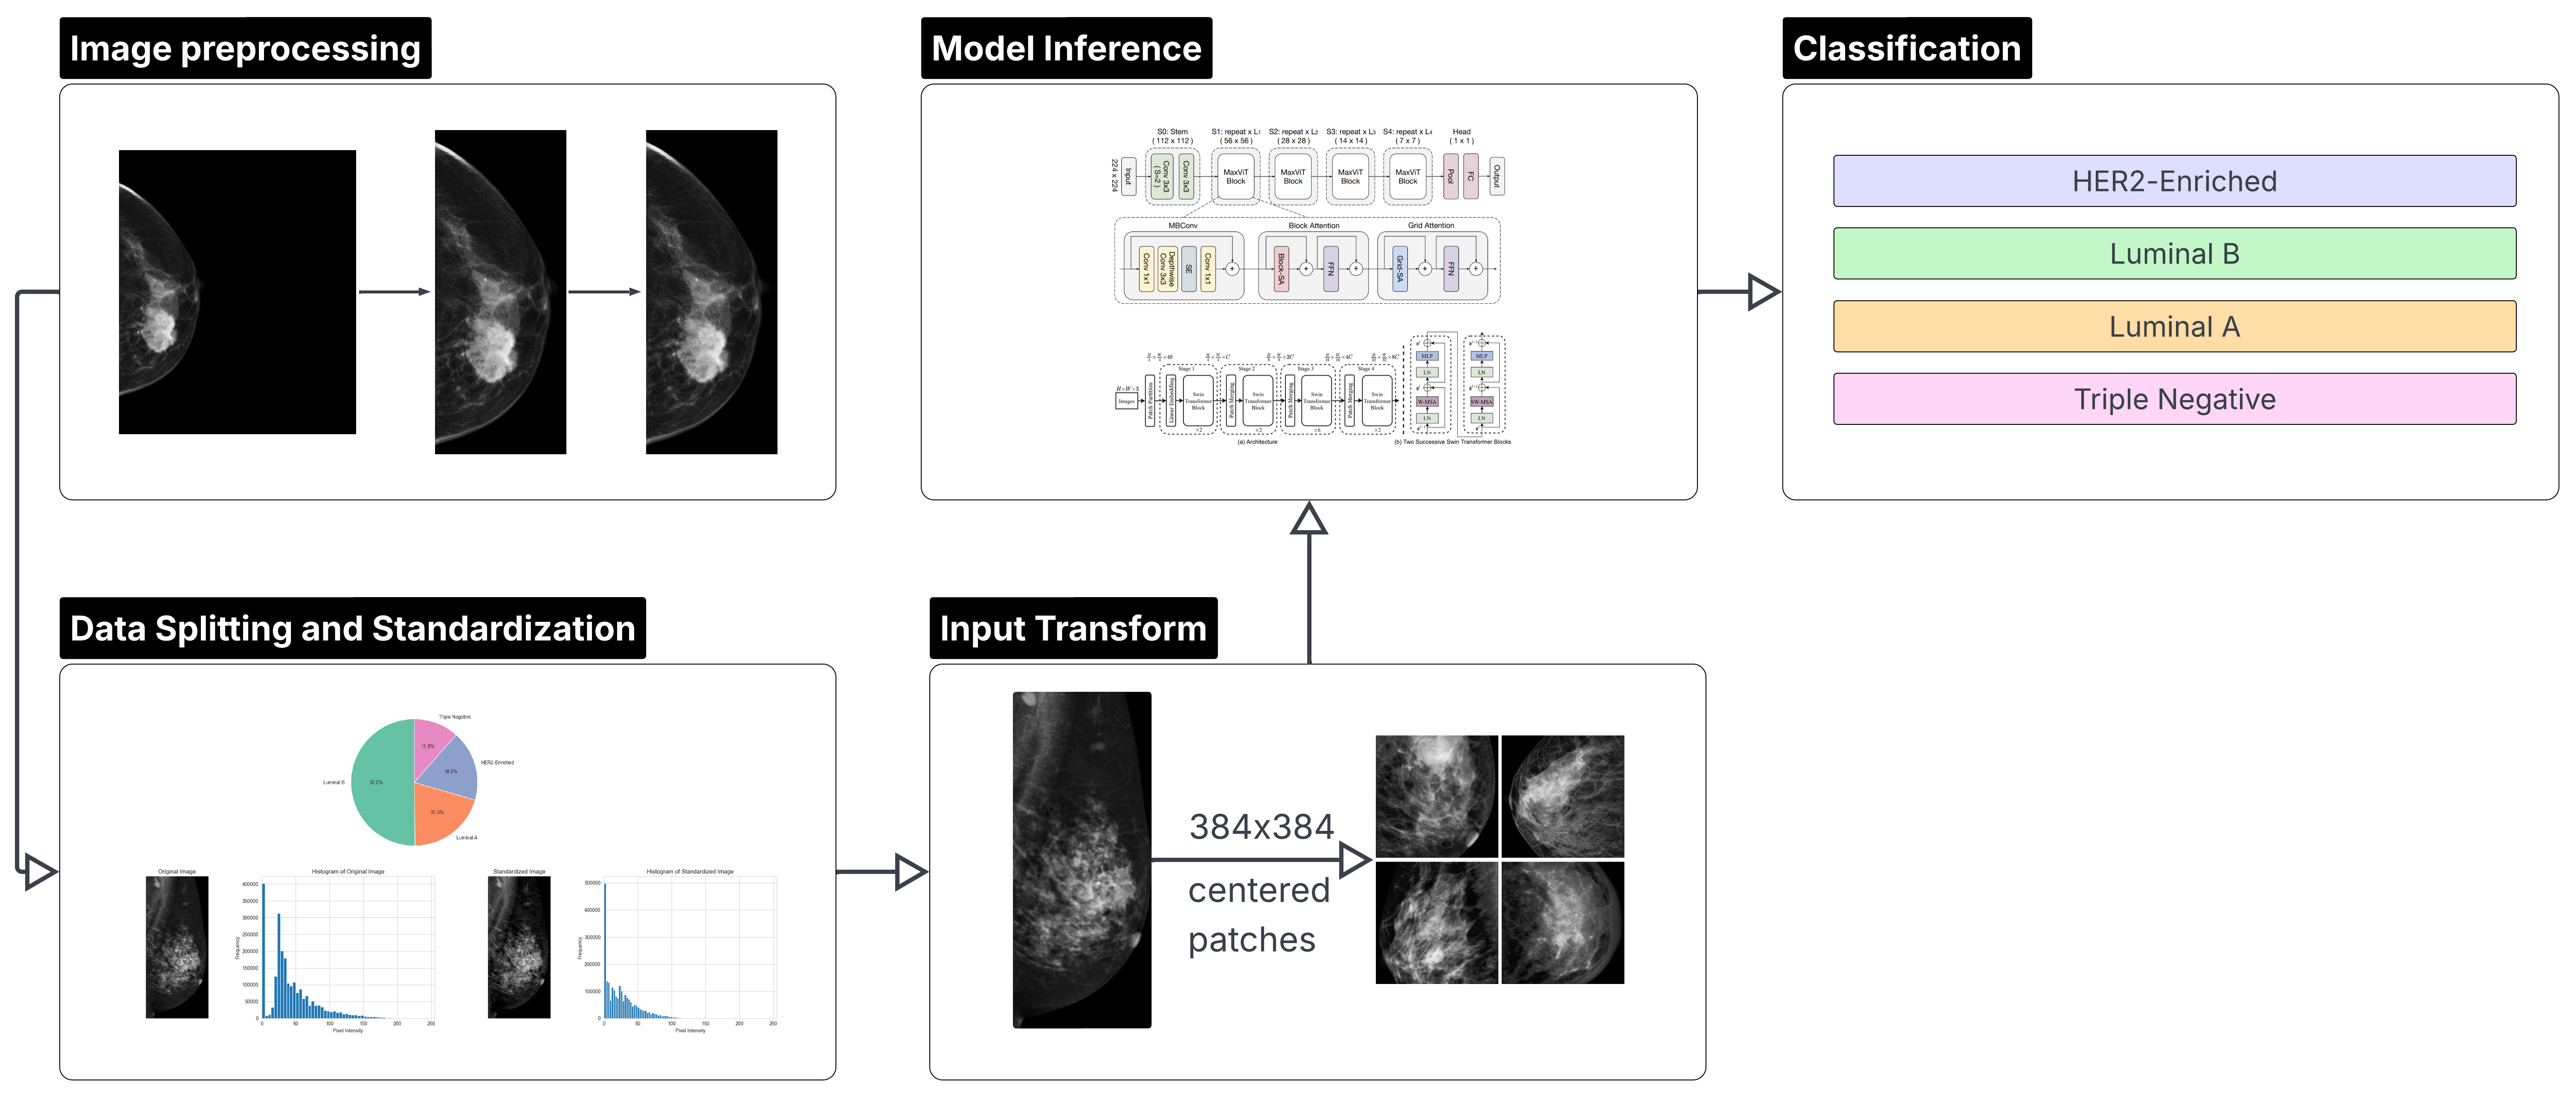
\includegraphics[width=0.9\linewidth]{reports//assets/Flowchart.png}
   \caption[Pipeline de trabajo]{Visión general del pipeline de trabajo para la inferencia del modelo tras el entrenamiento y la evaluación.}
    \label{fig:flowchart}
\end{figure}

\section{Experimentos}

Esta sección presenta el diseño experimental empleado para comparar el rendimiento de los cuatro modelos (ResNet-101, ViT, Swin y MaxViT). Se detallan las directrices y configuraciones comunes aplicadas en todos los experimentos, junto con las diferentes modalidades evaluadas usando tres particiones distintas de entrenamiento y prueba.

\subsection{Pipeline de Evaluación}

Para evaluar sistemáticamente el rendimiento de los modelos en la clasificación de subtipos moleculares de cáncer de mama, se propusieron cuatro modalidades de entrenamiento. Cada modalidad está diseñada para abordar y mitigar el desequilibrio de clases en el conjunto de datos de la forma más efectiva posible:

\begin{itemize}
\item Pérdida ponderada sin aumento de imágenes
\item Pérdida ponderada con aumento de imágenes
\item Sobremuestreo sin aumento de imágenes
\item Sobremuestreo con aumento de imágenes
\end{itemize}

Cada modalidad se aplica a los cuatro modelos utilizando una estrategia de validación cruzada de 3 folds sobre el conjunto de entrenamiento, y este proceso se repite para cada una de las tres particiones de entrenamiento y prueba. Las métricas de validación de la validación cruzada se recopilan y resumen para cada partición, proporcionando la base para el análisis estadístico posterior. Con base en los resultados de este análisis, se seleccionan las modalidades de entrenamiento con mejor rendimiento para el ajuste fino sobre todo el conjunto de entrenamiento, seguido de la evaluación en el conjunto de prueba correspondiente para cada partición. En total, la evaluación requirió \textbf{144 experimentos}, calculados como 4 modelos × 3 folds × 4 modalidades × 3 particiones de entrenamiento y prueba. El pipeline general se puede resumir de la siguiente manera:

\begin{enumerate}[label=\textbf{Paso \arabic*}:]
\item Seleccionar una partición de entrenamiento y prueba (por ejemplo, SPLIT0).
\item Seleccionar un backbone de modelo (ResNet-101, ViT, Swin o MaxViT).
\item Evaluar el modelo usando cada una de las cuatro modalidades de entrenamiento con validación cruzada de 3 folds.
\item Recopilar las métricas de validación para cada modalidad, semilla, modelo y fold.
\item Repetir el proceso para todas las particiones y modelos.
\end{enumerate}

\subsection{Hiperparámetros Comunes}

Se seleccionó un conjunto de hiperparámetros de entrenamiento comunes para asegurar que fueran adecuados para todos los tipos de modelos evaluados en este estudio. La Tabla~\ref{tab:hyperparams} resume los hiperparámetros utilizados.


\begin{table}[h!]
    \caption[Hiperparámetros comunes de entrenamiento.]{Hiperparámetros comunes de entrenamiento.}
    \centering
    \begin{tabular}{l l}
        \toprule
        \textbf{Hiperparámetros} & \textbf{Valor} \\
        \midrule
        Optimizador  & AdamW \\
        Tasa de aprendizaje  & 1e-4 (1e-5 for fine-tuning) \\
        Weight Decay (L2-Regularización) & 1e-2 \\
        Programador de LR & OneCycleLR \\
        Tamaño de Batch & 32 \\
        Épocas & 100 (máx) \\
        \bottomrule
    \end{tabular}
    \label{tab:hyperparams}
\end{table}

\subsection{Modalidades del Experimento}

\subsubsection{Uso de aumento de imágenes}

El aumento de imágenes es una técnica utilizada para incrementar la diversidad y el tamaño de un conjunto de datos generando versiones modificadas de las imágenes existentes en memoria mediante diversas transformaciones o ajustes de contraste~\cite{noauthor_complete_nodate}. Para el entrenamiento de los modelos, solo se aplicaron transformaciones leves, incluyendo volteo horizontal (50\%), rotaciones entre $-10^\circ$ y $10^\circ$ (30\%), y CLAHE (10\%)\footnote{Contrast Limited Adaptive Histogram Equalization, una técnica avanzada de procesamiento de imágenes utilizada para mejorar el contraste local de la imagen.}. Estas aumentaciones son seguras desde el punto de vista médico y ayudan a que los modelos generalicen mejor y mitiguen el desequilibrio de clases. La Figura \ref{fig:augmentations} ilustra estos aumentos.

\begin{figure}[h!]
\centering
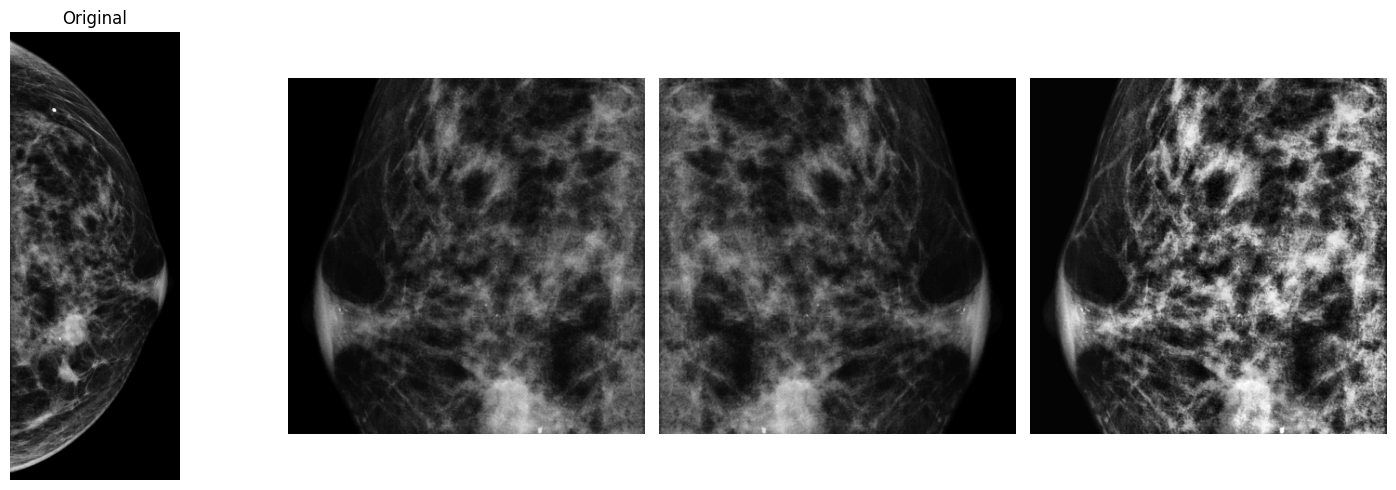
\includegraphics[width=0.8\linewidth]{reports//assets/augmentations.png}
\caption[Aumentos de imagen]{Ejemplo de aumentos de imagen.}
\label{fig:augmentations}
\end{figure}


\textbf{Uso de la Pérdida de Entropía Cruzada Ponderada}

La función de pérdida de entropía cruzada es una función que mide la diferencia entre las distribuciones de clases predichas y reales. La versión ponderada aplica un factor de escala (típicamente el inverso de las frecuencias de clase) para abordar eficazmente el desequilibrio de clases o enfatizar ciertas clases durante el entrenamiento del modelo. Matemáticamente, puede expresarse como:

\begin{equation}
J_{\text{WCE}} = -\frac{1}{M} \sum_{m=1}^{M} \sum_{k=1}^{K} w_k \; y_{m,k} \; \log\left( h_\theta(x_m, k) \right)
\end{equation}

Donde: $J_{\text{WCE}}$~: pérdida de entropía cruzada ponderada, $M$~: número de muestras en el batch, $K$~: número de clases, $w_k$~: peso para la clase~$k$, $y_{m,k}$~: indicador (1 si la muestra~$m$ pertenece a la clase~$k$, si no~0), y $h_\theta(x_m, k)$~: probabilidad predicha para la clase~$k$ (salida softmax).

Esta función de pérdida puede ayudar a mejorar significativamente el rendimiento del modelo en conjuntos de datos desbalanceados.

\textbf{Uso de Weighted Random Sampler}

El muestreo aleatorio ponderado (Weighted Random Sampler) es otra técnica para mitigar el desequilibrio de clases. En este enfoque, las probabilidades de muestreo se asignan en función de la frecuencia inversa de cada clase, otorgando a las muestras de clases minoritarias una mayor probabilidad de ser seleccionadas durante el entrenamiento por lotes en comparación con las muestras de clases mayoritarias. Esto resulta especialmente útil en conjuntos de datos como CMMD2, donde una clase, como Luminal B, domina y tiene significativamente más muestras que las demás.

Sin embargo, una limitación clave es que el muestreo aleatorio ponderado no debe combinarse con la pérdida de entropía cruzada ponderada, ya que ambas técnicas abordan el desequilibrio de clases y su uso conjunto puede llevar a una sobrecompensación, introduciendo potencialmente sesgos durante el entrenamiento. Por esta razón, el muestreo aleatorio ponderado se implementa como una modalidad experimental separada. La Figura~\ref{fig:batch_sampling} muestra la distribución típica de clases dentro de un lote (batch size 32), mientras que la Figura~\ref{fig:batch_sampling_weighted} ilustra la distribución tras aplicar el Weighted Random Sampler.

\begin{figure}[h!]
\centering
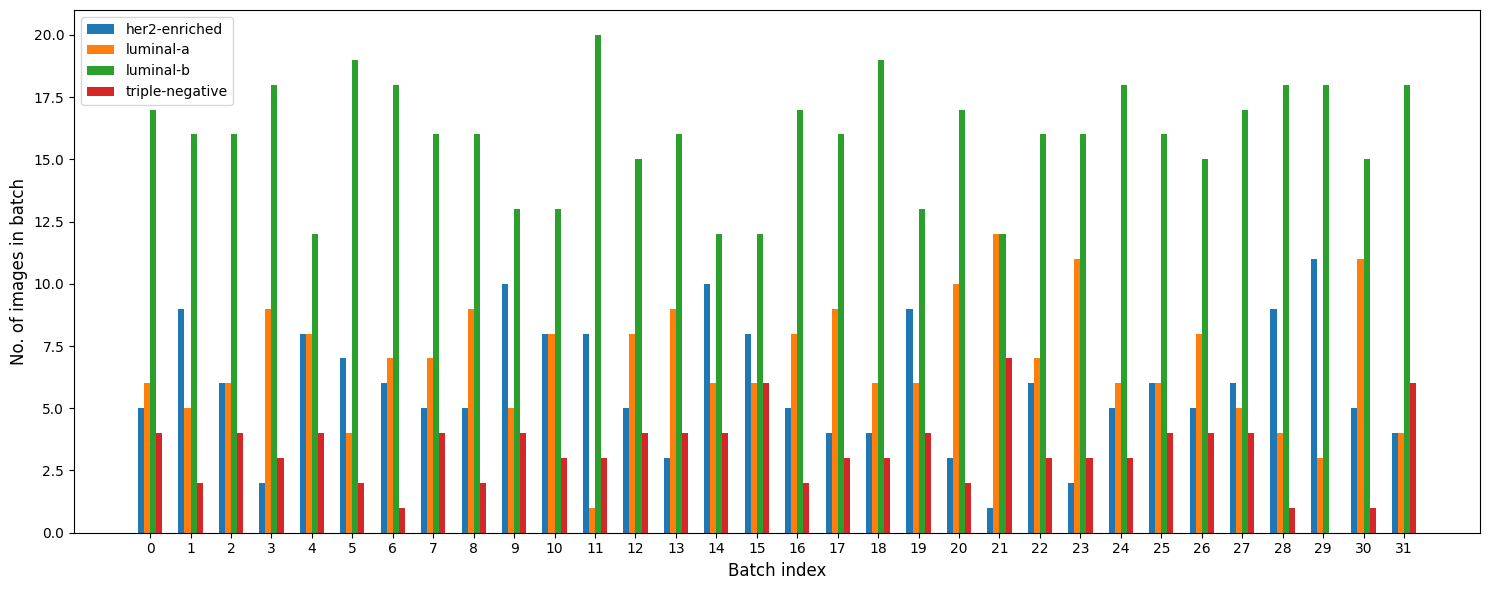
\includegraphics[width=.8\linewidth]{reports//assets/sampler.png}
\caption[Batch Sampling (Default)]{Distribución de clases dentro de un lote típico (batch size = 32) durante una época de entrenamiento usando muestreo por defecto. El número promedio de imágenes por lote para cada clase es: HER2: 6.03, LumA: 6.72, LumB: 15.75 y TN: 3.50.}
\label{fig:batch_sampling}
\end{figure}

\begin{figure}[ht!]
\centering
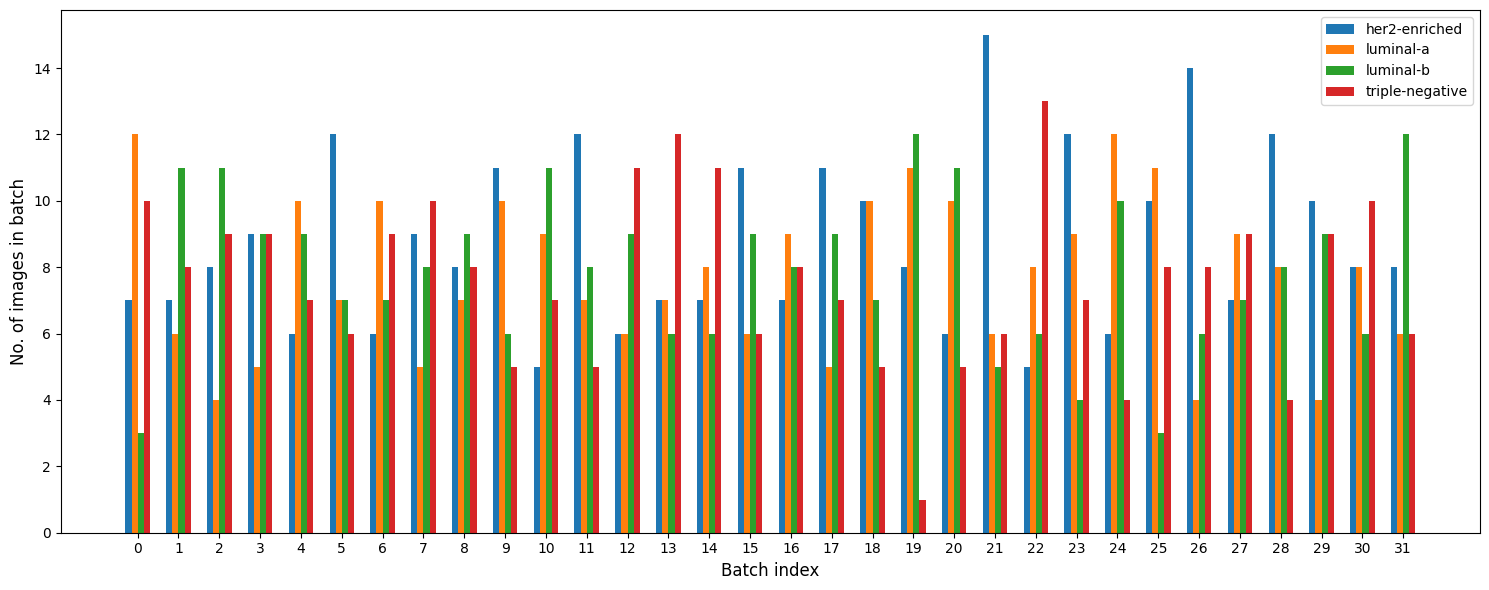
\includegraphics[width=0.8\linewidth]{reports//assets/sampler2.png}
\caption[Batch Sampling (Weighted)]{Distribución de clases dentro de un lote (batch size = 32) tras aplicar muestreo aleatorio ponderado. El número promedio de imágenes por lote para cada clase es: HER2: 8.25, LumA: 7.88, LumB: 7.28 y TN: 8.59.}
\label{fig:batch_sampling_weighted}
\end{figure}

\subsection{Prueba Estadística}

Tras completar los experimentos, estos deben evaluarse estadísticamente. En estudios de esta naturaleza, es práctica común aplicar métodos estadísticos para determinar si las diferencias observadas en el rendimiento de los modelos son significativas o podrían haberse producido por azar. La metodología habitual implica un análisis estadístico en dos pasos. Para este estudio, primero se realizó una prueba de Friedman para evaluar las diferencias generales entre modelos, seguida de pruebas de rangos con signo de Wilcoxon para comparaciones por pares entre modelos \cite{demsar_statistical_2006}.

\subsubsection{Prueba de Friedman}

La prueba de Friedman es una prueba estadística simple y no paramétrica\footnote{Los métodos no paramétricos son técnicas estadísticas que no asumen una distribución específica para los datos, lo que las hace adecuadas para datos no normales u ordinales.} utilizada para comparar tres o más grupos relacionados. La hipótesis nula es que todos los modelos tienen un rendimiento igual, es decir, no existen diferencias significativas en sus medianas de rendimiento a lo largo de mediciones repetidas \cite{demsar_statistical_2006}. Para realizar la prueba, el rendimiento de cada modelo (por ejemplo, AUC) se ordena dentro de cada unidad experimental (como cada combinación de fold, semilla y modalidad). Luego, la estadística de la prueba se calcula como:

\begin{equation}
\chi^2_F = \frac{12}{nk(k+1)} \sum_{j=1}^{k} R_j^2 - 3n(k+1)
\end{equation}

\noindent
Donde $n$ es el número de unidades experimentales, $k$ es el número de modelos comparados, y $R_j$ es la suma de rangos para el modelo $j$. Esta estadística sigue una distribución chi-cuadrado con $k-1$ grados de libertad. Si el valor p resultante\footnote{Una medida de cuán probables son los resultados observados si no existiera una diferencia o efecto real.} es menor que 0.05, se puede rechazar la hipótesis nula.

\subsubsection{Prueba de Rangos con Signo de Wilcoxon}

La prueba de rangos con signo de Wilcoxon es una prueba no paramétrica utilizada para determinar si existe una diferencia estadísticamente significativa entre dos conjuntos de valores emparejados o relacionados. Consiste en ordenar las diferencias absolutas entre cada par, y luego comparar las sumas de los rangos positivos y negativos para evaluar si las diferencias observadas son probablemente debidas al azar o reflejan un efecto real \cite{demsar_statistical_2006}. La estadística de la prueba se define como:

\begin{equation}
W = \min \left( W^+,\, W^- \right)
\end{equation}

Donde $W^+$ es la suma de los rangos para las diferencias positivas, y $W^-$ es la suma de los rangos para las diferencias negativas.

\chapter{Resultados y Discusión}

Este capítulo presenta los principales hallazgos del estudio, incluyendo la evaluación del rendimiento de los modelos propuestos y las modalidades de entrenamiento para la subtipificación molecular del cáncer de mama utilizando imágenes mamográficas. Los resultados se analizan utilizando las métricas de evaluación y los métodos estadísticos descritos en los capítulos anteriores. Los análisis comparativos resaltan las fortalezas y limitaciones de cada enfoque, y se discuten las implicaciones de estos hallazgos en el contexto de la investigación actual.

\section{Resultados de los Experimentos}

Se realizaron un total de 144 experimentos para recopilar las métricas de validación cruzada. Como se definió anteriormente, cada modelo se entrenó utilizando validación cruzada de 3 folds, registrando las métricas de validación para cada fold a lo largo de 3 particiones distintas de entrenamiento y prueba (semillas 0, 21 y 42) y 4 modalidades diferentes. Para asegurar la fiabilidad de los resultados, cada experimento utilizó la misma semilla para la partición K-Fold, garantizando particiones de datos consistentes en todas las ejecuciones. El conjunto completo de resultados se presenta en la Tabla~\ref{tab:complete_metrics}, mientras que los resultados promediados por semilla se muestran en las Tablas~\ref{tab:avg_metrics_seed_0}, \ref{tab:avg_metrics_seed_21} y \ref{tab:avg_metrics_seed_42}. Para ofrecer una visión general de las métricas de validación obtenidas mediante validación cruzada K-Fold para cada semilla, la Tabla~\ref{tab:per_seed_metrics_avg} presenta los valores promediados.


\begin{scriptsize}
\begin{longtable}{@{}l l p{0.6cm} p{1.5cm} p{1.5cm} p{1.5cm} p{1.5cm} p{1.5cm}@{}}
\caption[Métricas de validación promedio por semilla]{Métricas de validación promedio por semilla obtenidas tras validación cruzada de 3 folds en 3 particiones diferentes de entrenamiento y prueba.}
\label{tab:per_seed_metrics_avg}\\
\toprule
\textbf{Modelo} & \textbf{Muestreo} & \textbf{Aum.} &
\textbf{B.\ Acc.} & \textbf{AUC} & \textbf{F1} &
\textbf{Prec.} & \textbf{C.\ Kappa} \\
\midrule
\endfirsthead

\toprule
\textbf{Modelo} & \textbf{Muestreo} & \textbf{Aum.} &
\textbf{B.\ Acc.} & \textbf{AUC} & \textbf{F1} &
\textbf{Prec.} & \textbf{C.\ Kappa} \\
\midrule
\endhead

\midrule
\multicolumn{8}{r}{\textit{Continua en la siguiente página.}}\\
\midrule
\endfoot

\bottomrule
\endlastfoot
ResNet101 & Weighted    & No  & 0.2977 $\pm$ 0.032  & 0.5649 $\pm$ 0.0307 & 0.2788 $\pm$ 0.0345 & 0.2842 $\pm$ 0.0356 & 0.0734 $\pm$ 0.0409 \\
ResNet101 & Weighted    & Yes & 0.3133 $\pm$ 0.0158 & 0.5692 $\pm$ 0.0215 & 0.2941 $\pm$ 0.0213 & 0.3037 $\pm$ 0.0218 & 0.0931 $\pm$ 0.0250 \\
ResNet101 & Oversampled & No  & 0.2971 $\pm$ 0.0259 & 0.5619 $\pm$ 0.0294 & 0.2699 $\pm$ 0.0333 & 0.3049 $\pm$ 0.0295 & 0.0677 $\pm$ 0.0384 \\
ResNet101 & Oversampled & Yes & 0.3002 $\pm$ 0.0298 & 0.5681 $\pm$ 0.0241 & 0.2530 $\pm$ 0.0489 & 0.3229 $\pm$ 0.0777 & 0.0647 $\pm$ 0.0421 \\
ViT       & Weighted    & No  & 0.3319 $\pm$ 0.0439 & 0.5852 $\pm$ 0.0202 & 0.3002 $\pm$ 0.0450 & 0.3158 $\pm$ 0.0457 & 0.0888 $\pm$ 0.0466 \\
\textbf{ViT} & \textbf{Weighted} & \textbf{Yes} &
\textbf{0.3397 $\pm$ 0.0255} & \textbf{0.5864 $\pm$ 0.0202} &
\textbf{0.3062 $\pm$ 0.0467} & \textbf{0.3313 $\pm$ 0.0338} &
\textbf{0.1066 $\pm$ 0.0436} \\
ViT       & Oversampled & No  & 0.3134 $\pm$ 0.0378 & 0.5821 $\pm$ 0.0235 & 0.2816 $\pm$ 0.0273 & 0.3178 $\pm$ 0.0304 & 0.0719 $\pm$ 0.0367 \\
ViT       & Oversampled & Yes & 0.3214 $\pm$ 0.0293 & 0.5820 $\pm$ 0.0172 & 0.2923 $\pm$ 0.0406 & 0.3082 $\pm$ 0.0347 & 0.0867 $\pm$ 0.0362 \\
Swin      & Weighted    & No  & 0.3212 $\pm$ 0.0292 & 0.5819 $\pm$ 0.0193 & 0.2836 $\pm$ 0.0355 & 0.3083 $\pm$ 0.0207 & 0.0814 $\pm$ 0.0334 \\
Swin      & Weighted    & Yes & 0.3170 $\pm$ 0.0232 & 0.5825 $\pm$ 0.0169 & 0.2811 $\pm$ 0.0327 & 0.3051 $\pm$ 0.0254 & 0.0812 $\pm$ 0.0288 \\
Swin      & Oversampled & No  & 0.3152 $\pm$ 0.0183 & 0.5775 $\pm$ 0.0161 & 0.2838 $\pm$ 0.0325 & 0.3132 $\pm$ 0.0157 & 0.0790 $\pm$ 0.0180 \\
Swin      & Oversampled & Yes & 0.3143 $\pm$ 0.0211 & 0.5820 $\pm$ 0.0208 & 0.2806 $\pm$ 0.0391 & 0.3147 $\pm$ 0.0272 & 0.0812 $\pm$ 0.0317 \\
MaxVit    & Weighted    & No  & 0.3155 $\pm$ 0.0086 & 0.5776 $\pm$ 0.0171 & 0.3010 $\pm$ 0.0103 & 0.3098 $\pm$ 0.0116 & 0.0618 $\pm$ 0.0210 \\
MaxVit    & Weighted    & Yes & 0.3140 $\pm$ 0.0261 & 0.5836 $\pm$ 0.0255 & 0.2875 $\pm$ 0.0343 & 0.3119 $\pm$ 0.0332 & 0.0686 $\pm$ 0.0371 \\
MaxVit    & Oversampled & No  & 0.3157 $\pm$ 0.0270 & 0.5799 $\pm$ 0.0202 & 0.2886 $\pm$ 0.0240 & 0.2969 $\pm$ 0.0212 & 0.0649 $\pm$ 0.0322 \\
MaxVit    & Oversampled & Yes & 0.3107 $\pm$ 0.0355 & 0.5805 $\pm$ 0.0248 & 0.2896 $\pm$ 0.0297 & 0.3096 $\pm$ 0.0283 & 0.0637 $\pm$ 0.0438 \\
\end{longtable}
\end{scriptsize}


A partir de estos resultados promediados, se destaca que el modelo con mejor desempeño es ViT, que alcanza las métricas de validación más altas, especialmente en la modalidad que utiliza Pérdida de Entropía Cruzada Ponderada y Aumento de Datos. Aunque los resultados son modestos y tanto el entrenamiento como la validación se realizaron utilizando únicamente la cabeza del clasificador, esto proporciona una indicación inicial del rendimiento general del modelo.

Al centrarse exclusivamente en la métrica AUC, los modelos y modalidades con mejor desempeño se presentan en la Tabla \ref{tab:best_auc_modalities_validation}.

\begin{table}[h!]
  \centering
\caption[Mejores puntuaciones de AUC de validación por modelo y modalidad.]{Mejores puntuaciones de AUC de validación por modelo y modalidad.}
  \label{tab:best_auc_modalities_validation}
  \begin{tabular}{l l c c}
    \toprule
    \textbf{Model} & \textbf{Sampling} & \textbf{Augmentation} & \textbf{AUC} \\ 
    \midrule
    ViT & Weighted & Yes & 0.5864  $\pm$ 0.0202   \\
    MaxVit  & Weighted & Yes  & 0.5836 $\pm$  0.0255 \\
    Swin    & Weighted & Yes  & 0.5825 $\pm$  0.0169 \\
    ResNet-101    & Oversample & No & 0.5681 $\pm$  0.0241 \\
    \bottomrule
  \end{tabular}
\end{table}


Aunque estas puntuaciones son bastante bajas, esto es comprensible dada la dificultad inherente de la clasificación multiclase y la alta heterogeneidad de los subtipos moleculares. No obstante, basándonos únicamente en estas observaciones, podemos sospechar que nuestra hipótesis de estudio (que los modelos basados en transformers generalizan algo mejor que nuestra línea base de CNN) se ve respaldada. Las diferencias de rendimiento a lo largo de los tres folds, especialmente en métricas como AUC y F1-score, sugieren que los modelos basados en transformers pueden estar capturando patrones más complejos al clasificar subtipos moleculares en comparación con la arquitectura ResNet-101.

Para asegurar que estos hallazgos no se deban al azar o a la variabilidad experimental, se realizó una prueba de significancia estadística. En concreto, se aplicó una prueba de Friedman a todas las métricas de validación recolectadas (Tabla \ref{tab:complete_metrics}). Esta prueba determina si existen diferencias estadísticamente significativas entre los experimentos para cada métrica, considerándose significativo un valor p menor a 0.05. La Tabla \ref{tab:friedman_test_results} resume estos resultados.

\begin{table}[h!]
  \centering
\caption[Resumen de estadísticas y valores p de la prueba de Friedman para todas las métricas de evaluación.]{Estadísticas de la prueba de Friedman y valores p correspondientes para las diferentes métricas de evaluación que comparan el rendimiento de modelos y modalidades en el conjunto de validación. Los resultados estadísticamente significativos ($p < 0.05$) se resaltan en negrita.}
  \label{tab:friedman_test_results}
  \begin{tabular}{l l c c}
    \toprule
    \textbf{Metrica} & \textbf{Estadístico de Friedman} & \textbf{p-value} \\
    \midrule
    Balanced Accuracy & 8.53 & \textbf{0.03}  \\
    AUC  & 15.36  &  \textbf{0.001 }\\
    Macro F1-Score    &  5.36  & 0.15 \\
    Macro Precision & 2.23 &  0.52 \\
    Cohen-Kappa & 4.89 & 0.18 \\
    \bottomrule
  \end{tabular}
\end{table}

Estos resultados muestran que los valores p para Precisión Balanceada y AUC están por debajo del umbral de significancia de 0.05, lo que indica diferencias estadísticamente significativas entre los modelos o modalidades para estas métricas. En otras palabras, al menos un modelo o modalidad tiene un rendimiento diferente al de los demás en términos de Precisión Balanceada y AUC. Para las métricas restantes, los valores p son superiores a 0.05, por lo que no hay suficiente evidencia para concluir que existan diferencias significativas entre los grupos. Esto sugiere que los modelos tienen un rendimiento similar respecto a estas métricas, o que las diferencias observadas probablemente se deben a la variabilidad aleatoria.

Con base en estos hallazgos, se realizó una prueba de rangos con signo de Wilcoxon para identificar qué modelos tienen un rendimiento significativamente mejor que otros en términos de Precisión Balanceada y AUC.

\begin{table}[h!]
  \centering
    \caption[Valores p de la prueba de rangos con signo de Wilcoxon para cada par de modelos.]{Valores p de la prueba de rangos con signo de Wilcoxon para cada par de modelos, tanto para Precisión Balanceada como para AUC. Los resultados estadísticamente significativos ($p < 0.05$) se resaltan en negrita.}
  \label{tab:wilcoxon_pvalues}
  \begin{tabular}{@{}lcc@{}}
    \toprule
    \textbf{Model Pair} & \textbf{Balanced Accuracy (p-value)} & \textbf{AUC (p-value)} \\
    \midrule
    ResNet101 vs. ViT      & \textbf{0.004} & \textbf{0.008} \\
    ResNet101 vs. Swin     & \textbf{0.02} & \textbf{0.01} \\
    ResNet101 vs. MaxVit   & \textbf{0.03} & \textbf{0.007} \\
    ViT vs. Swin           & 0.101 & 0.809 \\
    ViT vs. MaxVit         & 0.111 & 0.508 \\
    Swin vs. MaxVit        & 0.658 & 0.882 \\
    \bottomrule
  \end{tabular}
\end{table}

Como se muestra en la Tabla~\ref{tab:wilcoxon_pvalues}, todos los modelos basados en transformers presentan diferencias estadísticamente significativas en comparación con ResNet-101 tanto en Precisión Balanceada como en AUC. Es destacable que ViT y MaxVit muestran los valores p más bajos para AUC al compararse con ResNet-101, lo que indica diferencias particularmente marcadas. Estos resultados respaldan los hallazgos presentados en la Tabla~\ref{tab:best_auc_modalities_validation}. Por lo tanto, tenemos evidencia significativa para concluir que los modelos basados en transformers superan a ResNet-101 respecto a estas métricas. Para los pares de modelos restantes, la prueba de rangos con signo de Wilcoxon no reveló diferencias estadísticamente significativas, lo que sugiere que los modelos basados en transformers tienen un rendimiento comparable entre sí en estas métricas. En conjunto, estos hallazgos brindan un sólido respaldo a nuestra hipótesis de que los modelos basados en transformers logran un rendimiento superior en comparación con las CNN para esta tarea.

\section{Ajuste fino y evaluación en el conjunto de prueba}

Una vez establecidas las diferencias estadísticas, se realizó una fase de ajuste fino (fine-tuning). Las modalidades con mejores resultados promediados, como se muestra en la Tabla~\ref{tab:best_auc_modalities_validation}, fueron seleccionadas para esta fase a lo largo de las tres particiones de entrenamiento y prueba. En esta etapa, se utilizó todo el conjunto de entrenamiento para el entrenamiento del modelo, y posteriormente se realizó la evaluación en el conjunto de prueba correspondiente.

El proceso de ajuste fino se llevó a cabo utilizando los mismos hiperparámetros listados en la Tabla~\ref{tab:hyperparams}, excepto por la tasa de aprendizaje, que se estableció en un valor diez veces menor. Además, el entrenamiento se realizó en dos etapas: primero, se entrenó la cabeza del clasificador durante 10 épocas; luego, se realizó el ajuste fino durante 5 épocas con todas las capas del backbone descongeladas, para evitar el sobreajuste.

Los resultados completos pueden consultarse en la Tabla \ref{tab:test_set_results}, pero la Tabla \ref{tab:test_set_results_avg} resume el promedio por semilla.

\begin{scriptsize}
\begin{longtable}{@{}l c c c c c@{}}
\caption[Resultados promedios en el conjunto de prueba]{Promedio de resultados en el conjunto de prueba tras el ajuste fino en tres particiones diferentes de entrenamiento y prueba.}
\label{tab:test_set_results_avg} \\
\toprule
\textbf{Model} & \textbf{B. Acc.} & \textbf{AUC} & \textbf{F1} & \textbf{Prec.}  & \textbf{C.\ Kappa}\\
\midrule
\endfirsthead

\toprule
\textbf{Model} & \textbf{B. Acc.} & \textbf{AUC} & \textbf{F1} & \textbf{Prec.} & \textbf{C.\ Kappa}\\
\midrule
\endhead

\midrule
\multicolumn{6}{r}{\textit{Continued on next page}}\\
\midrule
\endfoot

\bottomrule
\endlastfoot
     \textbf{ViT} & \textbf{0.385 $\pm$ 0.042} & \textbf{0.635  $\pm$ 0.016} & \textbf{0.354  $\pm$ 0.049} & \textbf{0.362  $\pm$ 0.039} & \textbf{0.159  $\pm$ 0.063}  \\
     MaxVit & 0.341 $\pm$ 0.016 & 0.605 $\pm$  0.019 & 0.325 $\pm$  0.012 & 0.336 $\pm$  0.011 & 0.12 $\pm$  0.021 \\
    Swin & 0.358 $\pm$  0.033 & 0.619 $\pm$  0.008 & 0.319 $\pm$  0.041 & 0.339 $\pm$  0.051 & 0.118 $\pm$  0.04 \\
    ResNet-101 & 0.322 $\pm$  0.062 & 0.563 $\pm$  0.03 & 0.285 $\pm$  0.07 & 0.337 $\pm$  0.112 & 0.095 $\pm$  0.078 \\
\end{longtable}
\end{scriptsize}


Como se muestra en los resultados promedios del conjunto de prueba, los modelos basados en transformers superan a ResNet-101 en casi todas las métricas, especialmente en la puntuación AUC. El modelo con mejor desempeño fue ViT, que alcanzó los valores más altos en todos los experimentos. Esto sugiere que el mecanismo de atención global en ViT puede desempeñar un papel significativo en esta tarea de clasificación, en contraste con las operaciones locales del modelo ResNet-101.

Sin embargo, es importante señalar que estas métricas siguen siendo bastante bajas y están por debajo del umbral clínicamente aceptado. No obstante, los resultados resaltan el potencial de los modelos basados en transformers o de los mecanismos de atención en la clasificación de subtipos moleculares de cáncer de mama.

La Figura \ref{fig:mean_auc_images} muestra las curvas promedio de AUC de los modelos en el conjunto de prueba y revela algunos detalles interesantes. A partir de estas curvas, se observa que la clase más fácil de clasificar es HER2-Enriched; en todos los casos, es la clase con el rendimiento más destacado en todos los modelos. Otro patrón interesante es que la clase Triple Negativo, que es la clase minoritaria en el conjunto de datos y la más difícil de clasificar debido a su alta heterogeneidad \cite{sinn_triple-negative_2023}, es más clasificable por los modelos basados en transformers que por ResNet-101. Este hallazgo es especialmente valioso, ya que indica que, a pesar de la significativa heterogeneidad de la clase, los mecanismos de atención pueden aprovechar patrones útiles para su clasificación.

\begin{figure}[h!]
    \centering
    \begin{subfigure}[t]{0.48\textwidth}
        \centering
        \includegraphics[width=\textwidth]{reports/assets/MEAN_AUC_Vit.png}
        \caption{ViT}
        \label{fig:mean_auc_vit}
    \end{subfigure}
    \begin{subfigure}[t]{0.48\textwidth}
        \centering
        \includegraphics[width=\textwidth]{reports/assets/MEAN_AUC_ResNet.png}
        \caption{ResNet-101}
        \label{fig:mean_auc_resnet}
    \end{subfigure}
    \vspace{0.5cm}
    \begin{subfigure}[t]{0.48\textwidth}
        \centering
        \includegraphics[width=\textwidth]{reports/assets/MEAN_AUC_MaxVit.png}
        \caption{MaxVit}
        \label{fig:mean_auc_maxvit}
    \end{subfigure}
    \begin{subfigure}[t]{0.48\textwidth}
        \centering
        \includegraphics[width=\textwidth]{reports/assets/MEAN_AUC_Swin.png}
        \caption{Swin}
        \label{fig:mean_auc_swin}
    \end{subfigure}
    \caption[Curvas promedio de AUC]{Curvas promedio de AUC para cada modelo (ViT, ResNet, MaxVit y Swin). Cada curva representa el AUC promedio a través de las tres particiones de entrenamiento y prueba.}
    \label{fig:mean_auc_images}
\end{figure}

Ahora nos centramos en los modelos ViT y ResNet con mejor desempeño, ambos derivados de la partición Seed 42 de entrenamiento y prueba (véase la Tabla \ref{tab:test_set_results}). El primero alcanza un AUC del 65.09\% y el mejor ResNet alcanza un AUC del 58.84\%. La Figura \ref{fig:cm_vit_resnet} muestra las matrices de confusión de estos modelos.

\begin{figure}[h!]
    \centering
    \begin{subfigure}[t]{0.48\textwidth}
        \centering
        \includegraphics[width=\textwidth]{reports/assets/CM-42-ViT.png}
        \caption{}
        \label{fig:cm_vit}
    \end{subfigure}
    \begin{subfigure}[t]{0.48\textwidth}
        \centering
        \includegraphics[width=\textwidth]{reports/assets/CM-42-ResNet.png}
        \caption{}
        \label{fig:cm_resnet}
    \end{subfigure}
    \caption[Matrices de confusión Mejor ViT vs. Mejor ResNet]{Matrices de confusión del mejor ViT (a) y del mejor ResNet-101 (b). Clases: 0 = HER2-enriquecido, 1 = Luminal A, 2 = Luminal B, 3 = TN.}
    \label{fig:cm_vit_resnet}
\end{figure}

Las matrices de confusión demuestran que el modelo ViT supera de manera consistente al modelo ResNet-101, lo que corrobora nuestros hallazgos previos. Ambos modelos muestran un excelente rendimiento para el subtipo HER2-Enriched, alcanzando una alta precisión de clasificación (33/50 predicciones correctas para ViT y 32/50 para ResNet-101). Este desempeño confirma nuestra observación anterior de que HER2-Enriched es el subtipo molecular más distinguible en todos los modelos evaluados. Para la clasificación de Luminal A, las predicciones muestran diferencias notables: ViT clasificó correctamente 19/56 casos, mientras que ResNet-101 logró 22/56 clasificaciones correctas. Sin embargo, ViT demuestra una menor tasa de errores de clasificación cruzada, especialmente con el subtipo TN. ViT también muestra un rendimiento superior en la clasificación de casos Luminal B, logrando 58/136 clasificaciones correctas frente a 51/136 de ResNet-101, lo que evidencia mejores patrones de discriminación. Finalmente, aunque la clase TN es la más difícil de clasificar, ViT demuestra que puede captar mejor las características complejas de este subtipo.

Estos resultados coinciden con la literatura reciente, donde los modelos Vision Transformer (ViT) han mostrado un rendimiento superior en la clasificación de cáncer de mama respecto a arquitecturas CNN convencionales como ResNet, alcanzando mayores valores de precisión, recall y F1-score, y destacando la capacidad de los mecanismos de atención para capturar tanto información global como local en imágenes médicas. Sin embargo, algunos estudios señalan que, dependiendo de la estrategia de entrenamiento y el conjunto de datos, ResNet101 puede acercarse al rendimiento de ViT en ciertos escenarios específicos.

Adicionalmente, se presenta la representación t-SNE\footnote{t-Distributed Stochastic Neighbor Embedding es un método estadístico potente para visualizar datos de alta dimensión reduciéndolos a un mapa bidimensional o tridimensional.} para la clasificación de cada modelo, con el fin de evaluar la capacidad de los modelos para agrupar las diferentes clases de subtipos moleculares (Figura \ref{fig:tsne_vit_resnet}).

\begin{figure}[h!]
    \centering
    \begin{subfigure}[t]{0.48\textwidth}
        \centering
        \includegraphics[width=\textwidth]{reports/assets/TSNE-VIT.png}
        \caption{ViT}
        \label{fig:tsne_vit}
    \end{subfigure}
    \begin{subfigure}[t]{0.48\textwidth}
        \centering
        \includegraphics[width=\textwidth]{reports/assets/TSNE-ResNet.png}
        \caption{ResNet-101}
        \label{fig:tsne_resnet}
    \end{subfigure}
    \caption[Visualizaciones t-SNE Mejor ViT vs. Mejor ResNet-101]{Visualizaciones t-SNE de las representaciones de características aprendidas por el mejor ViT (a) y el mejor ResNet-101 (b).}
    \label{fig:tsne_vit_resnet}
\end{figure}

Estas visualizaciones demuestran que el modelo ViT logra una organización superior de las características en comparación con ResNet-101, con patrones de agrupamiento más definidos, especialmente visibles en las regiones superiores donde los casos HER2-enriquecido forman agrupaciones más compactas. Aunque ambos modelos presentan solapamiento entre Luminal A y Luminal B, ViT muestra una mejor separación de los subtipos moleculares y una menor mezcla de casos Triple Negativo con otras clases. Si bien esta evidencia visual no es perfecta, respalda la idea de que los Vision Transformers capturan mejor las características discriminativas mamográficas para la subtipificación molecular que las arquitecturas CNN tradicionales.

\subsection{Breve análisis de explicabilidad}

El análisis de explicabilidad proporciona información crítica sobre los procesos de toma de decisiones del modelo y mejora la confianza clínica. Se compararon el modelo ViT con mejor desempeño y ResNet-101 específicamente para la clasificación HER2-Enriched, dada la capacidad demostrada del modelo ViT para distinguir este subtipo molecular, como se estableció en secciones previas.

Para el modelo ResNet-101 se empleó Captum \cite{noauthor_captum_nodate, noauthor_161002391_nodate} con GRAD-Cam, y para ViT se utilizó el algoritmo ViT-ReciproCam \cite{byun_vit-reciprocam_2023}.

\begin{figure}[h!]
\centering
\begin{subfigure}[c]{0.48\textwidth}
\centering
\includegraphics[width=\textwidth]{reports//assets/D2-0138_MLO-R_Resnet.png}
\caption{}
\label{fig:mlo_grad}
\end{subfigure}
\begin{subfigure}[c]{0.48\textwidth}
\centering
\includegraphics[width=\textwidth]{reports//assets/D2-0138_MLO-R.png}
\caption{}
\label{fig:mlo_reci}
\end{subfigure}
\caption[GradCAM vs. ViT-ReciproCAM (vista MLO)]{GradCAM (a) vs. ViT-ReciproCAM (b) en una mamografía MLO.}
\label{fig:grad_vs_vit}
\end{figure}

En la Figura \ref{fig:grad_vs_vit}, se comparan las salidas de explicabilidad de ambos métodos para una mamografía MLO HER2-Enriched del conjunto de prueba. Grad-CAM de ResNet-101 resalta las atribuciones de píxeles que contribuyen a la predicción mediante el análisis de gradientes, mientras que ViT-ReciproCAM identifica regiones salientes enmascarando iterativamente tokens en el espacio de características del transformer y midiendo el impacto en la predicción.

Ambos modelos detectan con éxito la masa presente en la imagen; sin embargo, sus patrones de atribución difieren notablemente. La salida de Grad-CAM resalta regiones específicas y localizadas con límites discretos, mientras que el mapa de atribución de ViT-ReciproCAM muestra una cobertura más difusa con regiones de importancia más amplias. Esta diferencia refleja la tendencia del Vision Transformer a capturar patrones globales y distribuidos en toda la imagen, en contraste con el enfoque localizado y basado en parches de la CNN.

Utilizando la máscara de segmentación MLO de TOMPEI-CMMD\cite{kashiwada_tompei-cmmd_2025}, se muestra una comparación entre ambos modelos en la Figura \ref{fig:grad_vs_vit_two}. Los resultados indican que el modelo ViT se enfoca de manera más precisa en la región de la masa para la clasificación, en comparación con ResNet-101, que muestra una localización menos precisa en su mapa de atribución.



\begin{figure}[h!]
    \centering
    \begin{subfigure}[c]{0.30\textwidth}
        \centering
        \includegraphics[width=\textwidth]{reports//assets/path.png}
        \caption{}
        \label{fig:tompei_patch}
    \end{subfigure}
    \begin{subfigure}[c]{0.30\textwidth}
        \centering
        \includegraphics[width=\textwidth]{reports//assets/gcam.png}
        \caption{}
        \label{fig:mlo_grad_2}
    \end{subfigure}
      \begin{subfigure}[c]{0.30\textwidth}
        \centering
        \includegraphics[width=\textwidth]{reports//assets/recipro.png}
        \caption{}
        \label{fig:mlo_recipro_2}
    \end{subfigure}
    \caption[GradCAM vs. ViT-Recipro con Segmentación TOMPEI]{Mamografía con segmentación de masa (a), Grad-CAM (b), ViT-ReciproCAM (c)}
    \label{fig:grad_vs_vit_two}
\end{figure}


Esto se corrobora aún más en la Figura \ref{fig:grad_vs_vit_cc}, donde se analiza la vista CC de este mismo paciente. Aquí se observa nuevamente que ViT considera una zona más amplia de la mamografía, abarcando una región más extensa que los límites reales de la masa, mientras que el Grad-CAM de ResNet-101 proporciona atribuciones espacialmente más restringidas que corresponden estrechamente a las regiones de tejido denso visibles en la imagen original.



\begin{figure}[h!]
    \centering
    \begin{subfigure}[c]{0.48\textwidth}
        \centering
        \includegraphics[width=\textwidth]{reports//assets/D2-0138_CC-R_Resnet.png}
        \caption{}
        \label{fig:cc_cam}
    \end{subfigure}
    \begin{subfigure}[c]{0.48\textwidth}
        \centering
        \includegraphics[width=\textwidth]{reports//assets/D2-0138_CC-R.png}
        \caption{}
        \label{fig:cc_reci}
    \end{subfigure}
     \caption[GradCAM vs. ViT-ReciproCAM (vista CC)]{GradCAM (a) vs. ViT-ReciproCAM (b) en una mamografía CC.}
    \label{fig:grad_vs_vit_cc}
\end{figure}

En resumen, la atención global de ViT parece ser un enfoque más eficaz para capturar patrones distribuidos y ricos en contexto a lo largo de toda la mamografía, permitiendo que el modelo considere regiones más amplias que pueden ser relevantes para una clasificación precisa.



\subsection{Comparación de Rendimiento con la Literatura Reciente}

Como se indicó previamente, investigaciones recientes han aportado información relevante sobre este mismo problema. Comparar nuestros resultados es un paso crucial para validar nuestros hallazgos. Por esta razón, los trabajos realizados por Mota et al.\ \cite{mota_breast_2024} y Rabah et al.\ \cite{ben_rabah_multimodal_2025} se utilizaron como referencias en este estudio. Es importante, sin embargo, dejar claro que existen diferencias en los entornos experimentales y en los parámetros de estudio entre los distintos trabajos. La Tabla \ref{tab:studies_comparison} resume sus resultados y configuraciones, y los compara con los obtenidos en nuestro estudio.

\begin{scriptsize}
\begin{longtable}{@{}l l l l l l l l l l@{}}
\caption[Comparación con estudios relacionados]{Comparación con estudios relacionados sobre la subtipificación molecular del cáncer de mama utilizando diferentes conjuntos de datos, arquitecturas de modelos y configuraciones experimentales.}
\label{tab:studies_comparison} \\
\toprule
\textbf{Estudio} & \textbf{Dataset} & \textbf{Clases} & \textbf{Pacientes} & \textbf{Imagenes} &  \textbf{Tamaño} & \textbf{Modelo}  & \textbf{ROI} & \textbf{Acc.}  & \textbf{AUC}\\
\midrule
\endfirsthead

\toprule
\textbf{Estudio} & \textbf{Dataset} & \textbf{Clases} & \textbf{Pacientes} & \textbf{Imagenes} &  \textbf{Tamaño} & \textbf{Modelo}  & \textbf{ROI} & \textbf{Acc.}  & \textbf{AUC}\\
\midrule
\endhead

\midrule
\multicolumn{10}{r}{\textit{Continued on next page}}\\
\midrule
\endfoot

\bottomrule
\endlastfoot
        Nuestro & CMMD2 & 4  & 672 & 1348 & 384 &  ViT & No & 0.385 & 0.635 \\
        Rabah et al. \cite{ben_rabah_multimodal_2025} & CMMD2 & 5 & 1750  & 4101  & 224 & Xception & No & 0.3178 & 0.613 \\
        Mota et al. \cite{mota_breast_2024} & OMI-DB & 5  & 660 & 1397 & - & ResNet-101 & Yes & - & 0.6084 \\
\end{longtable}
\end{scriptsize}


El estudio de Rabah et al. se centró más en un enfoque multimodal; sin embargo, aporta información relevante a partir de una prueba unimodal multiclase utilizando el mismo conjunto de datos que este estudio, pero además considerando la clase Benigna del subconjunto CMMD1, lo que incrementa el número total de pacientes e imágenes para el entrenamiento. Para el experimento, se utilizó un backbone Xception.

Por otro lado, Mota et al. realizaron diferentes experimentos de clasificación, incluyendo enfoques multiclase y uno-contra-todos para cinco clases. El conjunto de datos utilizado en este caso fue OMI-DB, que tiene la particularidad de dividir el subtipo Luminal B en Luminal-B1 y Luminal-B2 según su expresión de HER2. Otra característica de este conjunto de datos es la disponibilidad de regiones de interés en las imágenes, lo que permitió que el modelo se enfocara únicamente en las partes relevantes de las lesiones.

Los tres estudios presentan configuraciones experimentales diferentes, lo que dificulta establecer una comparación completamente justa entre todos ellos, pero se pueden extraer varias conclusiones relevantes:

\begin{itemize}
\item A pesar de las variaciones metodológicas, nuestro modelo ViT demuestra un rendimiento competitivo con un AUC de $0.635 \pm 0.016$, superando los resultados unimodales de Rabah et al. (AUC = 0.613) utilizando el mismo conjunto de datos CMMD.
\item El uso de regiones de interés presegmentadas en el estudio de Mota et al. proporciona una mejora significativa en el rendimiento en comparación con nuestro mejor modelo ResNet-101 ($0.563 \pm 0.03$ AUC).
\item Aumentar el tamaño de entrada a $384 \times 384$ puede contribuir a una mejor extracción de características, especialmente para modelos basados en transformers.
\end{itemize}

Estos hallazgos coinciden con la literatura reciente, donde el backbone Xception se ha utilizado ampliamente en la clasificación de cáncer de mama, mostrando un rendimiento competitivo frente a otros modelos CNN y transformers, especialmente cuando se combina con mecanismos de atención y técnicas de segmentación de regiones de interés. Sin embargo, la generalización y la comparación directa dependen en gran medida de la configuración experimental, el tamaño de las imágenes y la disponibilidad de anotaciones precisas.

La Figura \ref{fig:auc_comparison} presenta las curvas ROC de los tres estudios. Aunque las configuraciones experimentales difieren, el análisis comparativo sigue siendo valioso para resaltar el rendimiento relativo de los modelos.


\begin{figure}[h!]
    \centering
    \begin{subfigure}[t]{0.32\textwidth}
        \centering
        \includegraphics[width=\textwidth]{reports/assets/MEAN_AUC_Vit.png}
        \caption{}
        \label{fig:mean_auc_vit_final}
    \end{subfigure}
    \begin{subfigure}[t]{0.32\textwidth}
        \centering
        \includegraphics[width=\textwidth]{reports/assets/MotaMulticlass.png}
        \caption{}
        \label{fig:mota_auc}
    \end{subfigure}
    \begin{subfigure}[t]{0.32\textwidth}
        \centering
        \includegraphics[width=\textwidth]{reports/assets/rabaMulticlass.png}
        \caption{}
        \label{fig:rabah_auc}
    \end{subfigure}
    \caption[Comparación de AUC entre estudios]{Curvas ROC para la subtipificación molecular del cáncer de mama. (a) Nuestro estudio (b) Mota et al.~\cite{mota_breast_2024}, (c) Rabah et al.~\cite{ben_rabah_multimodal_2025}.}
    \label{fig:auc_comparison}
\end{figure}

Los resultados de Mota et al. confirman nuestras observaciones previas. Identificaron el subtipo HER2-enriquecido como la clase más distinguible \cite{mota_breast_2024}, como se mencionó anteriormente. Esto es evidente en su curva ROC \ref{fig:mota_auc}, donde la clase HER2 (línea amarilla) muestra el mejor desempeño. En contraste, la curva ROC de Rabah et al. presenta un rendimiento más modesto para la clase HER2.

En resumen, si bien la comparación directa está limitada por las diferencias en los conjuntos de datos y las definiciones de clases, nuestro modelo ViT alcanza AUCs competitivos o superiores, especialmente para el subtipo HER2-enriquecido. Estos resultados subrayan el potencial de los modelos basados en transformers para la subtipificación molecular del cáncer de mama utilizando imágenes mamográficas.

\chapter{Conclusiones y Trabajo Futuro}

\section{Conclusiones}

El objetivo principal de este estudio fue evaluar sistemáticamente el rendimiento de modelos basados en Transformers de aprendizaje profundo en comparación con una línea base CNN para la clasificación de subtipos moleculares de cáncer de mama a partir de mamografías. Este objetivo se logró mediante pruebas estadísticas rigurosas, una evaluación exhaustiva del rendimiento y un marco analítico robusto. Nuestros resultados demuestran que las arquitecturas basadas en Transformers (ViT, MaxVit, Swin) superan significativamente a la línea base CNN (ResNet-101) en esta tarea diagnóstica, alcanzando un AUC medio de 0.635 ± 0.016 con una arquitectura Vision Transformer, lo que representa una mejora notable respecto a los benchmarks publicados en la literatura reciente. Si bien estos resultados siguen siendo modestos y están por debajo de los umbrales de aceptación clínica, destacan el potencial de las herramientas impulsadas por IA para la subtipificación molecular no invasiva. Dichas herramientas podrían reducir la carga para el paciente y minimizar la exposición a riesgos asociados con procedimientos diagnósticos invasivos como las biopsias.

Además de estos hallazgos, el estudio también reveló que el subtipo HER2-enriquecido fue el más fácilmente clasificable entre los subtipos moleculares, una tendencia observada también por Mota et al. \cite{mota_breast_2024}. Asimismo, aunque el subtipo triple negativo sigue siendo el más desafiante de clasificar, los modelos basados en Transformers demostraron una mayor capacidad para captar patrones discriminativos en comparación con las CNN. Más allá de estos hallazgos, los objetivos secundarios fueron esenciales para extraer conclusiones sólidas sobre la efectividad de estos modelos:

\begin{enumerate}[label=\Roman*.]
\item Se realizó una revisión exhaustiva de la literatura, permitiendo el análisis comparativo y la contextualización de las metodologías y tendencias actuales en la subtipificación molecular basada en mamografía.

\item Se identificaron los principales desafíos y limitaciones del marco del problema y del conjunto de datos, implementando estrategias específicas para mitigarlos con éxito.

\item Se aplicó un protocolo de evaluación riguroso combinando holdout repetido y validación cruzada $K$-fold, asegurando una validación robusta del rendimiento del modelo en diversas particiones de entrenamiento y prueba.

\item Se empleó un enfoque estadístico en dos pasos (Prueba de Friedman seguida de prueba de rangos con signo de Wilcoxon) para confirmar diferencias estadísticamente significativas entre los modelos basados en Transformers y la línea base CNN.

\item Se realizó un análisis comparativo con los enfoques más avanzados del estado del arte, permitiendo una evaluación exhaustiva de las fortalezas relativas de los modelos propuestos en el contexto de la literatura existente.

\item Se llevó a cabo un breve análisis de explicabilidad para evaluar la interpretabilidad de los mecanismos de atención de los Transformers en comparación con los enfoques tradicionales de CNN, proporcionando información sobre los procesos de toma de decisiones del modelo.
\end{enumerate}

\subsection{Limitaciones}

La principal limitación del estudio es la ausencia de anotaciones de datos para la clasificación de subtipos moleculares. CMMD es el único conjunto de datos público que ofrece estas características, pero el entrenamiento óptimo de modelos de aprendizaje profundo, especialmente los basados en transformers, requiere conjuntos de datos más grandes. OMI-DB también incluye anotaciones de subtipos moleculares, pero requiere permisos de acceso. Esta limitación resulta en un desequilibrio de datos, que intentamos mitigar mediante aumento de datos y sobremuestreo. Otra consecuencia de esta limitación es la ausencia de pruebas de generalización. Las imágenes de CMMD se adquirieron con un solo dispositivo, mientras que las imágenes mamográficas suelen proceder de distintos proveedores y fabricantes. El acceso a imágenes de entornos diversos mejora la robustez de la generalización y el valor clínico.

\section{Trabajo Futuro}

Para ampliar este estudio, se pueden realizar varias mejoras. Abordar las limitaciones previamente discutidas es crucial, en particular la necesidad de modelos capaces de producir predicciones generalizables en entornos clínicos diversos. En este contexto, entrenar en OMI-DB y probar en CMMD proporcionaría información valiosa sobre la robustez del modelo y su aplicabilidad en el mundo real, aportando así una relevancia clínica significativa. Además, inspirados por el trabajo de Ben Rabah et al. \cite{ben_rabah_multimodal_2025}, quienes lograron un AUC impresionante del 88.87\% mediante la integración de metadatos médicos con características de imagen, una dirección prometedora para futuras investigaciones es el aprendizaje multimodal. Combinar esta estrategia con arquitecturas basadas en transformers podría conducir a modelos aún más precisos e interpretables.

Finalmente, explorar enfoques alternativos como modelos de entrada Multi-View (donde las características de las vistas CC y MLO se aprenden de forma independiente), junto con técnicas de ensamblado o arquitecturas híbridas que combinen CNNs y Transformers, representa una vía prometedora para mejorar tanto el rendimiento como la confianza clínica.

\appendix

\chapter{Herramientas de Desarrollo}

\section{Lenguaje de programación y librerías}

El código de este estudio fue desarrollado íntegramente en Python (v3.12), empleando diversas librerías (Tabla \ref{tab:libraries}). Todos los experimentos se ejecutaron en Google Colaboratory \cite{GoogleColab}, lo que permitió el acceso a una GPU especializada (NVIDIA A100-SXM4-40GB).

\begin{table}[h!]
    \caption[Libraries]{Libraries used in this study.}
    \centering
    \begin{tabular}{l l p{7cm}}
        \toprule
        \textbf{Package} & \textbf{Version} & \textbf{Utility} \\
        \midrule
        pandas \cite{PythonDataAnalysis} & 2.2.3 & Data manipulation and analysis. \\
        pytorch/torchvision \cite{PyTorch} & 2.6.0 & DL framework and computer vision utilities. \\
        scikit-learn \cite{ScikitlearnMachineLearning} & 1.6.1 & ML algorithms and evaluation metrics. \\
        wandb \cite{WeightsBiasesAI} & 0.19.10 & Experiment tracking and visualization. \\
        numpy \cite{NumPy} & 2.2.5 & Numerical computations and array operations. \\
        pydicom \cite{Pydicom} & 3.0.1 & DICOM medical image processing. \\
        opencv-python \cite{OpenCV} & 4.11.0 & Image processing and computer vision. \\
        pytorch-lightning \cite{PyTorchLightning} & 2.5.1.post0 & High-level interface for PyTorch training. \\
        torchmetrics \cite{TorchMetrics} & 1.7.1 & Metrics for ML and DL models. \\
        albumentations \cite{AlbumentationsFastFlexible} & 2.0.7 & Data augmentation for images. \\
        seaborn \cite{waskomSeabornStatisticalData2021} & 0.13.12 & Statistical data visualization. \\
        timm \cite{TimmPyTorchImage2025} & 1.0.15 & Pretrained computer vision models and utilities for PyTorch. \\
        scipy \cite{noauthor_scipy_nodate} & 1.15.2 & Statistical operations. \\
        captum \cite{noauthor_captum_nodate} & 0.8.0 & Explainability methods. \\
        openvino-xai \cite{noauthor_welcome_nodate} & 1.1.0 & Explainability toolkit. \\
        \bottomrule
    \end{tabular}
    \label{tab:libraries}
\end{table}


\chapter{Splits  distribution and overlapping}

\begin{figure}[h!]
	\centering
	\includegraphics[width=0.8\linewidth]{reports/assets/overlap_train.png}
	\caption[Overlap index (Train)]{Jaccard Index overlap between training sets for the three selected seeds. About 67\%--68\% of patients are shared between different training splits, providing both sufficient data reuse and variation across experiments.}
	\label{fig:overlap_train}
\end{figure}

\begin{figure}[h!]
	\centering
	\includegraphics[width=0.8\linewidth]{reports/assets/overlap_test.png}
	\caption[Overlap index (Test)]{Jaccard Index overlap between test sets for the three selected seeds. Only 12\%--14\% of patients are shared between different test splits, indicating that the test sets are largely independent across experiments.}
	\label{fig:overlap_test}
\end{figure}
\newpage

\begin{figure}[h!]
	\centering
	\includegraphics[width=1.0\linewidth]{reports//assets/pie_dist.png}
	\caption[Per seed distribution (Pie)]{Per seed distribution of images (Pie Chart) }
	\label{fig:pie_dist}
\end{figure}


\begin{figure}[h!]
	\centering
	\includegraphics[width=1.0\linewidth]{reports//assets/hist_dist.png}
	\caption[Per seed distribution (Histogram)]{Per seed distribution of images (Histogram) }
	\label{fig:pie_hist}
\end{figure}

\chapter{Results}



\begin{scriptsize}
\begin{longtable}{@{}l l c c l c c c c c c c@{}}
\caption{Performance metrics for all experiments}\label{tab:complete_metrics}\\
\toprule
\# & \textbf{Model} & \textbf{Seed} & \textbf{Fold} & \textbf{Sampling} & \textbf{Aug.} &
\textbf{Acc.} & \textbf{AUC} & \textbf{F1} & \textbf{Prec.} & \textbf{Rec.} & \textbf{C.\ Kappa}\\
\midrule
\endfirsthead

\toprule
\# & \textbf{Model} & \textbf{Seed} & \textbf{Fold} & \textbf{Sampling} & \textbf{Aug.} &
\textbf{Acc.} & \textbf{AUC} & \textbf{F1} & \textbf{Prec.} & \textbf{Rec.} & \textbf{C.\ Kappa}\\
\midrule
\endhead

\midrule
\multicolumn{12}{r}{\textit{Continued on next page}}\\
\midrule
\endfoot

\bottomrule
\endlastfoot
 1 & ResNet101 & 0 & 0 & weighted & no & 0.261 & 0.524 & 0.246 & 0.239 & 0.261 & 0.017 \\ 
        2 & ResNet101 & 0 & 1 & weighted & no & 0.264 & 0.548 & 0.259 & 0.265 & 0.264 & 0.051 \\ 
        3 & ResNet101 & 0 & 2 & weighted & no & 0.332 & 0.568 & 0.322 & 0.328 & 0.332 & 0.134 \\ 
        4 & ResNet101 & 0 & 0 & weighted & yes & 0.284 & 0.537 & 0.272 & 0.268 & 0.284 & 0.054 \\ 
        5 & ResNet101 & 0 & 1 & weighted & yes & 0.306 & 0.550 & 0.279 & 0.278 & 0.306 & 0.082 \\ 
        6 & ResNet101 & 0 & 2 & weighted & yes & 0.311 & 0.565 & 0.293 & 0.296 & 0.311 & 0.115 \\ 
        7 & ResNet101 & 0 & 0 & oversampled & no & 0.273 & 0.513 & 0.252 & 0.347 & 0.273 & 0.031 \\ 
        8 & ResNet101 & 0 & 1 & oversampled & no & 0.319 & 0.551 & 0.290 & 0.313 & 0.319 & 0.086 \\ 
        9 & ResNet101 & 0 & 2 & oversampled & no & 0.323 & 0.560 & 0.291 & 0.290 & 0.323 & 0.112 \\ 
        10 & ResNet101 & 0 & 0 & oversampled & yes & 0.261 & 0.536 & 0.217 & 0.344 & 0.261 & 0.006 \\ 
        11 & ResNet101 & 0 & 1 & oversampled & yes & 0.266 & 0.549 & 0.174 & 0.190 & 0.266 & 0.011 \\ 
        12 & ResNet101 & 0 & 2 & oversampled & yes & 0.290 & 0.562 & 0.231 & 0.333 & 0.290 & 0.051 \\ 
        13 & ViT & 0 & 0 & weighted & no & 0.358 & 0.601 & 0.353 & 0.353 & 0.358 & 0.145 \\ 
        14 & ViT & 0 & 1 & weighted & no & 0.385 & 0.609 & 0.353 & 0.366 & 0.385 & 0.155 \\ 
        15 & ViT & 0 & 2 & weighted & no & 0.310 & 0.566 & 0.289 & 0.319 & 0.310 & 0.074 \\ 
        16 & ViT & 0 & 0 & weighted & yes & 0.352 & 0.599 & 0.347 & 0.354 & 0.352 & 0.149 \\ 
        17 & ViT & 0 & 1 & weighted & yes & 0.379 & 0.601 & 0.367 & 0.368 & 0.379 & 0.160 \\ 
        18 & ViT & 0 & 2 & weighted & yes & 0.325 & 0.575 & 0.302 & 0.340 & 0.325 & 0.094 \\ 
        19 & ViT & 0 & 0 & oversampled & no & 0.318 & 0.587 & 0.300 & 0.331 & 0.318 & 0.083 \\ 
        20 & ViT & 0 & 1 & oversampled & no & 0.315 & 0.583 & 0.303 & 0.339 & 0.315 & 0.084 \\ 
        21 & ViT & 0 & 2 & oversampled & no & 0.340 & 0.594 & 0.297 & 0.324 & 0.340 & 0.086 \\ 
        22 & ViT & 0 & 0 & oversampled & yes & 0.330 & 0.600 & 0.302 & 0.311 & 0.330 & 0.114 \\ 
        23 & ViT & 0 & 1 & oversampled & yes & 0.372 & 0.592 & 0.363 & 0.361 & 0.372 & 0.151 \\ 
        24 & ViT & 0 & 2 & oversampled & yes & 0.341 & 0.574 & 0.322 & 0.335 & 0.341 & 0.106 \\ 
        25 & Swin & 0 & 0 & weighted & no & 0.304 & 0.575 & 0.230 & 0.280 & 0.304 & 0.064 \\ 
        26 & Swin & 0 & 1 & weighted & no & 0.342 & 0.577 & 0.328 & 0.325 & 0.342 & 0.138 \\ 
        27 & Swin & 0 & 2 & weighted & no & 0.300 & 0.582 & 0.255 & 0.300 & 0.300 & 0.065 \\ 
        28 & Swin & 0 & 0 & weighted & yes & 0.321 & 0.571 & 0.297 & 0.299 & 0.321 & 0.095 \\ 
        29 & Swin & 0 & 1 & weighted & yes & 0.322 & 0.572 & 0.300 & 0.290 & 0.322 & 0.109 \\ 
        30 & Swin & 0 & 2 & weighted & yes & 0.327 & 0.589 & 0.285 & 0.341 & 0.327 & 0.106 \\ 
        31 & Swin & 0 & 0 & oversampled & no & 0.306 & 0.577 & 0.291 & 0.292 & 0.306 & 0.077 \\ 
        32 & Swin & 0 & 1 & oversampled & no & 0.312 & 0.571 & 0.314 & 0.329 & 0.312 & 0.107 \\ 
        33 & Swin & 0 & 2 & oversampled & no & 0.326 & 0.588 & 0.306 & 0.317 & 0.326 & 0.100 \\ 
        34 & Swin & 0 & 0 & oversampled & yes & 0.310 & 0.579 & 0.229 & 0.288 & 0.310 & 0.060 \\ 
        35 & Swin & 0 & 1 & oversampled & yes & 0.329 & 0.580 & 0.335 & 0.353 & 0.329 & 0.124 \\ 
        36 & Swin & 0 & 2 & oversampled & yes & 0.326 & 0.591 & 0.263 & 0.316 & 0.326 & 0.094 \\ 
        37 & MaxVit & 0 & 0 & weighted & no & 0.321 & 0.603 & 0.317 & 0.318 & 0.321 & 0.095 \\ 
        38 & MaxVit & 0 & 1 & weighted & no & 0.309 & 0.564 & 0.305 & 0.307 & 0.309 & 0.062 \\ 
        39 & MaxVit & 0 & 2 & weighted & no & 0.321 & 0.567 & 0.296 & 0.316 & 0.321 & 0.073 \\ 
        40 & MaxVit & 0 & 0 & weighted & yes & 0.339 & 0.603 & 0.336 & 0.338 & 0.339 & 0.124 \\ 
        41 & MaxVit & 0 & 1 & weighted & yes & 0.292 & 0.561 & 0.239 & 0.274 & 0.292 & 0.038 \\ 
        42 & MaxVit & 0 & 2 & weighted & yes & 0.347 & 0.611 & 0.316 & 0.360 & 0.347 & 0.115 \\ 
        43 & MaxVit & 0 & 0 & oversampled & no & 0.339 & 0.606 & 0.326 & 0.328 & 0.339 & 0.100 \\ 
        44 & MaxVit & 0 & 1 & oversampled & no & 0.276 & 0.571 & 0.258 & 0.263 & 0.276 & 0.023 \\ 
        45 & MaxVit & 0 & 2 & oversampled & no & 0.317 & 0.578 & 0.286 & 0.297 & 0.317 & 0.064 \\ 
        46 & MaxVit & 0 & 0 & oversampled & yes & 0.310 & 0.581 & 0.280 & 0.328 & 0.310 & 0.073 \\ 
        47 & MaxVit & 0 & 1 & oversampled & yes & 0.297 & 0.558 & 0.290 & 0.296 & 0.297 & 0.063 \\ 
        48 & MaxVit & 0 & 2 & oversampled & yes & 0.275 & 0.565 & 0.261 & 0.286 & 0.275 & 0.043 \\ 
        49 & ResNet101 & 21 & 0 & weighted & no & 0.340 & 0.583 & 0.320 & 0.326 & 0.340 & 0.117 \\ 
        50 & ResNet101 & 21 & 1 & weighted & no & 0.290 & 0.580 & 0.280 & 0.296 & 0.290 & 0.063 \\ 
        51 & ResNet101 & 21 & 2 & weighted & no & 0.335 & 0.620 & 0.323 & 0.328 & 0.335 & 0.119 \\ 
        52 & ResNet101 & 21 & 0 & weighted & yes & 0.317 & 0.580 & 0.296 & 0.311 & 0.317 & 0.094 \\ 
        53 & ResNet101 & 21 & 1 & weighted & yes & 0.309 & 0.570 & 0.308 & 0.330 & 0.309 & 0.081 \\ 
        54 & ResNet101 & 21 & 2 & weighted & yes & 0.345 & 0.601 & 0.338 & 0.336 & 0.345 & 0.142 \\ 
        55 & ResNet101 & 21 & 0 & oversampled & no & 0.277 & 0.577 & 0.254 & 0.281 & 0.277 & 0.052 \\ 
        56 & ResNet101 & 21 & 1 & oversampled & no & 0.317 & 0.586 & 0.310 & 0.345 & 0.317 & 0.096 \\ 
        57 & ResNet101 & 21 & 2 & oversampled & no & 0.313 & 0.607 & 0.227 & 0.309 & 0.313 & 0.064 \\ 
        58 & ResNet101 & 21 & 0 & oversampled & yes & 0.333 & 0.585 & 0.294 & 0.319 & 0.333 & 0.103 \\ 
        59 & ResNet101 & 21 & 1 & oversampled & yes & 0.319 & 0.592 & 0.315 & 0.323 & 0.319 & 0.110 \\ 
        60 & ResNet101 & 21 & 2 & oversampled & yes & 0.309 & 0.589 & 0.223 & 0.489 & 0.309 & 0.063 \\ 
        61 & ViT & 21 & 0 & weighted & no & 0.365 & 0.601 & 0.258 & 0.329 & 0.365 & 0.091 \\ 
        62 & ViT & 21 & 1 & weighted & no & 0.345 & 0.598 & 0.337 & 0.355 & 0.345 & 0.113 \\ 
        63 & ViT & 21 & 2 & weighted & no & 0.254 & 0.560 & 0.249 & 0.251 & 0.254 & 0.022 \\ 
        64 & ViT & 21 & 0 & weighted & yes & 0.357 & 0.607 & 0.362 & 0.389 & 0.357 & 0.176 \\ 
        65 & ViT & 21 & 1 & weighted & yes & 0.351 & 0.600 & 0.317 & 0.320 & 0.351 & 0.102 \\ 
        66 & ViT & 21 & 2 & weighted & yes & 0.293 & 0.548 & 0.288 & 0.289 & 0.293 & 0.065 \\ 
        67 & ViT & 21 & 0 & oversampled & no & 0.297 & 0.606 & 0.284 & 0.361 & 0.297 & 0.098 \\ 
        68 & ViT & 21 & 1 & oversampled & no & 0.366 & 0.606 & 0.323 & 0.344 & 0.366 & 0.120 \\ 
        69 & ViT & 21 & 2 & oversampled & no & 0.246 & 0.529 & 0.234 & 0.270 & 0.246 & 0.009 \\ 
        70 & ViT & 21 & 0 & oversampled & yes & 0.318 & 0.589 & 0.263 & 0.291 & 0.318 & 0.082 \\ 
        71 & ViT & 21 & 1 & oversampled & yes & 0.326 & 0.602 & 0.330 & 0.344 & 0.326 & 0.087 \\ 
        72 & ViT & 21 & 2 & oversampled & yes & 0.303 & 0.546 & 0.287 & 0.303 & 0.303 & 0.088 \\ 
        73 & Swin & 21 & 0 & weighted & no & 0.367 & 0.617 & 0.339 & 0.346 & 0.367 & 0.131 \\ 
        74 & Swin & 21 & 1 & weighted & no & 0.289 & 0.554 & 0.267 & 0.291 & 0.289 & 0.041 \\ 
        75 & Swin & 21 & 2 & weighted & no & 0.279 & 0.558 & 0.257 & 0.288 & 0.279 & 0.055 \\ 
        76 & Swin & 21 & 0 & weighted & yes & 0.359 & 0.616 & 0.306 & 0.341 & 0.359 & 0.122 \\ 
        77 & Swin & 21 & 1 & weighted & yes & 0.300 & 0.564 & 0.283 & 0.297 & 0.300 & 0.056 \\ 
        78 & Swin & 21 & 2 & weighted & yes & 0.284 & 0.564 & 0.277 & 0.276 & 0.284 & 0.061 \\ 
        79 & Swin & 21 & 0 & oversampled & no & 0.318 & 0.599 & 0.254 & 0.338 & 0.318 & 0.075 \\ 
        80 & Swin & 21 & 1 & oversampled & no & 0.275 & 0.550 & 0.241 & 0.303 & 0.275 & 0.045 \\ 
        81 & Swin & 21 & 2 & oversampled & no & 0.310 & 0.556 & 0.241 & 0.299 & 0.310 & 0.075 \\ 
        82 & Swin & 21 & 0 & oversampled & yes & 0.334 & 0.614 & 0.324 & 0.345 & 0.334 & 0.117 \\ 
        83 & Swin & 21 & 1 & oversampled & yes & 0.277 & 0.553 & 0.229 & 0.273 & 0.277 & 0.027 \\ 
        84 & Swin & 21 & 2 & oversampled & yes & 0.290 & 0.552 & 0.256 & 0.295 & 0.290 & 0.050 \\ 
        85 & MaxVit & 21 & 0 & weighted & no & 0.323 & 0.598 & 0.305 & 0.304 & 0.323 & 0.071 \\ 
        86 & MaxVit & 21 & 1 & weighted & no & 0.323 & 0.567 & 0.310 & 0.310 & 0.323 & 0.073 \\ 
        87 & MaxVit & 21 & 2 & weighted & no & 0.319 & 0.580 & 0.287 & 0.306 & 0.319 & 0.073 \\ 
        88 & MaxVit & 21 & 0 & weighted & yes & 0.340 & 0.612 & 0.292 & 0.325 & 0.340 & 0.076 \\ 
        89 & MaxVit & 21 & 1 & weighted & yes & 0.305 & 0.557 & 0.283 & 0.299 & 0.305 & 0.054 \\ 
        90 & MaxVit & 21 & 2 & weighted & yes & 0.313 & 0.581 & 0.278 & 0.307 & 0.313 & 0.070 \\ 
        91 & MaxVit & 21 & 0 & oversampled & no & 0.316 & 0.598 & 0.260 & 0.290 & 0.316 & 0.053 \\ 
        92 & MaxVit & 21 & 1 & oversampled & no & 0.286 & 0.556 & 0.287 & 0.289 & 0.286 & 0.040 \\ 
        93 & MaxVit & 21 & 2 & oversampled & no & 0.339 & 0.582 & 0.316 & 0.322 & 0.339 & 0.120 \\ 
        94 & MaxVit & 21 & 0 & oversampled & yes & 0.347 & 0.619 & 0.315 & 0.337 & 0.347 & 0.106 \\ 
        95 & MaxVit & 21 & 1 & oversampled & yes & 0.291 & 0.559 & 0.286 & 0.302 & 0.291 & 0.029 \\ 
        96 & MaxVit & 21 & 2 & oversampled & yes & 0.350 & 0.594 & 0.334 & 0.335 & 0.350 & 0.131 \\ 
        97 & ResNet101 & 42 & 0 & weighted & no & 0.267 & 0.525 & 0.255 & 0.260 & 0.267 & 0.032 \\ 
        98 & ResNet101 & 42 & 1 & weighted & no & 0.283 & 0.555 & 0.266 & 0.253 & 0.283 & 0.060 \\ 
        99 & ResNet101 & 42 & 2 & weighted & no & 0.308 & 0.581 & 0.236 & 0.263 & 0.308 & 0.069 \\ 
        100 & ResNet101 & 42 & 0 & weighted & yes & 0.311 & 0.551 & 0.306 & 0.310 & 0.311 & 0.079 \\ 
        101 & ResNet101 & 42 & 1 & weighted & yes & 0.316 & 0.574 & 0.273 & 0.305 & 0.316 & 0.088 \\ 
        102 & ResNet101 & 42 & 2 & weighted & yes & 0.320 & 0.597 & 0.281 & 0.299 & 0.320 & 0.103 \\ 
        103 & ResNet101 & 42 & 0 & oversampled & no & 0.271 & 0.529 & 0.243 & 0.271 & 0.271 & 0.041 \\ 
        104 & ResNet101 & 42 & 1 & oversampled & no & 0.261 & 0.554 & 0.242 & 0.268 & 0.261 & 0.007 \\ 
        105 & ResNet101 & 42 & 2 & oversampled & no & 0.321 & 0.582 & 0.320 & 0.320 & 0.321 & 0.120 \\ 
        106 & ResNet101 & 42 & 0 & oversampled & yes & 0.282 & 0.535 & 0.235 & 0.292 & 0.282 & 0.047 \\ 
        107 & ResNet101 & 42 & 1 & oversampled & yes & 0.292 & 0.566 & 0.272 & 0.286 & 0.292 & 0.064 \\ 
        108 & ResNet101 & 42 & 2 & oversampled & yes & 0.349 & 0.597 & 0.316 & 0.329 & 0.349 & 0.127 \\ 
        109 & ViT & 42 & 0 & weighted & no & 0.336 & 0.579 & 0.323 & 0.317 & 0.336 & 0.084 \\ 
        110 & ViT & 42 & 1 & weighted & no & 0.359 & 0.598 & 0.306 & 0.320 & 0.359 & 0.095 \\ 
        111 & ViT & 42 & 2 & weighted & no & 0.275 & 0.555 & 0.235 & 0.233 & 0.275 & 0.020 \\ 
        112 & ViT & 42 & 0 & weighted & yes & 0.319 & 0.581 & 0.276 & 0.305 & 0.319 & 0.079 \\ 
        113 & ViT & 42 & 1 & weighted & yes & 0.353 & 0.600 & 0.228 & 0.321 & 0.353 & 0.072 \\ 
        114 & ViT & 42 & 2 & weighted & yes & 0.329 & 0.566 & 0.269 & 0.296 & 0.329 & 0.062 \\ 
        115 & ViT & 42 & 0 & oversampled & no & 0.350 & 0.586 & 0.260 & 0.312 & 0.350 & 0.087 \\ 
        116 & ViT & 42 & 1 & oversampled & no & 0.270 & 0.584 & 0.269 & 0.282 & 0.270 & 0.017 \\ 
        117 & ViT & 42 & 2 & oversampled & no & 0.319 & 0.564 & 0.264 & 0.296 & 0.319 & 0.063 \\ 
        118 & ViT & 42 & 0 & oversampled & yes & 0.328 & 0.576 & 0.238 & 0.289 & 0.328 & 0.069 \\ 
        119 & ViT & 42 & 1 & oversampled & yes & 0.264 & 0.584 & 0.253 & 0.246 & 0.264 & 0.022 \\ 
        120 & ViT & 42 & 2 & oversampled & yes & 0.312 & 0.573 & 0.273 & 0.294 & 0.312 & 0.062 \\ 
        121 & Swin & 42 & 0 & weighted & no & 0.330 & 0.589 & 0.288 & 0.312 & 0.330 & 0.067 \\ 
        122 & Swin & 42 & 1 & weighted & no & 0.336 & 0.597 & 0.291 & 0.315 & 0.336 & 0.081 \\ 
        123 & Swin & 42 & 2 & weighted & no & 0.344 & 0.588 & 0.298 & 0.317 & 0.344 & 0.091 \\ 
        124 & Swin & 42 & 0 & weighted & yes & 0.331 & 0.593 & 0.299 & 0.321 & 0.331 & 0.077 \\ 
        125 & Swin & 42 & 1 & weighted & yes & 0.289 & 0.591 & 0.198 & 0.272 & 0.289 & 0.034 \\ 
        126 & Swin & 42 & 2 & weighted & yes & 0.322 & 0.581 & 0.285 & 0.307 & 0.322 & 0.070 \\ 
        127 & Swin & 42 & 0 & oversampled & no & 0.325 & 0.587 & 0.316 & 0.317 & 0.325 & 0.087 \\ 
        128 & Swin & 42 & 1 & oversampled & no & 0.338 & 0.587 & 0.274 & 0.298 & 0.338 & 0.068 \\ 
        129 & Swin & 42 & 2 & oversampled & no & 0.328 & 0.582 & 0.319 & 0.325 & 0.328 & 0.078 \\ 
        130 & Swin & 42 & 0 & oversampled & yes & 0.326 & 0.586 & 0.281 & 0.336 & 0.326 & 0.095 \\ 
        131 & Swin & 42 & 1 & oversampled & yes & 0.302 & 0.606 & 0.297 & 0.302 & 0.302 & 0.070 \\ 
        132 & Swin & 42 & 2 & oversampled & yes & 0.336 & 0.576 & 0.311 & 0.324 & 0.336 & 0.094 \\ 
        133 & MaxVit & 42 & 0 & weighted & no & 0.298 & 0.561 & 0.284 & 0.296 & 0.298 & 0.031 \\ 
        134 & MaxVit & 42 & 1 & weighted & no & 0.308 & 0.561 & 0.304 & 0.333 & 0.308 & 0.044 \\ 
        135 & MaxVit & 42 & 2 & weighted & no & 0.316 & 0.595 & 0.301 & 0.297 & 0.316 & 0.035 \\ 
        136 & MaxVit & 42 & 0 & weighted & yes & 0.272 & 0.561 & 0.255 & 0.274 & 0.272 & 0.020 \\ 
        137 & MaxVit & 42 & 1 & weighted & yes & 0.290 & 0.555 & 0.259 & 0.279 & 0.290 & 0.029 \\ 
        138 & MaxVit & 42 & 2 & weighted & yes & 0.327 & 0.611 & 0.330 & 0.351 & 0.327 & 0.092 \\ 
        139 & MaxVit & 42 & 0 & oversampled & no & 0.296 & 0.550 & 0.275 & 0.282 & 0.296 & 0.039 \\ 
        140 & MaxVit & 42 & 1 & oversampled & no & 0.314 & 0.572 & 0.281 & 0.286 & 0.314 & 0.054 \\ 
        141 & MaxVit & 42 & 2 & oversampled & no & 0.359 & 0.605 & 0.309 & 0.316 & 0.359 & 0.091 \\ 
        142 & MaxVit & 42 & 0 & oversampled & yes & 0.270 & 0.561 & 0.239 & 0.264 & 0.270 & -0.003 \\ 
        143 & MaxVit & 42 & 1 & oversampled & yes & 0.288 & 0.567 & 0.281 & 0.290 & 0.288 & 0.028 \\ 
        144 & MaxVit & 42 & 2 & oversampled & yes & 0.368 & 0.620 & 0.320 & 0.348 & 0.368 & 0.103 \\ 
\end{longtable}
\end{scriptsize}


\begin{scriptsize}
\begin{longtable}{@{}l l p{0.5cm} p{1.2cm} p{1.2cm} p{1.2cm} p{1.2cm} p{1.2cm} p{1.2cm}@{}}
\caption{Summarized results table (SEED 0)}\label{tab:avg_metrics_seed_0}\\
\toprule
\textbf{Model} & \textbf{Sampling} & \textbf{Aug.} &
\textbf{Acc.} & \textbf{AUC} & \textbf{F1} &
\textbf{Prec.} & \textbf{Rec.} & \textbf{C.\ Kappa}\\
\midrule
\endfirsthead

\toprule
\textbf{Model} & \textbf{Sampling} & \textbf{Aug.} &
\textbf{Acc.} & \textbf{AUC} & \textbf{F1} &
\textbf{Prec.} & \textbf{Rec.} & \textbf{C.\ Kappa}\\
\midrule
\endhead

\midrule
\multicolumn{9}{r}{\textit{Continued on next page}}\\
\midrule
\endfoot

\bottomrule
\endlastfoot
Resnet101 & Weighted & No & 0.2856 ± 0.0327 & 0.5467 ± 0.0180 & 0.2759 ± 0.0334 & 0.2772 ± 0.0375 & 0.2856 ± 0.0327 & 0.0672 ± 0.0494 \\ 
        Resnet101 & Weighted & Yes & 0.3005 ± 0.0120 & 0.5506 ± 0.0118 & 0.2815 ± 0.0090 & 0.2808 ± 0.0117 & 0.3005 ± 0.0120 & 0.0835 ± 0.0248 \\ 
        Resnet101 & Oversampled & No & 0.3050 ± 0.0228 & 0.5411 ± 0.0205 & 0.2775 ± 0.0181 & 0.3169 ± 0.0233 & 0.3050 ± 0.0228 & 0.0763 ± 0.0337 \\ 
        Resnet101 & Oversampled & Yes & 0.2726 ± 0.0128 & 0.5493 ± 0.0106 & 0.2072 ± 0.0240 & 0.2891 ± 0.0702 & 0.2726 ± 0.0128 & 0.0228 ± 0.0201 \\ 
        ViT & Weighted & No & 0.3511 ± 0.0314 & \textbf{0.5921 ± 0.0185} & 0.3314 ± 0.0303 & \textbf{0.3458 ± 0.0199} & 0.3511 ± 0.0314 & 0.1246 ± 0.0359 \\ 
        ViT & Weighted & Yes &\textbf{0.3518 ± 0.0219} & 0.5919 ± 0.0118 & \textbf{0.3389 ± 0.0270} & 0.3538 ± 0.0115 & \textbf{0.3518 ± 0.0219} & \textbf{0.1341 ± 0.0290} \\ 
        ViT & Oversampled & No & 0.3242 ± 0.0110 & 0.5882 ± 0.0046 & 0.3001 ± 0.0025 & 0.3315 ± 0.0063 & 0.3242 ± 0.0110 & 0.0842 ± 0.0012 \\ 
        ViT & Oversampled & Yes & 0.3477 ± 0.0177 & 0.5888 ± 0.0111 & 0.3289 ± 0.0255 & 0.3356 ± 0.0207 & 0.3477 ± 0.0177 & 0.1237 ± 0.0199 \\ 
        Swin & Weighted & No & 0.3154 ± 0.0187 & 0.5778 ± 0.0030 & 0.2709 ± 0.0417 & 0.3016 ± 0.0183 & 0.3154 ± 0.0187 & 0.0892 ± 0.0348 \\ 
        Swin & Weighted & Yes & 0.3230 ± 0.0027 & 0.5773 ± 0.0080 & 0.2942 ± 0.0066 & 0.3103 ± 0.0224 & 0.3230 ± 0.0027 & 0.1034 ± 0.0060 \\ 
        Swin & Oversampled & No & 0.3146 ± 0.0084 & 0.5786 ± 0.0069 & 0.3037 ± 0.0096 & 0.3127 ± 0.0151 & 0.3146 ± 0.0084 & 0.0945 ± 0.0130 \\ 
        Swin & Oversampled & Yes & 0.3216 ± 0.0084 & 0.5835 ± 0.0054 & 0.2757 ± 0.0440 & 0.3191 ± 0.0266 & 0.3216 ± 0.0084 & 0.0925 ± 0.0260 \\ 
        MaxVit & Weighted & No & 0.3173 ± 0.0057 & 0.5783 ± 0.0177 & 0.3057 ± 0.0085 & 0.3139 ± 0.0047 & 0.3173 ± 0.0057 & 0.0766 ± 0.0135 \\ 
        MaxVit & Weighted & Yes & 0.3261 ± 0.0240 & 0.5917 ± 0.0221 & 0.2970 ± 0.0421 & 0.3240 ± 0.0365 & 0.3261 ± 0.0240 & 0.0924 ± 0.0388 \\ 
        MaxVit & Oversampled & No & 0.3107 ± 0.0262 & 0.5849 ± 0.0152 & 0.2900 ± 0.0281 & 0.2957 ± 0.0264 & 0.3107 ± 0.0262 & 0.0625 ± 0.0316 \\ 
        MaxVit & Oversampled & Yes & 0.2941 ± 0.0147 & 0.5680 ± 0.0096 & 0.2772 ± 0.0122 & 0.3032 ± 0.0178 & 0.2941 ± 0.0147 & 0.0597 ± 0.0125 \\   
\end{longtable}
\end{scriptsize}


\begin{scriptsize}
\begin{longtable}{@{}l l p{0.5cm} p{1.2cm} p{1.2cm} p{1.2cm} p{1.2cm} p{1.2cm} p{1.2cm}@{}}
\caption{Summarized results table (SEED 21)}\label{tab:avg_metrics_seed_21}\\
\toprule
\textbf{Model} & \textbf{Sampling} & \textbf{Aug.} &
\textbf{Acc.} & \textbf{AUC} & \textbf{F1} &
\textbf{Prec.} & \textbf{Rec.} & \textbf{C.\ Kappa}\\
\midrule
\endfirsthead

\toprule
\textbf{Model} & \textbf{Sampling} & \textbf{Aug.} &
\textbf{Acc.} & \textbf{AUC} & \textbf{F1} &
\textbf{Prec.} & \textbf{Rec.} & \textbf{C.\ Kappa}\\
\midrule
\endhead

\midrule
\multicolumn{9}{r}{\textit{Continued on next page}}\\
\midrule
\endfoot

\bottomrule
\endlastfoot
            Resnet101 & Weigthed & No & 0.3219 ± 0.0224 & \textbf{0.5942 ± 0.0186} & 0.3078 ± 0.0195 & 0.3165 ± 0.0148 & 0.3219 ± 0.0224 & 0.0995 ± 0.0255 \\ 
                        
        
            Resnet101 & Weighted & Yes & 0.3238 ± 0.0151 & 0.5834 ± 0.0129 & 0.3141 ± 0.0179 & 0.3254 ± 0.0105 & 0.3238 ± 0.0151 & 0.1059 ± 0.0262 \\ 
            
            
            Resnet101 & Oversampled & No & 0.3024 ± 0.0177 & 0.5899 ± 0.0127 & 0.2637 ± 0.0343 & 0.3114 ± 0.0261 & 0.3024 ± 0.0177 & 0.0708 ± 0.0186 \\ 
            Resnet101 & Oversampled & Yes & 0.3204 ± 0.0097 & 0.5887 ± 0.0026 & 0.2774 ± 0.0395 & 0.3770 ± 0.0795 & 0.3204 ± 0.0097 & 0.0922 ± 0.0207 \\ 
            
            ViT & Weighted & No & 0.3213 ± 0.0484 & 0.5863 ± 0.0183 & 0.2810 ± 0.0395 & 0.3119 ± 0.0440 & 0.3213 ± 0.0484 & 0.0755 ± 0.0385 \\ 
            
            
            ViT & Weighted & Yes & \textbf{0.3335 ± 0.0287} & 0.5850 ± 0.0264 & \textbf{0.3222 ± 0.0304} & \textbf{0.3325 ± 0.0417} & \textbf{0.3335 ± 0.0287} & \textbf{0.1143 ± 0.0459} \\ 
            
            
            ViT & Oversampled & No & 0.3030 ± 0.0490 & 0.5803 ± 0.0361 & 0.2806 ± 0.0364 & 0.3250 ± 0.0398 & 0.3030 ± 0.0490 & 0.0758 ± 0.0482 \\ 
            
            ViT & Oversampled & Yes & 0.3154 ± 0.0095 & 0.5794 ± 0.0240 & 0.2934 ± 0.0277 & 0.3128 ± 0.0228 & 0.3154 ± 0.0095 & 0.0856 ± 0.0025 \\ 
            Swin & Weighted & No & 0.3115 ± 0.0392 & 0.5765 ± 0.0290 & 0.2877 ± 0.0368 & 0.3082 ± 0.0266 & 0.3115 ± 0.0392 & 0.0753 ± 0.0395 \\ 
            Swin & Weighted & Yes & 0.3142 ± 0.0323 & 0.5815 ± 0.0245 & 0.2885 ± 0.0126 & 0.3048 ± 0.0271 & 0.3142 ± 0.0323 & 0.0796 ± 0.0300 \\ 
            Swin & Oversampled & No & 0.3007 ± 0.0188 & 0.5684 ± 0.0221 & 0.2450 ± 0.0061 & 0.3132 ± 0.0174 & 0.3007 ± 0.0188 & 0.0651 ± 0.0140 \\ 
            Swin & Oversampled & Yes & 0.3000 ± 0.0245 & 0.5729 ± 0.0289 & 0.2696 ± 0.0398 & 0.3043 ± 0.0300 & 0.3000 ± 0.0245 & 0.0650 ± 0.0381 \\ 
            MaxVit & Weighted & No & 0.3218 ± 0.0018 & 0.5817 ± 0.0128 & 0.3008 ± 0.0097 & 0.3067 ± 0.0025 & 0.3218 ± 0.0018 & 0.0722 ± 0.0012 \\ 
            MaxVit & Weighted & Yes & 0.3196 ± 0.0148 & 0.5834 ± 0.0223 & 0.2842 ± 0.0062 & 0.3103 ± 0.0111 & 0.3196 ± 0.0148 & 0.0665 ± 0.0092 \\ 
            MaxVit & Oversampled & No & 0.3137 ± 0.0220 & 0.5788 ± 0.0175 & 0.2874 ± 0.0229 & 0.3006 ± 0.0155 & 0.3137 ± 0.0220 & 0.0710 ± 0.0350 \\ 
            MaxVit & Oversampled & Yes & 0.3294 ± 0.0269 & 0.5904 ± 0.0244 & 0.3116 ± 0.0196 & 0.3248 ± 0.0159 & 0.3294 ± 0.0269 & 0.0887 ± 0.0431 \\ 
\end{longtable}
\end{scriptsize}


\begin{scriptsize}
\begin{longtable}{@{}l l p{0.5cm} p{1.2cm} p{1.2cm} p{1.2cm} p{1.2cm} p{1.2cm} p{1.2cm}@{}}
\caption{Summarized results table (SEED 42)}
\label{tab:avg_metrics_seed_42} \\
\toprule
\textbf{Model} & \textbf{Sampling} & \textbf{Aug.} &
\textbf{Acc.} & \textbf{AUC} & \textbf{F1} &
\textbf{Prec.} & \textbf{Rec.} & \textbf{C.\ Kappa}\\
\midrule
\endfirsthead

\toprule
\textbf{Model} & \textbf{Sampling} & \textbf{Aug.} &
\textbf{Acc.} & \textbf{AUC} & \textbf{F1} &
\textbf{Prec.} & \textbf{Rec.} & \textbf{C.\ Kappa}\\
\midrule
\endhead

\midrule
\multicolumn{9}{r}{\textit{Continued on next page}}\\
\midrule
\endfoot

\bottomrule
\endlastfoot
            Resnet101 & Weigthed & No & 0.2857 ± 0.0168 & 0.5539 ± 0.0230 & 0.2527 ± 0.0124 & 0.2588 ± 0.0044 & 0.2857 ± 0.0168 & 0.0534 ± 0.0158 \\ 
            Resnet101 & Weighted & Yes & 0.3157 ± 0.0039 & 0.5738 ± 0.0189 & 0.2866 ± 0.0141 & 0.3049 ± 0.0046 & 0.3157 ± 0.0039 & \textbf{0.0899 ± 0.0099} \\ 
            Resnet101 & Oversampled & No & 0.2840 ± 0.0263 & 0.5548 ± 0.0214 & 0.2684 ± 0.0369 & 0.2865 ± 0.0240 & 0.2840 ± 0.0263 & 0.0561 ± 0.0472 \\ 
            Resnet101 & Oversampled & Yes & 0.3078 ± 0.0296 & 0.5662 ± 0.0255 & 0.2745 ± 0.0331 & 0.2745 ± 0.0331 & 0.3078 ± 0.0296 & 0.0791 ± 0.0343 \\ 
            ViT & Weighted & No & 0.3233 ± 0.0355 & 0.5773 ± 0.0173 & 0.2881 ± 0.0378 & 0.2898 ± 0.0404 & 0.3233 ± 0.0355 & 0.0664 ± 0.0328 \\ 
            ViT & Weighted & Yes & \textbf{0.3336 ± 0.0142} & 0.5822 ± 0.0142 & 0.2575 ± 0.0213 & 0.3075 ± 0.0104 &\textbf{0.3336 ± 0.0142} & 0.0713 ± 0.0068 \\ 
            ViT & Oversampled & No & 0.3130 ± 0.0327 & 0.5778 ± 0.0098 & 0.2641 ± 0.0038 & 0.2969 ± 0.0126 & 0.3130 ± 0.0327 & 0.0555 ± 0.0289 \\ 
            ViT & Oversampled & Yes & 0.3012 ± 0.0274 & 0.5779 ± 0.0047 & 0.2544 ± 0.0141 & 0.2762 ± 0.0215 & 0.3012 ± 0.0274 & 0.0508 ± 0.0206 \\ 
            Swin & Weighted & No & 0.3366 ± 0.0057 & \textbf{0.5912 ± 0.0042} & 0.2922 ± 0.0043 & \textbf{0.3150 ± 0.0020} & 0.3366 ± 0.0057 & 0.0797 ± 0.0100 \\ 
            Swin & Weighted & Yes & 0.3138 ± 0.0182 & 0.5887 ± 0.0053 & 0.2606 ± 0.0448 & 0.3002 ± 0.0207 & 0.3138 ± 0.0182 & 0.0606 ± 0.0188 \\ 
            Swin & Oversampled & No & 0.3304 ± 0.0052 & 0.5854 ± 0.0025 & \textbf{0.3028 ± 0.0206} & 0.3138 ± 0.0114 & 0.3304 ± 0.0052 & 0.0773 ± 0.0077 \\ 
            Swin & Oversampled & Yes & 0.3214 ± 0.0143 & 0.5895 ± 0.0124 & 0.2964 ± 0.0125 & 0.3207 ± 0.0141 & 0.3214 ± 0.0143 & 0.0860 ± 0.0116 \\ 
            MaxVit & Weighted & No & 0.3075 ± 0.0074 & 0.5726 ± 0.0162 & 0.2965 ± 0.0086 & 0.3088 ± 0.0174 & 0.3075 ± 0.0074 & 0.0367 ± 0.0055 \\ 
            MaxVit & Weighted & Yes & 0.2964 ± 0.0231 & 0.5756 ± 0.0249 & 0.2814 ± 0.0346 & 0.3013 ± 0.0350 & 0.2964 ± 0.0231 & 0.0470 ± 0.0323 \\ 
            MaxVit & Oversampled & No & 0.3228 ± 0.0263 & 0.5759 ± 0.0226 & 0.2882 ± 0.0147 & 0.2946 ± 0.0155 & 0.3228 ± 0.0263 & 0.0611 ± 0.0220 \\ 
            MaxVit & Oversampled & Yes & 0.3087 ± 0.0423 & 0.5830 ± 0.0263 & 0.2799 ± 0.0329 & 0.3009 ± 0.0348 & 0.3087 ± 0.0423 & 0.0426 ± 0.0448 \\ 
\end{longtable}
\end{scriptsize}


\begin{scriptsize}
\begin{longtable}{@{}l p{1.5cm} p{1.5cm} p{1.5cm} p{1.5cm} p{1.5cm} p{1.5cm} p{1.5cm}@{}}
\caption[Test results per seed]{Test Set results per seed}
\label{tab:test_set_results} \\
\toprule
\textbf{Model} & \textbf{Seed} &
\textbf{Acc.} & \textbf{AUC} & \textbf{F1} &
\textbf{Prec.} & \textbf{Rec.} & \textbf{C.\ Kappa}\\
\midrule
\endfirsthead

\toprule
\textbf{Model} & \textbf{Seed} &
\textbf{Acc.} & \textbf{AUC} & \textbf{F1} &
\textbf{Prec.} & \textbf{Rec.} & \textbf{C.\ Kappa}\\
\midrule
\endhead

\midrule
\multicolumn{8}{r}{\textit{Continued on next page}}\\
\midrule
\endfoot

\bottomrule
\endlastfoot
ViT     & 0  & 0.3437 & 0.6192 & 0.2991 & 0.3208 & 0.3437 & 0.0952 \\ 
        & 21 & 0.3825 & 0.6358 & 0.3700 & 0.3665 & 0.3825 & 0.1625 \\ 
        & 42 & 0.4279 & 0.6509 & 0.3936 & 0.3988 & 0.4279 & 0.2207 \\ 
        &    & \textbf{0.385 $\pm$ 0.042} & \textbf{0.635 $\pm$ 0.016} & \textbf{0.354 $\pm$ 0.049} & \textbf{0.362 $\pm$ 0.039} & \textbf{0.385 $\pm$ 0.042} & \textbf{0.159 $\pm$ 0.063} \\ 
MaxVit  & 0  & 0.3218 & 0.5826 & 0.3119 & 0.3243 & 0.3218 & 0.1005 \\ 
        & 21 & 0.3467 & 0.6129 & 0.3321 & 0.3386 & 0.3467 & 0.1155 \\ 
        & 42 & 0.3530 & 0.6182 & 0.3318 & 0.3464 & 0.3530 & 0.1425 \\ 
        &    & 0.341 $\pm$ 0.016 & 0.605 $\pm$ 0.019 & 0.325 $\pm$ 0.012 & 0.336 $\pm$ 0.011 & 0.341 $\pm$ 0.016 & 0.120 $\pm$ 0.021 \\ 
Swin    & 0  & 0.3763 & 0.6196 & 0.3623 & 0.3865 & 0.3763 & 0.1395 \\ 
        & 21 & 0.3200 & 0.6105 & 0.2810 & 0.2845 & 0.3200 & 0.0717 \\ 
        & 42 & 0.3765 & 0.6272 & 0.3131 & 0.3450 & 0.3765 & 0.1438 \\ 
        &    & 0.358 $\pm$ 0.033 & 0.619 $\pm$ 0.008 & 0.319 $\pm$ 0.041 & 0.339 $\pm$ 0.051 & 0.358 $\pm$ 0.033 & 0.118 $\pm$ 0.040 \\ 
ResNet  & 0  & 0.3309 & 0.5709 & 0.2992 & 0.3135 & 0.3309 & 0.1075 \\ 
        & 21 & 0.2565 & 0.5298 & 0.2086 & 0.2386 & 0.2565 & 0.0115 \\ 
        & 42 & 0.3788 & 0.5884 & 0.3473 & 0.4591 & 0.3788 & 0.1657 \\ 
        &    & 0.322 $\pm$ 0.062 & 0.563 $\pm$ 0.030 & 0.285 $\pm$ 0.070 & 0.337 $\pm$ 0.112 & 0.322 $\pm$ 0.062 & 0.095 $\pm$ 0.078 \\ 
\end{longtable}
\end{scriptsize}


\normalsize



%%%%%%%%%%%%%%%%%%%%%%%%%%%%%%%%%%%%%%%%%%%%%%%%%%%%%%%%%%%%%%%%%%%%%%%%%
\backmatter
\selectlanguage{spanish}
\addcontentsline{toc}{chapter}{Bibliografía}
\bibliographystyle{IEEEtran}
\bibliography{reports/references}




\end{document}
